\documentclass[11pt,reqno]{amsart}
\usepackage[T1]{fontenc}
\usepackage{lmodern}
\usepackage[margin=1in]{geometry}
\usepackage{amsmath,amssymb,amsthm,mathtools,mathrsfs}
\usepackage{microtype}
\usepackage{graphicx,booktabs,array,longtable,enumitem}
\usepackage{flafter}
\usepackage{xcolor}
\definecolor{linkblue}{RGB}{24,64,105}
\usepackage{tikz}
\usetikzlibrary{arrows.meta,positioning,fit,calc,matrix}
\usepackage[colorlinks=true,linkcolor=linkblue,citecolor=linkblue,urlcolor=linkblue]{hyperref}
\usepackage[capitalise,nameinlink,noabbrev]{cleveref}
\newtheorem{theorem}{Theorem}[section]
\newtheorem{proposition}[theorem]{Proposition}
\newtheorem{lemma}[theorem]{Lemma}
\newtheorem{corollary}[theorem]{Corollary}
\theoremstyle{definition}
\newtheorem{hypothesis}[theorem]{Hypothesis}
\newtheorem{definition}[theorem]{Definition}
\newtheorem{convention}[theorem]{Convention}
\theoremstyle{remark}
\newtheorem{remark}[theorem]{Remark}
\numberwithin{equation}{section}
\newcommand{\C}{\mathbb C}
\newcommand{\R}{\mathbb R}
\newcommand{\Q}{\mathbb Q}
\newcommand{\Z}{\mathbb Z}
\newcommand{\N}{\mathbb N}
\newcommand{\Pbb}{\mathbb P}
\newcommand{\cO}{\mathcal O}
\newcommand{\cF}{\mathcal F}
\newcommand{\cG}{\mathcal G}
\newcommand{\cL}{\mathcal L}
\newcommand{\cM}{\mathcal M}
\newcommand{\cR}{\mathcal R}
\newcommand{\cA}{\mathcal A}
\newcommand{\cB}{\mathcal B}
\newcommand{\cI}{\mathcal I}
\newcommand{\NA}{\overline{\mathrm{NA}}}
\newcommand{\BC}{H^{1,1}_{\mathrm{BC}}}
\DeclareMathOperator{\Exc}{Exc}
\DeclareMathOperator{\Supp}{Supp}
\DeclareMathOperator{\Spec}{Spec}
\DeclareMathOperator{\Proj}{Proj}
\DeclareMathOperator{\rk}{rk}
\DeclareMathOperator{\codim}{codim}
\DeclareMathOperator{\Pic}{Pic}
\DeclareMathOperator{\Cl}{Cl}
\DeclareMathOperator{\vol}{vol}
\DeclareMathOperator{\lct}{lct}
\DeclareMathOperator{\ord}{ord}
\DeclareMathOperator{\Hom}{Hom}
\DeclareMathOperator{\im}{im}
\DeclareMathOperator{\coker}{coker}
\newcommand{\id}{\mathrm{id}}
\newcommand{\simq}{\sim_{\Q}}
\newcommand{\num}{\equiv}
\newcommand{\ddc}{\mathrm{d}\mathrm{d}^{c}}
\newcommand{\bM}{\mathbf M}
\newcommand{\bP}{\mathbf P}
\setlist[enumerate]{leftmargin=*,itemsep=4pt}
\setlist[itemize]{leftmargin=*,itemsep=3pt}
\setcounter{tocdepth}{1}
\hypersetup{pdftitle={Finite ordinary minimal model programs on compact Kähler fourfolds},pdfauthor={OpenAI}}
\title[Minimal model programs on Kähler fourfolds]{Finite ordinary minimal model programs\\on compact Kähler fourfolds}
\author{OpenAI}
\date{October 6, 2026}
\begin{document}
\begin{abstract}
We prove that every maximal ordinary negative-ray program starting from a compact Kähler klt fourfold pair with effective rational boundary in the global Weil-divisor $\Q$-factorial category terminates. It ends at a nef model when the adjoint is pseudo-effective and at a projective Mori fibre space otherwise.
\end{abstract}
\maketitle
\tableofcontents
\section{Introduction}\label{sec:introduction}

A minimal model program replaces a pair by successive birational models
on which its adjoint becomes more positive. For compact Kähler klt fourfold
pairs with effective rational boundary in the global Weil $\Q$-factorial
category, we prove that every maximal ordinary negative-ray program
terminates, starting on the given pair without an initial modification.
Its endpoint has nef adjoint when the initial adjoint is pseudo-effective;
otherwise it carries a projective Mori fibre space. Auxiliary generalized
pairs enter the proof, while every step of the resulting program is ordinary.

\subsection{Category and main theorem}

All varieties are reduced irreducible second-countable complex analytic
spaces. A Kähler form on a normal space has smooth strictly
plurisubharmonic local potentials in local embeddings. Projectivity of a
morphism means the existence of a relatively ample holomorphic line
bundle.

\begin{definition}\label{def:global-factoriality}\label{def:strong-factoriality}
A normal compact space $X$ is \emph{globally Weil $\Q$-factorial} if
every prime Weil divisor defined on the whole of $X$ is $\Q$-Cartier and
some positive reflexive power of its canonical sheaf $\omega_X$ is a line
bundle. It is \emph{globally strongly $\Q$-factorial} if every coherent
rank-one reflexive sheaf $\cF$ on $X$ has an invertible positive reflexive
power $\cF^{[m]}=(\cF^{\otimes m})^{**}$.
\end{definition}

The Weil convention is that of \cite[Definition~2.1]{DHY2023};
the strong convention is used in \cite[Section~2]{HX2026}.
The strong condition implies the Weil
condition. Neither definition imposes $\Q$-factoriality on every analytic
local ring. The distinction matters even for projective varieties; an
example is given in Appendix~\ref{sec:local-convention}.

We write $K_X$ additively for the canonical sheaf. When a canonical Weil
divisor is given, we keep that representative and transport it through
the program. We will also prove the intrinsic variant in which only the
canonical rational line bundle is specified. In that variant, identities
of adjoints mean isomorphisms of holomorphic line bundles after a common
positive multiple. Relative canonical divisors are defined using
compatible local canonical generators. In particular, a numerical
identity alone never specifies such a divisor.

For an effective rational boundary $\Delta$, put $D=K_X+\Delta$.
We use \emph{log discrepancies} throughout:
\[
 a(E;X,\Delta)
 =1+\operatorname{coeff}_E\bigl(K_W-p^*(K_X+\Delta)\bigr)
\]
on a smooth model $p:W\to X$ carrying $E$. A pair is klt when all these
numbers are positive. It is terminal when it is klt and they are greater
than one for every exceptional divisor over $X$. The same convention
will apply to the auxiliary real and generalized pairs.

Let $\BC(X)$ denote real Bott--Chern cohomology of closed $(1,1)$-forms
with local potentials, and let $\NA(X)$ be the closed cone of positive
currents of bidimension $(1,1)$ modulo their pairings with these classes.
A class is \emph{nef} if it belongs to the closure of the Kähler cone,
and \emph{pseudo-effective} if it contains a closed positive
$(1,1)$-current with local potentials. These terms for a rational line
bundle refer to its first Chern class. A class is \emph{big} if it
contains a Kähler current, meaning a closed current that dominates
a positive multiple of a Kähler form.
For a projective contraction
$f:X\to Z$, write $\rho(X/Z)$ for the dimension of the space of global
real line-bundle classes modulo zero degree on every contracted curve,
and put
\[
 \rho_{\mathrm{BC}}(X/Z)
 =\dim_{\R}\bigl(\BC(X)/f^*\BC(Z)\bigr).
\]

An \emph{ordinary $D$-negative step} is a projective divisorial
contraction, or the flip of a projective small contraction, of a
$D$-negative extremal ray of $\NA(X)$. The contraction has connected
fibres and a normal compact Kähler target; its relative rank is one and
$-D$ is relatively ample. For a flip the transformed adjoint is ample
over the same target. The boundary is pushed forward in a divisorial
step and strictly transformed in a flip. A \emph{Mori fibre space} has
the same contraction properties and a base of strictly smaller
dimension.

\begin{theorem}[Termination of ordinary programs]\label{thm:finite}
Let $X$ be a normal globally Weil $\Q$-factorial compact Kähler
fourfold, with a canonical Weil divisor $K_X$, and let $\Delta\geq0$
be a rational divisor such that $(X,\Delta)$ is klt. Then every maximal
ordinary negative-ray program starting on $(X,\Delta)$ terminates.
Its birational steps form a finite sequence
\[
 (X,\Delta)=(X_0,\Delta_0)\dashrightarrow\cdots
 \dashrightarrow(X_n,\Delta_n).
\]
Every $X_i$ is normal, compact Kähler and globally Weil
$\Q$-factorial; every $(X_i,\Delta_i)$ is klt, and
$D_i=K_{X_i}+\Delta_i$ is $\Q$-Cartier. The canonical divisors are
the transforms of the specified datum. The following alternatives hold.
\begin{enumerate}[label=\textup{(\roman*)}]
\item If $D=K_X+\Delta$ is pseudo-effective, then $D_n$ is nef.
The composite $\phi:X\dashrightarrow X_n$ extracts no prime divisor,
and
\[
 a(E;X,\Delta)\leq a(E;X_n,\Delta_n)
\]
for every prime divisor over the two models, with strict inequality
for every prime on $X$ contracted by $\phi$.
\item If $D$ is not pseudo-effective, there is a projective surjective
morphism $g:X_n\to S$ with connected fibres, where $S$ is normal
compact Kähler, $\dim S<4$, $\rho(X_n/S)=1$, and $-D_n$ is
$g$-ample.
\end{enumerate}
For each negative contraction, including $g$, the relative
Bott--Chern dimension is one. If $X$ is globally strongly
$\Q$-factorial, so is every $X_i$.

The same conclusions hold in the intrinsic formulation with the
canonical rational line bundle in place of a chosen canonical Weil
divisor. In either formulation the first model is exactly $X$.
\end{theorem}

The endpoint conclusion in the pseudo-effective case is nefness; no
abundance assertion is made.

\subsection{Prior work and proof ingredients}

Höring--Peternell established minimal models for non-uniruled compact
Kähler threefolds~\cite{HP2016}. For fourfolds,
Das--Hacon--Păun proved the compact klt result when the adjoint is
$\Q$-linearly equivalent to an effective divisor~\cite{DHP2024}.
Fujino's analytic relative MMP supplies ordinary cone, base-point-free,
and flip theorems for projective morphisms~\cite{Fujino2022}.
The generalized cone theorem of Hacon--Xie supplies the analytic
negative rays and their finite form when the boundary plus nef part is
big~\cite[Theorem~1.3]{HX2026}.

For the supporting contractions needed here, Section~\ref{sec:contractions}
proves a bounded-dimensional base-point-free statement. Its induction
uses ordinary rational programs in dimensions at most three, all with
global line-bundle polarizations. A divisorial negative-part comparison
then supplies descent from a selected lower-dimensional good model.
The ordinary rational adjoint detects each fourfold negative ray and
gives a global algebra for its flip.

The companion theorem on generalized log canonical flips
\cite[Theorem~1.1]{OAI:Termination-of-generalized-log-canonical-flips-on-compact-Kahler-fourfolds-October-7-2026}
proves termination for the resulting existing rational flip sequences.
Compact analytic cycle classes bound the number of divisorial steps.
The companion uses the independent low-place, relative-program,
extraction, and special-termination results proved below; the supporting
contraction argument does not use the finite-program theorem itself.

Two ingredients have uses beyond this deduction. First, actual line
bundles that are numerically trivial over the relevant birational
contractions descend without taking an additional power. Second,
ordinary terminal fourfold flips terminate with effective \emph{real}
boundary in our compact Kähler setting. The proof adapts the
discrepancy and homology methods of Kawamata--Matsuda--Matsuki and
Fujino, including the treatment of low-discrepancy places in his addendum
\cite{KMM1987,Fujino2004,Fujino2005Addendum}.

\subsection{Proof outline}

Sections~\ref{sec:analytic}--\ref{sec:counts} establish the common
analytic, birational and termination tools. The proof of
Theorem~\ref{thm:finite} then has three stages.
\begin{enumerate}[label=\textup{\arabic*.}]
\item The cone theorem gives a supporting nef class for each ordinary
negative ray. Once its contraction is constructed, the ordinary
rational adjoint provides one global relative polarization and one
global flip algebra.
\item A dimension induction proves the supporting contraction
statement through dimension four. Its lower-dimensional ordinary
programs are projective from their first step, and a negative-part
comparison gives descent without lifting a generalized program from
the lower-dimensional base.
\item The companion flip-termination theorem excludes an infinite
flip tail, while compact cycle counts bound the divisorial steps.
Section~\ref{sec:endpoints} identifies the endpoint from
pseudo-effectivity and gives the required discrepancy inequalities.
\end{enumerate}
All auxiliary constructions are separate from the ordinary sequence,
which begins on $X$ itself.

The rational relative constructions in Section~\ref{sec:relative}
feed threefold termination and the dimension induction for special
termination. These results support both the contraction induction and
the companion flip-termination theorem. Their nef data are actual rational
line bundles on higher models, denoted by $\mathbf M$, distinct from the
possibly transcendental nef classes used in the contraction argument.

\begin{figure}[htbp]
\centering
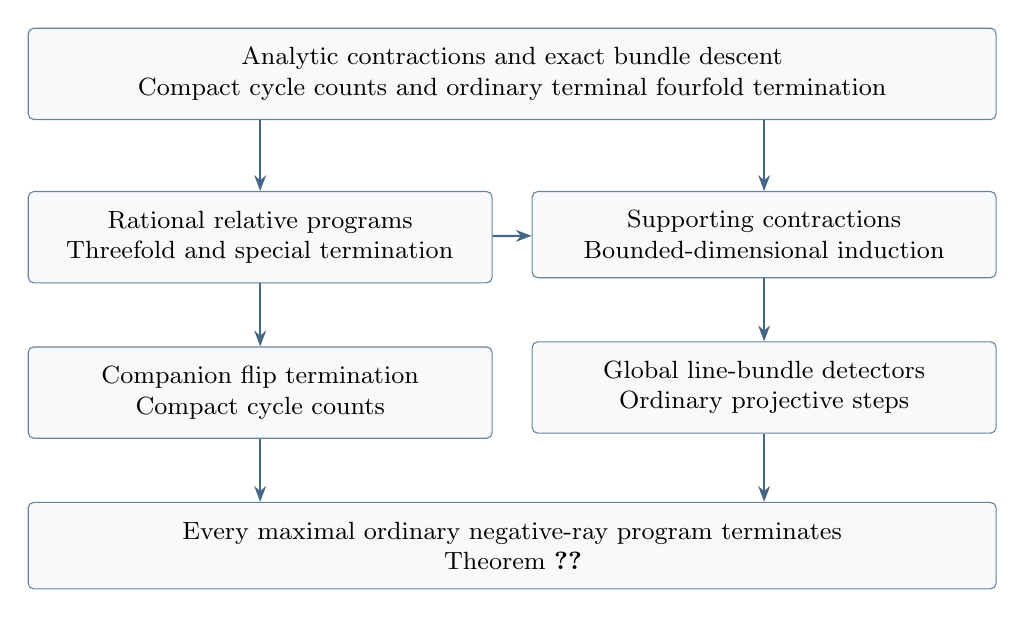
\begin{tikzpicture}[
 box/.style={draw=linkblue!65,rounded corners=2pt,align=center,
 fill=linkblue!3,text width=5.4cm,inner sep=7pt,font=\small},
 shared/.style={box,text width=11.8cm},
 edge/.style={-{Stealth[length=2mm]},draw=linkblue!80,thick}]
\node[shared] (common) {Analytic contractions and exact bundle descent\\
Compact cycle counts and ordinary terminal fourfold termination};
\node[box,below=9mm of common.south west,anchor=north west] (relative)
 {Rational relative programs\\
Threefold and special termination};
\node[box,below=9mm of common.south east,anchor=north east] (supporting)
 {Supporting contractions\\
Bounded-dimensional induction};
\node[box,below=8mm of relative] (companion)
 {Companion flip termination\\
Compact cycle counts};
\node[box,below=8mm of supporting] (ordinary)
 {Global line-bundle detectors\\
Ordinary projective steps};
\node[shared,below=8mm of companion.south west,anchor=north west] (finite)
 {Every maximal ordinary negative-ray program terminates\\
Theorem~\ref{thm:finite}};
\draw[edge] (common.south -| relative.north)--(relative.north);
\draw[edge] (common.south -| supporting.north)--(supporting.north);
\draw[edge] (relative)--(supporting);
\draw[edge] (relative)--(companion);
\draw[edge] (supporting)--(ordinary);
\draw[edge] (companion.south)--(finite.north -| companion.south);
\draw[edge] (ordinary.south)--(finite.north -| ordinary.south);
\end{tikzpicture}
\caption{Dependencies in the proof of Theorem~\ref{thm:finite}. The
relative and lower-dimensional results support the contraction induction
and the companion flip-termination theorem.}
\label{fig:dependencies}
\end{figure}


\section{Classes, currents, and exceptional divisors}\label{sec:analytic}

The scaling argument transports one K\"ahler form from the original
space through several birational models.  Its trace need not be smooth,
or even have local potentials without further argument.  We establish
the precise trace relation, its positivity, and the comparison rules
used below.  Equalities between Bott--Chern classes will be distinguished
from equalities between divisors or currents.

\subsection{Pullback of classes}

We use the following cohomological descent theorem.  A space is in
\emph{Fujiki's class $\mathcal C$} if it is bimeromorphic to a compact
K\"ahler manifold.

\begin{lemma}[Pullback and descent]\label{lem:pullback-image}
Let $f:T\to Z$ be a proper surjective morphism with connected fibres between normal
compact analytic spaces with rational singularities.  Suppose that $T$
is in class $\mathcal C$ and that either the general fibre is rationally
connected or $R^jf_*\cO_T=0$ for every $j>0$.  Then
\[
 f^*: \BC(Z)\longrightarrow\BC(T)
\]
is injective, and its image consists exactly of the classes having
degree zero on every $f$-vertical curve.  If $T$ and $Z$ are K\"ahler,
a class on $Z$ is nef if and only if its pullback is nef.
\end{lemma}

\begin{proof}
The pullback assertion is \cite[Lemma~2.39]{HX2026}; nef descent is
\cite[Lemma~2.38]{DHP2024}.  In particular, the first assertion applies
to any proper bimeromorphic morphism between compact spaces with
rational singularities whose source is in class $\mathcal C$: its
general fibre is a point.  For a projective klt log Fano contraction,
relative vanishing supplies the higher-direct-image hypothesis once
rationality of the base has been established.
\end{proof}

\subsection{Positive currents on a normal model}

An $f$-exceptional real divisor is a finite real linear combination of
prime divisors whose images have codimension at least two.
We next give the descent statement needed when an exceptional
correction has either sign.  Pseudo-effectivity requires a positive
current with local plurisubharmonic potentials; we do not assume
that an arbitrary positive current on a singular space has them.

\begin{lemma}[Exceptional descent]\label{lem:positive-descent}
Let $p:U\to T$ be a resolution of a normal compact K\"ahler space,
with $U$ compact K\"ahler.  Let $\alpha\in\BC(T)$ and let $E$ be a
$p$-exceptional real divisor.  If $p^*\alpha+[E]$ is pseudo-effective,
then $\alpha$ is pseudo-effective.  No sign condition on $E$ is needed.
Pseudo-effective classes pull back to resolutions, and nef classes
on $T$ are pseudo-effective.
\end{lemma}

\begin{proof}
Choose a smooth representative $\theta$ of $\alpha$ with local smooth
potentials.  On the smooth compact K\"ahler space $U$, a positive
representative of the given class has the form
\begin{equation}\label{eq:positive-upstairs}
 S=p^*\theta+[E]+\ddc v
\end{equation}
for a global distribution $v$.  Remove from $T$ its singular locus
and the image of the exceptional locus, obtaining a smooth open set
$T^\circ$ whose complement has codimension at least two.  The map
$p$ is an isomorphism there.  Equation~\eqref{eq:positive-upstairs}
gives a global $\theta$-plurisubharmonic function $v^\circ$ on
$T^\circ$.  We do not assert that $v$ is quasi-plurisubharmonic along
$E$.

On a coordinate neighbourhood where $\theta=\ddc\rho$, extend
$\rho+v^\circ$ first across the removed codimension-two subset of
the regular locus, and then across the singular locus.  The first
extension is the plurisubharmonic Hartogs theorem; the second is its
normal-space version of Grauert--Remmert, recalled in
\cite[Section~2.1, pp.~927--928]{CMM2017}.  These extensions are unique.
On overlaps their differences are the original smooth
pluriharmonic differences of the functions $\rho$.  Subtracting
$\rho$ therefore gives a global potential $v_T$, and
\[
 \theta+\ddc v_T\geq0
\]
is a current with local plurisubharmonic potentials representing
exactly $\alpha$.  This proves descent, including for signed $E$.

For pullback, compose local plurisubharmonic potentials with the
resolution.  They cannot become identically $-\infty$ on a nonempty
open subset, since a resolution is an isomorphism on a dense open
set.  Thus they define the pulled-back positive current; see
\cite[Section~2.1, p.~928]{CMM2017}.

Finally, if $\alpha$ is nef, then $p^*\alpha$ is nef on $U$.
For a K\"ahler form $\omega_U$, choose positive representatives of
$p^*\alpha+\varepsilon[\omega_U]$.  Their masses are bounded as
$\varepsilon\downarrow0$, so a weak limit is a positive current in
$p^*\alpha$.  On the smooth K\"ahler manifold $U$ it has local
plurisubharmonic potentials.  The first part, with $E=0$, descends
this current to the required class on $T$.
\end{proof}

\subsection{Generalized pairs and negativity}

We recall the generalized-pair language in the form needed here
\cite[Section~2.1 and Definition~2.7]{DHY2023}.  A closed \emph{b-$(1,1)$
current} is a compatible collection of closed $(1,1)$-currents on
proper birational models: pushforward along a morphism between models
recovers the current on the lower model.  It \emph{descends} to a
model $U$ if its trace there and all higher traces have local
potentials, and the classes of the higher traces are pullbacks of
its class on $U$.
It is \emph{b-nef} if that class is nef on some such model.
We also use the relative version for real combinations of line-bundle
data on a carrier projective over a specified base.  Here nefness
means nonnegative degree on curves contracted to that base.  The
structure equation and discrepancy definition below are unchanged.

A generalized pair on $T$ consists of a boundary $B\geq0$, a b-nef
datum $\mathbf M$, and a log resolution $\nu:U\to T$ on which the
datum descends, together with an actual real divisor $B_U$ such that
$\nu_*B_U=B$ and
\begin{equation}\label{eq:generalized-structure}
 [K_U+B_U]+[\mathbf M_U]=\nu^*L,
 \qquad L\in\BC(T).
\end{equation}
The support of $B_U$ may be taken to have simple normal crossings.
Negativity makes this structure boundary unique; passing to higher
resolutions gives the other structure boundaries.  The generalized
log discrepancy of a prime $P$ on such a resolution is
\[
 a(P,T,B+\mathbf M)=1-\operatorname{coeff}_P B_U.
\]
The pair is generalized klt, or \emph{gklt}, if all these discrepancies
are positive, and generalized log canonical, or \emph{glc}, if they
are all nonnegative.  The \emph{gklt locus} is the open subset where
all discrepancies of primes centred there are positive; its
complement is the generalized non-klt locus.  We use the word
\emph{terminal} for an ordinary or
generalized klt pair whose discrepancies at all exceptional primes
are strictly greater than one.  Negative coefficients are permitted
in $B_U$, although the boundary $B$ on the model is effective.
Generalized klt spaces have rational singularities
\cite[Theorem~2.19]{DHY2023}.

The negativity lemma concerns actual divisors, not arbitrary
Bott--Chern classes.  We record also the strict form needed for
fourfold termination.

\begin{lemma}[Negativity and strict comparison]\label{lem:negativity}
\leavevmode
\begin{enumerate}[label=\textup{(\roman*)}]
\item Let $f:T\to Z$ be a proper bimeromorphic morphism of normal
complex spaces and let $E$ be a real Cartier divisor such that $-E$
is $f$-nef.  Then $E\geq0$ if and only if $f_*E\geq0$.
Consequently an $f$-exceptional, $f$-numerically trivial real Cartier
divisor is zero.
\item If, in addition, $f$ has connected projective fibres and
$E\geq0$ is $f$-anti-nef, then every fibre is either contained in
$\Supp E$ or disjoint from $\Supp E$.
\item Consider a nontrivial small birational diagram
\[
 T\xrightarrow{\ f\ }Z\xleftarrow{\ f^+\ }T^+
\]
of normal compact spaces, with projective contractions on both
sides.  Let $B\geq0$ be a real boundary, let $B^+$ be its strict
transform, and suppose the ordinary adjoints
$D=K_T+B$ and $D^+=K_{T^+}+B^+$ are real Cartier, with $-D$ relatively
ample on the left and $D^+$ relatively ample on the right.
The two exceptional loci have the same image $A\subset Z$.  On a
common resolution $p:V\to T$, $q:V\to T^+$,
\begin{equation}\label{eq:ordinary-flip-comparison}
 p^*D-q^*D^+=F,\qquad F\geq0,
\end{equation}
where $F$ is an actual divisor exceptional over both models.
For every prime divisor $P$ over these spaces,
\[
 a(P,T^+,B^+)\geq a(P,T,B),
\]
and the inequality is strict if the centre of $P$ on either side
is contained in that side's exceptional locus.
\item For the diagram in \textup{(iii)}, if $\dim T=4$, then $\dim A\leq1$ and
\[
 \dim\Exc(f)+\dim\Exc(f^+)\geq3.
\]
\item The discrepancy conclusions in \textup{(iii)} also hold for
generalized pairs with the same fixed b-nef datum and transformed
boundaries in a projective small diagram, provided the source log
class has negative degree on every curve contracted on that side,
and the target log class has positive degree on every curve
contracted on the other side.  They hold likewise for a projective divisorial
contraction $f:T\to T'$ when the target boundary is the pushforward,
the b-datum is unchanged, and the source log class has negative
degree on every $f$-vertical curve.  In this divisorial case strictness holds at every prime
whose source centre lies in $\Exc(f)$.
This part also applies when the fixed b-datum is nef only over a
specified base.
\end{enumerate}
\end{lemma}

\begin{proof}
Part~(i) is the analytic negativity lemma
\cite[Lemma~2.5]{HX2026}; apply it to both signs for the last assertion.
For (ii), points of a connected projective fibre can be joined by a
chain of irreducible curves.  If the fibre met both $\Supp E$ and
its complement, some curve in such a chain would meet the support
without being contained in it.  Its intersection with the effective
real Cartier divisor would be strictly positive, contrary to
$f$-anti-nefness.  The assertion for a real Cartier divisor follows
locally from positive combinations of effective rational Cartier
divisors, as explained below.

For (iii), let $G$ be the normalization of the graph in
$T\times_ZT^+$, with projections $p_G,q_G$ and map $h:G\to Z$.
Compatible canonical data give the actual real Cartier divisor
\[
 F_G=p_G^*D-q_G^*D^+.
\]
This difference is defined locally by compatible meromorphic canonical
generators and therefore glues, even when the canonical sheaves were
specified as $\Q$-line bundles.  Smallness makes it exceptional over
both sides.  It is effective by (i), applied over $T$: on a
$p_G$-vertical curve the degree of $-F_G$ is the degree of
$q_G^*D^+$, which is nonnegative.

For every $h$-vertical curve $C$ one has
\begin{equation}\label{eq:graph-strict-degree}
 F_G\cdot C<0.
\end{equation}
Indeed, normalization is finite onto the graph, so the two projections
cannot both contract $C$.  The nonzero degrees contributed by $p_G^*D$
and $-q_G^*D^+$ are both negative.  An effective real Cartier divisor
has nonnegative degree on a curve outside its support.  For completeness,
this fact and its strict pullback analogue hold even if its individual
prime components are not $\Q$-Cartier: locally express it in the real
span of finitely many Cartier divisors.  Vanishing of coefficients
outside its support and nonnegativity of the remaining coefficients
are rational linear conditions.  The resulting rational polyhedral
cone expresses it as a positive real combination of effective
$\Q$-Cartier divisors.  The usual effective Cartier assertions apply
to each term; summing the nonnegative local intersection numbers
gives the asserted global degree inequality.  In particular, the pullback has positive coefficient
at every prime whose centre is contained in the support.

The morphism $p_G$ has connected fibres because $T$ is normal;
hence $h=f p_G$ has connected fibres.  Its fibres are projective
because $G$ is finite over the graph in the fibre product.  Each
point of a positive-dimensional fibre lies on a curve in that fibre.  Equation
\eqref{eq:graph-strict-degree} therefore places the entire fibre in
$\Supp F_G$.  To identify the relevant fibres, suppose $f$ is an
isomorphism over an open subset of $Z$.  There the log divisor on
$T^+$ is pulled back from $Z$, by smallness and agreement in codimension
one.  Relative ampleness excludes an $f^+$-vertical curve there;
projectivity, connectedness and normality then make $f^+$ an
isomorphism there as well.  Interchanging the sides proves that their
exceptional images coincide.  Thus $h^{-1}(A)\subset\Supp F_G$.

Pull $F_G$ back to a resolution on which $P$ appears.  Its coefficient
at $P$ is exactly
$a(P,T^+,B^+)-a(P,T,B)$, with our log-discrepancy convention.
Effectivity gives monotonicity, and the support assertion gives the
claimed strictness.  This proves (iii).

For (iv), a small exceptional locus in a fourfold has dimension at
most two and has positive-dimensional fibres, so its image has
dimension at most one.  Moreover $F_G\ne0$ by
\eqref{eq:graph-strict-degree}.  A component of its support has
dimension three and maps finitely into
$\Exc(f)\times_Z\Exc(f^+)$.  The dimension of this product is at most
the sum of the dimensions of its two factors.  This proves (iv).

For (v), choose a common smooth resolution $p:V\to T$,
$q:V\to T'$ carrying the fixed b-datum and projective over the
common contraction base.  Such a resolution is obtained by taking
projective modifications of the graph that resolve the maps to a
carrier of the datum.  Subtract the actual
structure boundaries to obtain a real Cartier divisor
$F=B_{T,V}-B_{T',V}$.  Its coefficients are the differences of
generalized log discrepancies, and cancellation of the fixed
b-part gives
\[
 [F]=p^*L_T-q^*L_{T'}.
\]
Let $h:V\to Z$ be the morphism to the common contraction base;
in the divisorial case $Z=T'$ and $q=h$.  It is projective by this
choice and has connected fibres because it is bimeromorphic onto
the normal space $Z$.  The boundary-pushforward
condition makes $F$ exceptional over $Z$.  The relative signs of
the log classes give $F\cdot C\leq0$ on every $h$-vertical curve,
with strict inequality whenever $p(C)$ or, in the small case,
$q(C)$ is a curve.  Thus (i) gives $F\geq0$.

If $y$ lies in an exceptional image, a vertical curve downstairs
can be lifted to a curve on $V$ dominating it: use a component of
its projective inverse image and cut by relatively ample
hyperplanes.  Such a curve has negative $F$-degree and hence lies
in $\Supp F$.  Part~(ii) now puts the entire fibre $h^{-1}(y)$ in
the support.  Pullback to a higher resolution has positive
coefficient at every prime centred in this support.  This proves
all the strict discrepancy inequalities, including for a centre
on the flipped side.  No trace current on the normalized graph
is assumed to be Cartier; the actual divisor is constructed from
the structure boundaries on the smooth resolution.
\end{proof}

\subsection{A fixed nef b-part and its traces}

For the finite-program proof, fix a K\"ahler form $h$ on the original
space $X$, and set $H=[h]$.  It defines a positive b-current
$\mathbf H$: for a marked birational model $T$, choose a common
resolution $p:V\to T$, $q:V\to X$ and put
\begin{equation}\label{eq:actual-H-trace}
 \mathbf H_T=p_*q^*h.
\end{equation}
Compatibility on higher resolutions makes this independent of the
choice of resolution \cite[Claim~2.5]{DHY2023}.  Throughout the proof
this is one fixed current datum; we do not replace it by arbitrary
cohomologous currents.  The class of the trace, when it exists, will
be denoted by $H_T$.

\begin{lemma}[The exceptional trace relation]\label{lem:class-trace}
Let $T$ be a normal compact K\"ahler space with rational singularities,
marked birationally to $X$.  Suppose that on a common smooth K\"ahler
resolution $p:V\to T$, $q:V\to X$ there are a class $H_T\in\BC(T)$
and an actual $p$-exceptional real divisor $J_T$ satisfying
\begin{equation}\label{eq:class-trace}
 p^*H_T=q^*H+[J_T].
\end{equation}
Then $J_T\geq0$.  The class $H_T$ and the divisor $J_T$ are unique,
and the correction on a higher resolution is the pullback of $J_T$.

For an effective boundary $B_T$ with real Cartier ordinary adjoint,
the generalized structure boundary for the nef datum $t\mathbf H$ is
\begin{equation}\label{eq:trace-boundary}
 B_{T,V}(t)=p^*(K_T+B_T)-K_V+tJ_T,\qquad t\geq0.
\end{equation}
In particular, decreasing $t$ increases every generalized log
discrepancy.  If the generalized pair is gklt, its ordinary pair is
klt; if all its exceptional log discrepancies exceed one, the
ordinary pair is terminal.

Conversely, suppose $t>0$ and a generalized pair with boundary $B_T$
and this fixed datum $t\mathbf H$ is given by
\eqref{eq:generalized-structure}, with log class $L$ and real Cartier
ordinary adjoint.  Then \eqref{eq:class-trace} holds with
\[
 H_T=\frac{L-[K_T+B_T]}{t}.
\]
\end{lemma}

\begin{proof}
On every $p$-vertical curve, $-J_T$ has the same degree as the nef
class $q^*H$.  Lemma~\ref{lem:negativity}(i) gives $J_T\geq0$.
Subtract two possible relations.  The difference of the correction
divisors is $p$-exceptional and numerically trivial over $T$, hence
zero.  Pullback injectivity from Lemma~\ref{lem:pullback-image} then
gives uniqueness of the class as well.

Pulling back \eqref{eq:class-trace} to a higher resolution gives the
claimed correction there by uniqueness.  Conversely, if the relation
is initially known on a higher resolution $r:V'\to V$, push its
correction down to $V$.  The difference between the upstairs
correction and the pullback of this pushforward is $r$-exceptional
and numerically trivial over $V$, so is zero.  Injectivity of $r^*$
gives the relation on $V$.

Equation~\eqref{eq:trace-boundary} follows by adding $K_V$ and the
fixed nef class $tq^*H$ to its two sides.  Its coefficients give
\[
 a(P,T,B_T+t\mathbf H)
 =a(P,T,B_T)-t\operatorname{coeff}_P J_T
\]
on every sufficiently high resolution.  This proves the discrepancy
assertions.

For the converse, let $B_V$ be the given actual generalized structure
boundary and put $B_V^{\rm ord}=p^*(K_T+B_T)-K_V$.  Both push forward
to $B_T$, so
\[
 J_T=\frac{B_V-B_V^{\rm ord}}{t}
\]
is an actual $p$-exceptional divisor.  Subtract the ordinary log class
from \eqref{eq:generalized-structure} to obtain
\eqref{eq:class-trace}.  This constructs the divisor before applying
negativity; it does not infer a divisor from an arbitrary class
difference.
\end{proof}

The converse is particularly useful for an extraction carrying a
pulled-back generalized log class.  It shows that the divided
difference defining its trace is the same class whenever the marked
model is the same, even if its boundary was obtained at a different
scaling parameter.

\begin{corollary}[Positivity of the trace]\label{cor:big-trace}
Under the hypotheses of Lemma~\ref{lem:class-trace}, the actual trace
$\mathbf H_T$ has local plurisubharmonic potentials and represents
$H_T$.  The class $H_T$ is big.
\end{corollary}

\begin{proof}
The positive current $q^*h+[J_T]$ represents $p^*H_T$.
The proof of Lemma~\ref{lem:positive-descent} constructs a positive
current $S_T$ in $H_T$ with local potentials.  On the big open where
$p$ is an isomorphism and the correction is absent, it agrees with
$p_*q^*h$.  Their difference is a closed current of order zero
supported in codimension at least two.  Such a current vanishes:
after a local embedding it has bidimension
$(\dim T-1,\dim T-1)$, whereas its support has smaller dimension
\cite[Chapter~III, Corollary~2.11]{DemaillyCADG2012}.
Thus $S_T$ is precisely the actual trace in
\eqref{eq:actual-H-trace}.  This step is needed because a trace of
a positive b-current need not have local potentials a priori
\cite[Remark~2.6(ii)]{DHY2023}.

The class $q^*H$ is nef and has positive top self-intersection:
$q^*h$ is semipositive and is positive on the dense open where $q$
is an isomorphism.  By \cite[Theorem~0.5]{DemaillyPaun2004}, it contains
a K\"ahler current $R\geq\delta\omega_V$ for some $\delta>0$ and
some K\"ahler form $\omega_V$.  Fix a K\"ahler form $\omega_T$ and
choose $C>0$ with $p^*\omega_T\leq C\omega_V$.  For
$0<\varepsilon<\delta/C$,
\[
 R+[J_T]-\varepsilon p^*\omega_T\geq0.
\]
Its class is $p^*(H_T-\varepsilon[\omega_T])$.
Lemma~\ref{lem:positive-descent} shows that
$H_T-\varepsilon[\omega_T]$ is pseudo-effective.  Hence $H_T$
contains a K\"ahler current, as required.
\end{proof}

\subsection{Comparison with the same nef datum}

The preceding results supply the positivity needed for scaling.  We
finish with the comparison that later excludes divisorial steps in
the limiting program and identifies the two nef pullbacks in the
final contradiction.

\begin{lemma}[Small-model comparison]\label{lem:small-comparison}
Let $(T,B_T+\mathbf M)$ and $(T',B_{T'}+\mathbf M)$ be generalized
pairs with the same b-nef datum, whose log classes are $L_T$ and
$L_{T'}$.  Suppose the marked birational map $T\dashrightarrow T'$
extracts no divisors and $B_{T'}$ is the pushforward of $B_T$.
On a common sufficiently high resolution $p:V\to T$, $q:V\to T'$, put
\[
 F=B_{T,V}-B_{T',V}.
\]
Then $F$ is an actual divisor exceptional over $T'$, and
\begin{equation}\label{eq:small-comparison}
 p^*L_T-q^*L_{T'}=[F],\qquad
 \operatorname{coeff}_P F
 =a(P,T',B_{T'}+\mathbf M)-a(P,T,B_T+\mathbf M).
\end{equation}
If the map is small, $F$ is exceptional over both models.  In this
case nefness of $L_{T'}$ implies $F\geq0$, and nefness of both log
classes implies $F=0$.  These conclusions also hold relatively over
a common base.  In particular equal pullback classes imply equality
of the structure boundaries.
\end{lemma}

\begin{proof}
Subtract the two structure equations on $V$.  The trace of the fixed
b-datum cancels, giving \eqref{eq:small-comparison}.  At a prime
dominating a divisor on $T'$, the corresponding boundary coefficient
on $T$ is unchanged, so its coefficient in $F$ is zero.  This proves
exceptionality over $T'$.  Smallness gives the same assertion over
$T$.

If $L_{T'}$ is nef, then $-F$ is $p$-nef, because its degree on a
$p$-vertical curve is the degree of $q^*L_{T'}$.  Negativity gives
$F\geq0$.  If $L_T$ is also nef, then $F$ is $q$-nef, so applying
negativity with the opposite sign gives $F\leq0$.  The same proof
uses only relative nefness when the models lie over a common base.
For equal pullback classes, the already constructed exceptional
divisor is relatively numerically trivial, and is zero by
Lemma~\ref{lem:negativity}(i).
\end{proof}

All equalities of pulled-back log classes in this lemma are
cohomological.  Equality of actual currents was used only in the
separate trace-identification argument.  These distinctions allow
the ordinary steps and the generalized auxiliary constructions to
share one fixed nef datum.

\section{Ordinary steps on the given space}\label{sec:absolute}

We construct the contraction and flip of every negative analytic ray in
arbitrary dimension.  The input is an ordinary rational klt pair in the
\emph{global Weil-divisor} category.  Generalized pairs enter only through
the cone and base-point-free theorems; the steps themselves are ordinary.
The main point is to preserve actual line bundles, including their fixed
Cartier indices, rather than only numerical classes.

\subsection{Integral descent}

Bundles are written additively in numerical expressions.  For example,
$L-(K_T+C)$ denotes the rational line bundle obtained from $L$ and the
rational adjoint.  All degrees in the following lemma are degrees on
compact curves contracted by the indicated morphism.

\begin{lemma}[Integral descent]\label{lem:descent}
Let $f:T\to Z$ be a projective bimeromorphic contraction of normal complex
spaces, and let $L$ be a line bundle numerically trivial over $Z$.
Suppose that every point of $Z$ has a neighbourhood $U$ on which there is
an ordinary rational klt pair $(f^{-1}U,C_U)$ with rational adjoint and
\[
 L-(K_{f^{-1}U}+C_U)\quad\text{$f$-nef over $U$}.
\]
Then $f_*L$ is a line bundle and the evaluation map is an isomorphism
\begin{equation}\label{eq:integral-descent}
 f^*f_*L\simeq L.
\end{equation}
In particular the conclusion applies if the local ordinary adjoints are
relatively antiample.  It also applies to a global ordinary rational klt
pair $(T,C)$ whenever $L-(K_T+C)$ is $f$-nef.  Clearing one denominator
therefore descends a rational line bundle as an actual rational line
bundle.
\end{lemma}

\begin{proof}
Fix $z\in Z$ and shrink to a connected Stein neighbourhood $U$ on which
the stated pair is defined.  A line bundle $M$ on $f^{-1}U$ has a
Cartier-divisor representative there: the coherent direct image $f_*M$
has rank one over the nonempty open where $f$ is an isomorphism, so
Cartan's Theorem~A supplies a nonzero section.  Its pullback is a section
of $M$ that is not identically zero, and its zero divisor is Cartier.
This argument takes place over $U$, not on the whole compact space.

Every rational line bundle $N$ on $f^{-1}U$ is also relatively big.
Indeed, choose $q>0$ with $qN$ a line bundle and an $f$-ample line bundle
$A$.  The same direct-image argument gives a nonzero section of
$qN-A$, hence
\[
 N\simq q^{-1}A+q^{-1}E\qquad(E\geq0).
\]
This is relative bigness in the analytic sense
\cite[Definition~2.46]{Fujino2022}.  Apply it to
$N=L-(K_T+C_U)$.  The klt base-point-free theorem gives, after shrinking
around $z$, relative generation of $L^k$ for \emph{every} sufficiently
large integer $k$ \cite[Theorem~6.2 and Remark~6.3]{Fujino2022}.

Choose finitely many such generating sections near the compact fibre
$F=f^{-1}(z)$.  The morphism they define on the projective reduced fibre
$F_{\mathrm{red}}$ is constant on each irreducible component: a
positive-dimensional image would yield a curve with positive degree
against the pullback of the hyperplane bundle, contrary to the
numerical triviality of $L^k$.  Such a curve is obtained by successive
general hyperplane sections of a component.  Connectedness of $F$ makes
the images of all its components the same point.  A linear combination
of the generating sections is consequently nonzero at every point of
$F_{\mathrm{red}}$.

This section is a generator of $L^k$ in the local ring at every point of
$F$: its residue is nonzero, and hence its representing function is a
unit.  This also treats a nonreduced fibre.  Properness allows us to
shrink $U$ away from the image of the section's zero set.  Thus $L^k$ is
trivial on $f^{-1}U$.  Apply the argument to consecutive integers $k$ and
$k+1$, and use one common neighbourhood.  Their quotient trivializes
$L$ itself.  Since $f_*\cO_T=\cO_Z$, on this neighbourhood $f_*L\simeq
\cO_U$, and evaluation is an isomorphism.  These local conclusions give
\eqref{eq:integral-descent} globally.  No additional tensor power enters
the integral conclusion.
\end{proof}

The nef variant is important even when the adjoint has degree zero over
$f$.  For example, if $P=K_T+C$ is a rational klt adjoint, $\ell P$ is
Cartier, and $P$ is numerically trivial over $f$, apply
Lemma~\ref{lem:descent} to $L=\ell P$.  Its difference from the adjoint
is $(\ell-1)P$, so the \emph{same} index $\ell$ descends.

\subsection{Supporting classes and projectivity}

A class is \emph{modified big} if it is the birational pushforward of a big class
\cite[Definition~2.8]{HX2026}. In particular, a big class is modified big.

We use the generalized cone theorem
\cite[Theorem~1.3]{HX2026}. For a compact K\"ahler gklt pair with a
descending nef part $\beta$, the cone $\NA(T)$ is the sum of its
adjoint-nonnegative part and rays of rational curves. Only finitely many
rays are needed when the boundary plus $\beta$ is big. The supporting
contractions needed in dimensions at most four are proved in
Proposition~\ref{repair:prop:supporting-contraction}. Their projectivity
will be obtained from the ordinary rational adjoint.

\begin{lemma}[Supports with a K\"ahler margin]\label{lem:absolute-support}
Let $(T,B)$ be an ordinary rational klt pair on a normal compact K\"ahler
space.  Assume that $B$ is $\Q$-Cartier and that $D=K_T+B$ is a rational
line bundle.  If $D$ is not nef, $\NA(T)$ has a $D$-negative extremal ray.
Every such ray $R$ is generated by a rational curve and has a nonempty
relatively open set $\mathcal U_R\subset R^\perp$ of classes satisfying
\begin{equation}\label{eq:absolute-support}
 \alpha\text{ is nef},\qquad
 \NA(T)\cap\alpha^\perp=R,\qquad
 \alpha-c_1(D)\text{ is K\"ahler}.
\end{equation}
\end{lemma}

\begin{proof}
Fix a K\"ahler class $\omega$ and write $d=c_1(D)$.  Cone duality applies
because klt singularities are rational.  The slice
\[
 S=\{v\in\NA(T):\omega\cdot v=1\}
\]
is compact.  Indeed, fix smooth representatives of a basis of $\BC(T)$.
Each is bounded above and below by a multiple of a K\"ahler form, so all
its pairings on $S$ are bounded; the slice is closed.  If $D$ is not nef,
the minimum of $d$ on $S$ is negative.  An extreme point of its minimum
face gives a negative extremal ray.

Fix any such ray and let $r\in S$ be its normalized point.  Choose
$\varepsilon>0$ with $(d+\varepsilon\omega)\cdot r<0$.  The descending
nef part $\varepsilon\omega$ changes no discrepancy, and
$B+\varepsilon\omega$ is big since $B$ is effective and $\Q$-Cartier.
The finite form of the cone theorem gives
\begin{equation}\label{eq:absolute-finite-cone}
 \NA(T)=\NA(T)_{d+\varepsilon\omega\geq0}
       +\sum_{j=1}^{N}\R_{\geq0}[C_j],
\end{equation}
where the $C_j$ are rational curves.  Normalize their classes in $S$
and discard repetitions.  By extremality, $r$ is one of these points,
say $r_1$.  Let $K$ be the convex hull of the others and of
$S\cap\{d+\varepsilon\omega\geq0\}$.  This is compact and excludes
$r$; otherwise extremality of $r$ would fail.

If $K$ is nonempty, strict separation gives a linear functional $h$
with $h(r)=0$ and $h>0$ on $K$, after subtracting a multiple of $\omega$.
Regard it as a Bott--Chern class by duality.  For all sufficiently small
$\delta>0$, $h-\delta d$ is strictly positive on $K$ and at $r$.
Since $S=\operatorname{conv}(\{r\}\cup K)$, it is strictly positive on
$S$, hence K\"ahler.  Thus $\alpha=h/\delta$ has the required properties.
Its positive minimum on $K$ persists under small perturbations in
$R^\perp$; openness of the K\"ahler cone also preserves
$\alpha-d$.  These perturbations give $\mathcal U_R$.  If $K$ is empty,
then $S=\{r\}$ and $-d$ is K\"ahler; a small neighbourhood of $0$ in
$R^\perp$ has the required properties.  This includes the case
$R^\perp=\{0\}$.
\end{proof}

\begin{lemma}[Relative positivity]\label{lem:relative-positivity}
Let $f:T\to Z$ be a proper morphism of compact complex spaces, with $T$
and $Z$ K\"ahler.  Suppose that $L$ is a rational line bundle and
\[
 c_1(L)=\kappa-f^*\gamma,
\]
where $\kappa$ is K\"ahler on $T$ and $\gamma$ is a smooth real
Bott--Chern class on $Z$.  Then $L$ is $f$-ample and $f$ is projective.
Conversely, a normal space projective over a compact K\"ahler space is
compact K\"ahler if it has a global relatively ample line bundle.
\end{lemma}

\begin{proof}
Clear the denominator of $L$.  Its Bott--Chern identity permits a smooth
Hermitian metric whose curvature is the indicated difference of forms.
On every fibre its curvature is positive.  Positivity of a line bundle
on a compact complex space implies ampleness, and for a proper analytic
map ampleness on every fibre is equivalent to relative ampleness
\cite[Corollary~1.12 and Definition~3.1--Remark~3.2]{FujinoVanishing2026}.
This criterion does not presuppose projectivity and applies to
nonreduced fibres as well.  Existence of the relatively ample line bundle
makes $f$ projective.

For the converse, local relative embeddings give metrics on a relatively
ample bundle with positive curvature in fibre directions.  Glue their
weights by a partition of unity on the base.  The resulting metric
retains that positivity.  Add a sufficiently large multiple of a base
K\"ahler form to its curvature.  The sum is strictly positive; compactness
allows one multiple to work everywhere.
\end{proof}

\subsection{The ordinary contraction and flip}

We can now perform each step and preserve the category.  The next
proposition records both the numerical ranks of the negative contraction
and the actual canonical algebra of a flip.  The latter description will
also be used in the termination argument for arbitrary choices of negative rays.

\begin{proposition}[Ordinary negative steps]\label{prop:ordinary-step}
Let $(T,B)$ be an ordinary rational klt pair on a normal compact K\"ahler
space of dimension at most four, globally $\Q$-factorial in the Weil-divisor sense, with canonical
sheaf a rational line bundle.  Put $D=K_T+B$.  Every $D$-negative
extremal ray $R\subset\NA(T)$ has a projective contraction $f:T\to Z$
with connected fibres and normal compact K\"ahler target, such that
\begin{equation}\label{eq:ordinary-negative-bc}
 f^*\BC(Z)=R^\perp,\qquad
 \rho(T/Z)=1,\qquad -D\text{ is }f\text{-ample}.
\end{equation}
Here $\rho$ is the rank of global line-bundle degrees on contracted
curves.  The target has rational singularities and
$R^j f_*\cO_T=0$ for $j>0$.  If $\dim Z<\dim T$, this is a Mori fibre
space.  Otherwise $f$ is bimeromorphic, and precisely one of the
following occurs.
\begin{enumerate}[label=\textup{(\roman*)}]
\item The exceptional locus is one prime divisor $E$.  Put $T'=Z$,
$B'=f_*B$ and $D'=K_{T'}+B'$.  Then
\begin{equation}\label{eq:ordinary-divisorial-difference}
 D=f^*D'+eE\qquad(e>0).
\end{equation}
\item The contraction is small.  For an adjoint Cartier index $r>0$,
the intrinsic algebra
\begin{equation}\label{eq:ordinary-flip-algebra}
 \cR_r=\bigoplus_{m\geq0}f_*\cO_T(mrD)
\end{equation}
is locally finitely generated, and $T'=\Proj_Z\cR_r$ is the ordinary
flip.  It has a small projective morphism $f^+:T'\to Z$ with connected
fibres.  Put $B'=\phi_*B$ and $D'=K_{T'}+B'$, where
$\phi:T\dashrightarrow T'$ is the induced small map.  For a sufficiently
divisible choice of $r$ there is an actual isomorphism
\begin{equation}\label{eq:ordinary-tautological}
 \cO_{\Proj_Z\cR_r}(1)\simeq\cO_{T'}(rD').
\end{equation}
In particular $D'$ is a rational line bundle and is $f^+$-ample.
Passing to a sufficiently divisible Veronese leaves $T'$ unchanged.
\end{enumerate}
In both birational cases, $T'$ is compact K\"ahler and globally
Weil-divisor $\Q$-factorial, its canonical sheaf is a rational line
bundle, and $(T',B')$ is klt.  Strong global $\Q$-factoriality is
preserved when imposed on $T$.  A supplied global canonical Weil divisor
is transported to a canonical Weil divisor on $T'$.  No prime divisor is
extracted.  All log discrepancies weakly increase; the increase is strict
for every original prime contracted by the step, and, for a flip, for
every place centred in either exceptional locus.
\end{proposition}

\begin{proof}
Choose $\alpha\in\mathcal U_R$ from Lemma~\ref{lem:absolute-support}
and put $\kappa=\alpha-c_1(D)$. Proposition~\ref{repair:prop:supporting-contraction}
gives $f:T\to Z$ and $\gamma$ K\"ahler with $\alpha=f^*\gamma$.
Thus $c_1(-D)=\kappa-f^*\gamma$, and
Lemma~\ref{lem:relative-positivity} proves projectivity and relative
ampleness.  This establishes projectivity without strong factoriality.
For every curve $C\subset T$,
\begin{equation}\label{eq:ordinary-contracted-curves}
 f(C)\text{ is a point}\quad\Longleftrightarrow\quad
 \alpha\cdot C=0\quad\Longleftrightarrow\quad[C]\in R.
\end{equation}
The rational curve generating $R$ is contracted, so $f$ is nontrivial.

Relative vanishing gives $R^j f_*\cO_T=0$ for $j>0$
\cite[Theorem~5.2]{Fujino2022}; the log Fano base has rational
singularities \cite[Lemma~8.8]{DHP2024}.  Lemma~\ref{lem:pullback-image}
now identifies $f^*\BC(Z)$ with the classes of degree zero on all
vertical curves, which is exactly $R^\perp$.  The global line-bundle
rank is also one, since all those curves are proportional and the
rational line bundle $D$ detects their ray.  This proves
\eqref{eq:ordinary-negative-bc}.  The lower-dimensional case has all
the stated Mori fibre-space properties.  In equal dimension,
connectedness gives generic degree one, so $f$ is bimeromorphic.

\smallskip\noindent
\emph{Divisorial contractions.}
Suppose $E$ is an exceptional prime.  It is $\Q$-Cartier.  If
$E\cdot R\geq0$, it would be $f$-nef, contradicting negativity for a
nonzero effective exceptional divisor.  Thus $E\cdot R<0$.  Every
vertical curve lies in $E$, since an effective $\Q$-Cartier divisor
has nonnegative degree on a curve outside its support.  Every
positive-dimensional projective fibre is covered by curves.  A
zero-dimensional local component of a connected fibre would be isolated,
and the birational form of Zariski's main theorem would make $f$ an
isomorphism there.  Consequently $\Exc(f)=E$.

For a prime Weil divisor $A_Z$ on $Z$, let $A_T$ be its strict transform.
Choose $t\in\Q$ so $(A_T+tE)\cdot R=0$.  The coefficient is rational
by taking the ratio of the two rational degrees on one integral curve.
A Cartier multiple of $A_T+tE$ descends by Lemma~\ref{lem:descent}:
its difference from $D$ is relatively ample.  The descended line bundle
agrees with the corresponding reflexive power of $\cO_Z(A_Z)$ off
$f(E)$, a subset of codimension at least two.  Reflexivity identifies
them everywhere.  Hence every global prime on $Z$ is $\Q$-Cartier.

If a global canonical Weil divisor is given, push it forward.  It agrees
with the canonical sheaf on the big open where $f$ is an isomorphism, so
reflexivity shows that it remains a canonical Weil representative.
Alternatively, start with an invertible reflexive power of $\omega_T$,
adjust it by a rational multiple of $E$ to degree zero, and descend after
clearing denominators.  On the same big open the result is a reflexive
power of $\omega_Z$; hence that power is invertible everywhere.  This
proves the canonical assertion without assuming a global meromorphic
canonical section.

Now $D'$ is a rational line bundle and its canonical identification away
from $E$ gives \eqref{eq:ordinary-divisorial-difference}.  Intersection
with $R$ gives $e>0$.  If $b_E$ is the coefficient of $E$ in $B$, then
\[
 a(E;Z,B')=1-b_E+e>1-b_E=a(E;T,B)>0.
\]
Pullback of the effective divisor $eE$ gives weak increase for all other
log discrepancies.  Thus the target pair is klt.

\smallskip\noindent
\emph{The small canonical model.}
Suppose $f$ is small.  Finite generation of the ordinary relative log
canonical ring \cite[Theorem~1.18]{Fujino2022} gives local finite
generation of \eqref{eq:ordinary-flip-algebra}.  When canonical data are
written as sheaves, this application can be made over each Stein open
in $Z$: nonzero sections of rank-one proper direct images provide the
meromorphic representatives there.  Changing representatives induces
compatible graded isomorphisms of the intrinsic algebra.

The ordinary analytic flip theorem \cite[Theorem~1.14]{Fujino2022}
constructs precisely its relative canonical model.  It has no local
factoriality hypothesis.  Its proof glues the unique local log canonical
models, giving a normal small projective $f^+:T'\to Z$ globally.  The
fibres are connected because $Z$ is normal.  A finite cover of the
compact base permits one common sufficiently divisible Veronese
generated in degree one.  Replace $r$ by that multiple.  The resulting
tautological bundle is relatively ample and agrees with
$\cO_T(rD)$ on the common big open.  Its reflexive extension is
$\cO_{T'}(rD')$, proving \eqref{eq:ordinary-tautological} as an actual
bundle isomorphism.  This also proves that $D'$ is a rational line
bundle.  The relative Proj is invariant under this Veronese operation.
By Lemma~\ref{lem:relative-positivity}, $T'$ is compact K\"ahler.

For a global prime $A'$ on $T'$, transform it to $A$ on $T$ and choose
$t\in\Q$ so $(A+tD)\cdot R=0$.  Descend a Cartier multiple by
Lemma~\ref{lem:descent}.  On $T'$ its pullback agrees on the common big
open with the same multiple of $A'+tD'$.  Reflexivity extends the
identification; since $D'$ is already a rational line bundle, $A'$ is
$\Q$-Cartier.  This proves global Weil-divisor factoriality.  A given
canonical Weil divisor is transported on that common open and then
reflexively.  In the sheaf formulation, repeat the descent argument with
an invertible power of $\omega_T$ adjusted by $tD$; undoing the twist
by $tD'$ proves the rational-line-bundle property of $\omega_{T'}$.

On a common smooth resolution $p:V\to T$, $q:V\to T'$,
Lemma~\ref{lem:negativity} gives the actual discrepancy divisor
\begin{equation}\label{eq:ordinary-small-difference}
 p^*D=q^*D'+F,\qquad F\geq0,
\end{equation}
exceptional over both sides, with the asserted strictness over the
flipping and flipped loci.  This also proves klt preservation.

\smallskip\noindent
\emph{Optional strong factoriality.}
In the divisorial case, take any coherent rank-one reflexive sheaf
$\cF$ on $Z$.  Its reflexive pullback to $T$ is coherent of rank one.
Strong factoriality supplies an invertible reflexive power.  Adjust it
by a rational multiple of $E$, descend as above, and compare off $f(E)$.
A reflexive power of $\cF$ is therefore a line bundle.

In the small case start with such a sheaf $\cF'$ on $T'$.  On a common
smooth resolution put
\[
 \cM=(q^*\cF'/\text{torsion})^{**},\qquad
 \cF=(p_*\cM)^{**}.
\]
Here $\cM$ is a line bundle and $\cF$ is coherent reflexive of rank one;
both give the required transform on the common big open.  An invertible
power of $\cF$, adjusted by a rational multiple of $D$, descends.
Pull back the descended bundle and undo the twist by $D'$.  After
clearing denominators, reflexivity identifies the resulting line bundle
with a reflexive power of $\cF'$.  Thus the strong condition is
preserved.  Only sheaves defined on the whole compact spaces have been
used.

\end{proof}

\subsection{Transport of Bott--Chern classes}

For later scaling we need to transport one fixed nef datum.  The following
construction uses the rank of the negative contraction only.  It makes
no assertion that all Bott--Chern classes on a flipped space come from
the preceding space.

\begin{lemma}[Class transport]\label{lem:class-transport}
For a birational step of Proposition~\ref{prop:ordinary-step}, let
$f':T'\to Z$ mean $f^+$ in the small case and $\id_Z$ in the divisorial
case.  Every $\theta\in\BC(T)$ has a unique expression
$\theta=f^*\eta+s\,c_1(D)$, with $\eta\in\BC(Z)$ and $s\in\R$.
Define
\begin{equation}\label{eq:class-transport}
 \theta'= (f')^*\eta+s\,c_1(D').
\end{equation}
On a common resolution, $p^*\theta-q^*\theta'$ is the class of an
actual divisor exceptional over $T'$.  This rule sends the class of a
global Weil divisor to that of its transform or pushforward.  Moreover,
it propagates the fixed-nef-part trace relation of
Lemma~\ref{lem:class-trace}, with an actual effective exceptional
correction on the new model.  The same conclusions hold for the ordinary
real-boundary steps of Proposition~\ref{repair:prop:real}.
\end{lemma}

\begin{proof}
Since $D\cdot R\ne0$, subtracting a unique multiple of $c_1(D)$ makes
$\theta$ vanish on $R$.  Equation~\eqref{eq:ordinary-negative-bc} and
pullback injectivity give the unique $\eta$.  On a common resolution
over $Z$ the two pullbacks of $\eta$ agree.  Therefore
\[
 p^*\theta-q^*\theta'
       =s\,[p^*D-q^*D'].
\]
The expression in brackets is the actual exceptional discrepancy
divisor already constructed in the proof of the proposition.

If $\theta=c_1(A)$ for a global Weil divisor $A$, the difference
$p^*A-q^*A'$ is likewise exceptional over $T'$, where $A'$ is its
transform or pushforward.  Subtracting the two identities represents
$q^*(\theta'-c_1(A'))$ by a $q$-exceptional divisor.  That divisor is
numerically trivial over $q$, so negativity in both signs makes it
zero.  Pullback injectivity gives $\theta'=c_1(A')$.

Finally suppose the old trace $H_T$ of a fixed nef class on an earlier
model has, on a common high resolution, the relation
\[
 p^*H_T=p_0^*H+[J_T].
\]
If $H_T=f^*\eta+s\,c_1(D)$, the new correction is the actual divisor
\[
 J_{T'}=J_T-s(p^*D-q^*D'),\qquad
 q^*H_{T'}=p_0^*H+[J_{T'}].
\]
Every old exceptional divisor remains exceptional
over $T'$: neither kind of step extracts divisors.  The resulting
correction $J_{T'}$ is therefore an actual $q$-exceptional divisor.
Its negative is $q$-nef because $p_0^*H$ is nef.  Negativity gives
$J_{T'}\geq0$, and uniqueness and compatibility are those of
Lemma~\ref{lem:class-trace}.

For the stated real-boundary extension,
Proposition~\ref{repair:prop:real} supplies the ordinary step and its
negative-side Bott--Chern rank. The difference $p^*D-q^*D'$ is an actual
exceptional real discrepancy divisor, as shown in
Section~\ref{repair:sec:real}. The decomposition, transport formula,
and correction argument above therefore apply unchanged.
\end{proof}

\begin{remark}\label{rem:ordinary-continuation}
Proposition~\ref{prop:ordinary-step} starts on the given pair and can be
reapplied after every finite prefix of ordinary steps.  It allows every
negative ray.  Its construction is independent of any termination
claim, and makes no assertion about the positive-side quotient
$\BC(T')/(f^+)^*\BC(Z)$ or about equality of the full Bott--Chern ranks
across a flip.
\end{remark}

\section{Termination for ordinary terminal fourfold pairs}\label{sec:counts}

We prove termination of ordinary flips for compact K\"ahler fourfold
pairs with effective real boundary and log discrepancy $a(E)>1$
for every exceptional place.  Two finite counts
replace projectivity of the ambient fourfold: analytic cycle classes
control contractions, and low-discrepancy places control flipped surfaces.
The bases of successive projective contractions may vary.
We first establish these counts, including their generalized-pair form
needed for extraction later in the proof.

\subsection{Loss of analytic cycle classes}

For a compact complex analytic space $V$ and an integer $k\geq 0$, put
\[
 \begin{split}
 \mathcal C_k(V)
 &:=\operatorname{span}_{\R}\{[S]\in H_{2k}(V,\R):
                  S\subset V\text{ irreducible compact analytic},\ \dim S=k\},\\
 c_k(V)&:=\dim_{\R}\mathcal C_k(V).
 \end{split}
\]
Fundamental classes here use the complex orientation on the regular loci.
Compact analytic spaces admit finite triangulations compatible with any
specified finite collection of closed analytic subsets, with simplicial
dimension at most twice the complex dimension.  Thus $c_k(V)$ is finite.
We recall the abstract-space reduction to make the topology used here
explicit.  Teissier's compatible Whitney stratification
\cite[Chapter~III, Propositions~1.5 and~2.2.2]{Teissier1982} has finitely
many strata on a compact space.  Choose finitely many analytic charts
$z_j:U_j\hookrightarrow\C^{N_j}$ and nonnegative smooth cutoffs
$\rho_j$ compactly supported in these charts whose positivity sets
cover the space.  Extend $\rho_j$ and $\rho_j z_j$ by zero.  The map
\[
 x\longmapsto\bigl(\rho_j(x),\rho_j(x)z_j(x)\bigr)_j
\]
is a topological embedding into a Euclidean space.  Near a point where
$\rho_j>0$, its components extend smoothly to the ambient chart and the
$j$-th block has the smooth left inverse $(t,w)\mapsto w/t$.
It is therefore locally an ambient smooth embedding, which preserves
the Whitney conditions.  Mather's control data
\cite[Section~7, Proposition~7.1, and Section~8]{Mather1970} and
Goresky's triangulation theorem \cite[Section~5]{Goresky1978} now give
a compatible triangulation, smooth on each stratum.  Compactness makes
it finite, and smoothness on strata gives the dimension bound.
Borel--Moore localization below is then the relative simplicial-chain
sequence for a closed analytic subset and its complement.

If $V$ is K\"ahler and $S$ is such a subspace, then
\begin{equation}\label{eq:positive-cycle}
 \langle[\omega]^k,[S]\rangle=\int_{S_{\mathrm{reg}}}\omega^k>0
\end{equation}
for a K\"ahler form $\omega$ on $V$.  Thus $[S]\neq 0$, including when
$V$ or $S$ is singular.

\begin{lemma}[Cycle loss]\label{lem:cycle-loss}
Let $X\dashrightarrow Y$ be a bimeromorphic transformation of compact
K\"ahler spaces, represented by a proper bimeromorphic diagram.
Suppose it identifies
\[
 U=X\setminus A\simeq Y\setminus B,
\]
where $A$ and $B$ are closed analytic subspaces and $\dim B<k$.
Then there is a surjection
\[
 \mathcal C_k(X)\longrightarrow\mathcal C_k(Y).
\]
If $A$ contains an irreducible compact analytic $k$-dimensional subspace,
then $c_k(X)>c_k(Y)$.

Consequently, in a sequence of bimeromorphic transformations of
$n$-dimensional compact K\"ahler spaces which extract no prime divisors,
only finitely many transformations contract a prime divisor.  A small
transformation preserves $c_{n-1}$.
\end{lemma}

\begin{proof}
The Borel--Moore localization sequence for $B\subset Y$ contains
\[
 H_{2k}(B,\R)\longrightarrow H_{2k}(Y,\R)
 \xrightarrow{\ j_Y^*\ }H_{2k}^{\mathrm{BM}}(U,\R)
 \longrightarrow H_{2k-1}(B,\R).
\]
The outside groups vanish: the real dimension of $B$ is at most $2k-2$.
Thus $j_Y^*$ is an isomorphism.  Compose restriction from $X$ with its
inverse to obtain a linear map
\[
 H_{2k}(X,\R)\xrightarrow{\ j_X^*\ }H_{2k}^{\mathrm{BM}}(U,\R)
 \xrightarrow{\ (j_Y^*)^{-1}\ }H_{2k}(Y,\R).
\]
For an irreducible $k$-cycle $S\subset X$ not contained in $A$, its
restriction is the fundamental class of $S\cap U$.  Closing its image in
$Y$ gives its strict transform: analyticity follows by taking the proper
image of the corresponding strict transform in the given diagram.
The displayed map therefore sends $[S]$ to this transformed cycle class.
It sends $[S]$ to zero when $S\subset A$.

Conversely, no $k$-dimensional subspace of $Y$ is contained in $B$.
Its strict transform in $X$ consequently maps to its fundamental class.
This proves the asserted surjection of cycle spans.  If $S\subset A$
has dimension $k$, its nonzero class, by \eqref{eq:positive-cycle}, is
in the kernel.  This proves the strict inequality.

For a transformation extracting no prime divisor, choose the common
isomorphic open so that the complement in the target has codimension
at least two.  Every contracted source prime lies in the source
complement.  Apply the result with $k=n-1$ at every step.  The
nonnegative integer $c_{n-1}$ cannot decrease infinitely often.  For a
small transformation both complements have codimension at least two,
so applying the result in both directions gives equality.
\end{proof}

This argument does not assert surjectivity on full homology, and does
not compare the Bott--Chern spaces of the two models.

\subsection{Low places on compact log smooth data}

We use generalized discrepancies in the sense of
Section~\ref{sec:analytic}.  A place is called exceptional over $X$ when
its center on $X$ has codimension at least two.

\begin{lemma}[Low places and their projective realization]\label{lem:low-places}
Let $(X,B+\bM)$ be a generalized pair on a compact normal complex
space, with effective real boundary of finite support and nef
b-$(1,1)$ data descending to a model projective over $X$.  Fix a projective log resolution $p:W\to X$ carrying those data.
\begin{enumerate}[label=\textup{(\roman*)}]
\item If the pair is generalized klt, there is $\epsilon>0$ such that
every prime divisor over $X$ has log discrepancy at least $\epsilon$,
and only finitely many exceptional places have
\[
 a(E;X,B+\bM)<1+\epsilon.
\]
\item If the pair is generalized terminal and
$b=\max(\{0\}\cup\{\operatorname{coeff}_D B\})$, there are only
finitely many exceptional places with
\[
 a(E;X,B+\bM)<2-b.
\]
\item If the pair is generalized lc and $U\subset X$ is its generalized
klt locus, there is $\epsilon>0$ for which the assertion in \textup{(i)}
holds for places whose centers meet $U$.
\end{enumerate}
In each assertion the finite set of exceptional places can be represented
simultaneously by prime divisors on a smooth model projective over $X$.
In particular, any prescribed finite set of exceptional places with
$a(E;X,B+\bM)\leq 1$ for a generalized klt pair has such a realization.
This conclusion does not use an extraction or termination theorem.
\end{lemma}

\begin{proof}
Let $L\in\BC(X)$ be the generalized log class and let
$M_W=[\bM_W]$ be the nef trace class on $W$.  Write the crepant formula as
\begin{equation}\label{eq:carrier-boundary-count}
 [K_W+\Delta]+M_W=p^*L.
\end{equation}
This is the crepant boundary identity defining generalized
discrepancies; it is an equality of Bott--Chern classes when the nef
data are transcendental.  The boundary $\Delta$ is an actual real
divisor with simple normal crossing support.  Since the nef data
descend to $W$, every further generalized discrepancy is the ordinary
discrepancy for $(W,\Delta)$.  The coefficients of $\Delta$ need not be
nonnegative.  We may enlarge its listed simple normal crossing divisor
by components of coefficient zero.
Here a closed stratum means an irreducible component of an intersection
of listed components; it is smooth, and is the closure of its open
stratum.

We give the local estimate and the realization argument explicitly;
they are the log smooth calculations underlying
\cite[Proposition~2.36]{KM1998} and
\cite[Proposition~2.8]{CT2023}.
Write $\Delta=\sum_j d_jD_j$ and put $w_j=1-d_j$.
Suppose first that every $w_j$ is positive, and set
\[
 \delta=\min\bigl(\{1\}\cup\{w_j\}_j\bigr)>0.
\]
Let $E$ be exceptional over a smooth model with this log smooth
boundary.  At a general point of its center $C$, let $c=\codim C$,
and choose local parameters $x_1,\ldots,x_c$ for $C$ so that the
boundary components containing $C$ are $x_1=0,\ldots,x_r=0$.
For $v=\operatorname{ord}_E$, the Jacobian calculation gives
\begin{equation}\label{eq:coordinate-discrepancy-count}
 a(E;W,\Delta)\geq
 \sum_{j=1}^{r}(1-d_j)v(x_j)+\sum_{j=r+1}^{c}v(x_j).
\end{equation}
Indeed, on a smooth model containing $E$, with local parameter $t$
for $E$, write $x_j=t^{v(x_j)}u_j$ at its general point.  In a top
exterior differential at most one factor can use the term involving
$dt$ that lowers the order by one.  Thus the relative Jacobian has
order at least $\sum_{j=1}^c v(x_j)-1$.  Adding one and subtracting
the boundary orders proves \eqref{eq:coordinate-discrepancy-count}.
The remaining coordinates along $C$ are holomorphic and contribute
no negative orders.

In particular every discrepancy is at least $\delta$: for a divisor
already on the smooth model it is its listed weight, or one if it is
not listed; for an exceptional divisor use
\eqref{eq:coordinate-discrepancy-count}.  If $C$ is not a stratum of
the listed simple normal crossing divisor, then $c>r$.  When $r>0$,
the right hand side is at least $\delta+1$; when $r=0$, it is at
least $c\geq 2\geq\delta+1$.  Hence
\begin{equation}\label{eq:nonstratum-cutoff}
 C\text{ not a stratum}\quad\Longrightarrow\quad
 a(E;W,\Delta)\geq 1+\delta.
\end{equation}

Now fix a place $E$ with discrepancy strictly below $1+\delta$.
If it is not already a divisor on $W$, its center is a stratum by
\eqref{eq:nonstratum-cutoff}.  Blow up that closed stratum.
The center is smooth, the blowup is projective, and the new listed
boundary is again simple normal crossing.  If the center is the
intersection of the components indexed by $J$, then the new exceptional
component has weight
\begin{equation}\label{eq:stratum-weight-sum}
 w_{\mathrm{new}}=\sum_{j\in J}w_j.
\end{equation}
Thus all weights remain at least $\delta$, so the same argument
applies on the next model.  It excludes a non-stratum center at
every stage until $E$ becomes a divisor.

This process is finite.  While $E$ is exceptional, a blowup of its
smooth center of codimension $c\geq2$ changes its ordinary
empty-boundary discrepancy by
\[
 a(E;W_{\mathrm{new}},0)
 =a(E;W_{\mathrm{old}},0)-(c-1)v(\mathcal I_C).
\]
The subtracted quantity is a positive integer, whereas an ordinary
log discrepancy over a smooth space is a positive integer.
Consequently only finitely many such blowups are possible.
Thus $E$ is obtained by successive stratum blowups, which is the
meaning of a \emph{toroidal place} here.  This also realizes it on a projective model without first assuming
that the original model on which $E$ was given was projective over $X$.

For completeness, there are only finitely many such toroidal places.
A toroidal prime over a fixed irreducible stratum is determined by a
primitive nonzero vector $(m_j)_{j\in J}$ of nonnegative integers
in the normal boundary directions.  Its discrepancy is
\begin{equation}\label{eq:monomial-discrepancy-count}
 \sum_{j\in J}m_jw_j.
\end{equation}
These statements follow also directly from the successive stratum
blowups: a blowup inserts the sum of the relevant coordinate rays,
and the discrepancy transforms by \eqref{eq:stratum-weight-sum}.
The vector determines the monomial order and is unchanged when a
boundary equation is multiplied by a unit.  There are finitely many
irreducible strata on the compact model.  Since each $w_j\geq\delta$,
an upper bound $T$ on \eqref{eq:monomial-discrepancy-count} bounds
every $m_j$ by $T/\delta$.  This leaves finitely many vectors and
hence finitely many places.  Add the finitely many prime divisors
already on $W$ which are exceptional over $X$.

For a generalized klt pair, all weights in
\eqref{eq:carrier-boundary-count} are positive.  The preceding
argument with $\epsilon=\delta$ proves \textup{(i)} and its projective
realization assertion.  In particular $a\leq1$ lies strictly below
$1+\delta$.

No rationality of the weights was used: their fixed positive minimum
bounds the nonnegative integer vectors.  Thus the conclusion applies
to real boundaries and real nef data.

For a generalized terminal pair, the coefficient of every
$p$-exceptional component in $\Delta$ is negative, since its
log discrepancy is greater than one.  The other coefficients are
the original boundary coefficients and are at most $b<1$.
All the weights on $W$ are therefore at least $1-b$.
Repeat the argument with $\delta=1-b$ and $T=2-b$ to prove
\textup{(ii)}.  Subsequent stratum blowups preserve this lower bound
by \eqref{eq:stratum-weight-sum}.

For \textup{(iii)}, the weights on $W$ are nonnegative.  Set
\[
 \delta=\min\bigl(\{1\}\cup\{w_j:w_j>0\}\bigr)>0.
\]
The coefficient-one components have image in $X\setminus U$.
Thus, at the general center on $W$ of a place whose center on $X$
meets $U$, no zero-weight component occurs.  Work there over $U$.
The same estimates and stratum blowups use only positive weights,
so give the uniform lower bound and the strict cutoff $1+\delta$.
The strata in question are restrictions of the finitely many global
strata, and the blowups can be performed along their smooth closed
closures on the compact model.  Meeting a zero-weight component
elsewhere does not change a weight computed at the general point
of the center.  This proves finiteness and projective realization
also in this case.

Finally, to represent the entire finite set at once, take the
dominating component of the fiber product of the finitely many
projective realizations over $W$, normalize, and resolve projectively.
The strict transforms of the designated prime divisors remain
divisors on this common model.  Its composite map to $X$ is projective.
\end{proof}

\begin{remark}\label{rem:strict-low-cutoff}
The strict inequalities in Lemma~\ref{lem:low-places} are necessary.
For example, in $\mathbf P^n$, $n\geq3$, let $H$ be a hyperplane
with coefficient $b\in[0,1)$.  Blowing up any codimension-two linear
subspace contained in $H$ gives log discrepancy $2-b$ for
$(\mathbf P^n,bH)$.  There are infinitely many such places, although
this pair is terminal.  With empty boundary their discrepancy is two.
Below we count places strictly below a threshold and use a step at
which a place reaches that threshold to obtain a strict decrease.
\end{remark}


\subsection{Surface centres of low-discrepancy places}

The terminal termination argument must allow many places of discrepancy
below two above a moving boundary surface.  The next lemma identifies
exactly the infinite families that will be harmless. We use the treatment
of successive blowups above each surface in
\cite[Proposition~3.1 and Lemma~3.2]{Fujino2005Addendum}.

\begin{lemma}\label{lem:terminal-codim-two}
Let $(T,\Phi)$ be an ordinary klt pair on a normal complex fourfold,
with effective real boundary, $K_T$ a $\Q$-line bundle, and
$a(E;T,\Phi)>1$ for every exceptional prime divisor $E$ over $T$.
Then $T$ is smooth in codimension two.
\end{lemma}

\begin{proof}
Dropping the effective boundary shows that $T$ has terminal
singularities.  Suppose its singular locus has a codimension-two
component.  Near a general smooth point of this component choose a
holomorphic projection to $\C^2$ submersive along it.  Take a general
fibre transverse both to the regular locus and, on a fixed log
resolution, to the exceptional divisor and its strata.  These
transversality conditions hold after shrinking and choosing a general
value.  The resulting surface is a complete intersection in the
Cohen--Macaulay space $T$, since klt singularities are rational, and is
regular outside isolated points.  It is therefore normal.

Adjunction of a local Cartier pluricanonical power, first on the regular
locus and then by reflexivity, restricts the relative canonical equality
to the surface resolution.  All its exceptional discrepancy coefficients
are positive.  A normal surface germ with this property is smooth.
Indeed, negative definiteness of the exceptional intersection matrix
shows that a positive exceptional discrepancy divisor has negative
intersection with some exceptional curve.  That curve has negative
canonical degree; adjunction makes it a smooth rational $(-1)$-curve.
Contract it smoothly and repeat.  The remaining discrepancy coefficients
stay positive by pushforward.  Eventually no exceptional curve remains,
and the proper bimeromorphic map to the normal surface is an isomorphism.

On the other hand, a slice of a singular fourfold point by two equations
has embedding dimension at least the ambient embedding dimension minus
two, and hence greater than two.  The chosen surface is singular there,
a contradiction.
\end{proof}

\begin{lemma}\label{lem:terminal-low-centres}
Let $(T,\Phi)$ be an ordinary klt pair on a compact normal complex
fourfold, where $\Phi\geq0$ is real and
$a(E;T,\Phi)>1$ for every exceptional prime divisor $E$ over $T$.
Apart from finitely many exceptional places, every exceptional place with
$a(E;T,\Phi)<2$ has centre a surface $S\subset T$ with the following
properties: $T$ and the reduced support of $\Phi$ are generically smooth
along $S$, exactly one positive boundary component contains $S$, and,
if its coefficient is $b$, then
\[
 a(E;T,\Phi)\geq 2-b.
\]
All places above such a surface are allowed in this conclusion, not just
the exceptional divisor of its first blowup.
\end{lemma}

\begin{proof}
Choose a log resolution on which the positive strict boundary components
are smooth and mutually disjoint.  Starting with simple normal crossing
support, blow up intersections of the positive components to separate
them.  Every exceptional crepant coefficient is negative by terminality.
Thus the only positive components on this resolution are those disjoint
strict transforms, with their original coefficients.

Consider a place not already on the resolution.  At its general centre,
apply \eqref{eq:coordinate-discrepancy-count}, dropping negative boundary
coefficients.  A centre of codimension at least three has log discrepancy
at least $3-b>2$, if it lies in a positive component of coefficient $b$,
and at least three otherwise.  A codimension-two centre outside the
positive support has log discrepancy at least two.  Thus a place with
$a<2$ has codimension-two centre in one positive component, and its log
discrepancy is at least $2-b$.

If this centre lies in the exceptional locus, it is an irreducible
component of the intersection of that positive component and an
exceptional divisor.  There are finitely many such centres on the compact
resolution.  We check that each supports only finitely many places with
$a<2$.  It suffices to retain only the smooth component of coefficient
$b$, since deleting the negative coefficients lowers discrepancies.
Blow up the fixed centre at its general point.  Unless the given place
has appeared, the same estimate forces its next centre to be the
intersection of the positive strict transform and the new exceptional
divisor.  This intersection is unique over the general point of the
original centre.  The successive exceptional log discrepancies are
\[
 1+k(1-b),\qquad k=1,2,\ldots.
\]
At each further stage the negative coefficient of the newest exceptional
divisor adds $k(1-b)$ to the lower bound $2-b$.  Hence only
$k<1/(1-b)$ can occur before the cutoff two is reached.  This proves
finiteness over every fixed exceptional centre.  These generic blowups
are realized globally by blowing up the closures of the centres.

Add the finitely many exceptional primes on the chosen resolution.
All other centres under consideration lie outside its exceptional locus
at their general points, where the resolution is an isomorphism.  Their
images are precisely the surfaces described in the statement.
\end{proof}

We now have the two counts needed for termination.  A flipped surface
will give a place whose discrepancy strictly increases into a fixed
finite set.  Once such surfaces disappear, a compact surface-class rank
will decrease at every remaining step.

\subsection{Real terminal pairs}

\begin{proposition}\label{prop:terminal-real-four}
Let $(T_0,\Phi_0)$ be an ordinary klt pair on a normal globally
$\Q$-factorial compact K\"ahler fourfold, with $K_{T_0}$ a
$\Q$-line bundle and effective real boundary.  Suppose
$a(E;T_0,\Phi_0)>1$ for every exceptional prime divisor $E$ over $T_0$.
Every sequence of ordinary $(K_{T_i}+\Phi_i)$-flips starting at this
pair terminates, provided all models are normal globally $\Q$-factorial
compact K\"ahler fourfolds, each $K_{T_i}$ is a $\Q$-line bundle, and
each flip is given by projective small contractions
\[
 T_i\xrightarrow{\ f_i\ }Z_i
 \xleftarrow{\ f_i^+\ }T_{i+1}
\]
with $-(K_{T_i}+\Phi_i)$ relatively ample for $f_i$ and
$K_{T_{i+1}}+\Phi_{i+1}$ relatively ample for $f_i^+$.
Here $\Phi_{i+1}$ is the strict transform of $\Phi_i$.
No pseudo-effectivity or bigness assumption is required.
\end{proposition}

\begin{proof}
By Lemma~\ref{lem:negativity}, discrepancies do not decrease, and they
increase strictly for a place centred in either exceptional locus.
Since the maps are small, the exceptional places are the same on all
models.  Thus every pair remains terminal in the stated sense, and its
ambient fourfold is smooth in codimension two by
Lemma~\ref{lem:terminal-codim-two}.

Write the distinct positive coefficients of the boundary in decreasing
order.  We successively remove, by discarding finitely many initial
steps, every flipping and flipped surface contained in a component of
each coefficient.  After the positive coefficients we treat the value
zero, at which stage every flipped surface is considered.

\smallskip\noindent
\emph{Eliminating flipped surfaces.}
Fix the current coefficient $b$, and suppose that no flipping or flipped
surface is contained in a component of coefficient greater than $b$.
For $b=0$ assume that all positive coefficients have already been treated.
If $S$ is a flipped surface contained in a coefficient-$b$ component,
or any flipped surface when $b=0$, blow it up at its general point.
The exceptional prime $E$ has new log discrepancy
\begin{equation}\label{eq:surface-witness-values}
 a(E;T_{i+1},\Phi_{i+1})
   =2-\sum_{l=1}^{s}b_l\operatorname{mult}_{S}\Phi_{l,i+1},
 \qquad 1<a(E;T_{i+1},\Phi_{i+1})\leq2-b,
\end{equation}
where $\Phi_{l,i+1}$ are the positive prime boundary components and
$b_l$ their fixed coefficients.  The blowup place is defined globally
by blowing up the closed surface and resolving; its generic point
suffices for this computation.

The values in \eqref{eq:surface-witness-values} belong to a finite set,
even for irrational coefficients.  Indeed, terminality gives
\[
 \sum_l b_l\operatorname{mult}_{S}\Phi_{l,i+1}<1,
 \qquad
 0\leq\operatorname{mult}_{S}\Phi_{l,i+1}<1/b_l.
\]
Each multiplicity is an integer, and there are finitely many positive
components.  We use no discreteness assertion for all discrepancies.

Strictness in Lemma~\ref{lem:negativity} gives
$a(E;T_i,\Phi_i)<2-b$.  Its discrepancy on the first model of the
current tail is therefore also strictly below $2-b$.  By
Lemma~\ref{lem:terminal-low-centres}, outside a finite set such a place
would initially have a surface centre in one boundary component of
coefficient $c$, with discrepancy at least $2-c$.  Necessarily $c>b$.
That centre persists as a surface in this component at every later
step: at each step the map is an isomorphism at its general point,
since otherwise the centre itself would be a flipping surface in a
higher-coefficient component.  It cannot become a flipped surface
either, by the same higher-coefficient exclusion.  Thus it cannot be
the place just constructed.  All these witness places belong to a
fixed finite set.

Each member of that finite set is used only finitely often.  Between
uses its discrepancy does not decrease, and at each use it strictly
increases to one of the finitely many values
\eqref{eq:surface-witness-values}.  Consequently only finitely many
steps have a flipped surface of the current kind.  Pass beyond them.

\smallskip\noindent
\emph{Eliminating flipping surfaces inside the boundary.}
Suppose $b>0$.  Fix a coefficient-$b$ component and normalize its
transforms on the two sides of a flip.  Denote the normalizations by
$D_i^\nu,D_{i+1}^\nu$, and normalize their common image in $Z_i$ to
obtain $B_i$.  The induced maps to $B_i$ are proper and bimeromorphic.
They are isomorphisms away from the inverse image of the common
exceptional image in $Z_i$, whose dimension is at most one by
Lemma~\ref{lem:negativity}.  Finite normalization preserves this bound.
On $D_{i+1}^\nu$ its inverse image also has dimension at most one,
because no flipped surface is contained in the boundary component.

Every compact surface in $B_i$ has a strict transform on $D_i^\nu$,
so pushforward gives a surjection
\[
 \mathcal C_2(D_i^\nu)\longrightarrow\mathcal C_2(B_i).
\]
On the other side, Borel--Moore localization along the exceptional
subset of dimension at most one makes restriction in degree four
injective.  Compatibility with proper pushforward and the common
isomorphic open therefore gives an injection
\[
 \mathcal C_2(D_{i+1}^\nu)\lhook\joinrel\longrightarrow
 \mathcal C_2(B_i).
\]
These are assertions about surface spans; no surjectivity on the full
fourth homology of the negative side is needed.

If a flipping surface lies in this boundary component, a surface above
it on $D_i^\nu$ maps to a set of dimension at most one in $B_i$.
Its class is nonzero: its image in $T_i$ is a surface, and the square
of a K\"ahler class on $T_i$ has strictly positive integral over it.
One may compute this integral on a resolution of the surface.
The finite normalization has positive generic degree on this surface,
so the same nonvanishing holds upstairs.  Its class is a nonzero
kernel vector in the displayed surjection.  Hence
\[
 c_2(D_i^\nu)\geq c_2(D_{i+1}^\nu),
\]
with strict inequality whenever the component contains a flipping
surface.  Summing over the finitely many coefficient-$b$ components
shows that only finitely many such steps occur.  This completes the
induction at $b$.

\smallskip\noindent
\emph{The remaining flips.}
After the positive coefficients have been treated, perform the
flipped-surface argument with $b=0$.  No flipped surface remains.
For every remaining flip, Lemma~\ref{lem:negativity} gives
\[
 \dim\Exc(f_i)+\dim\Exc(f_i^+)\geq3.
\]
Smallness bounds both dimensions by two, so $\Exc(f_i)$ contains a
surface and $\dim\Exc(f_i^+)\leq1$.  Apply
Lemma~\ref{lem:cycle-loss} with $k=2$ to the common isomorphic open.
It gives $c_2(T_i)>c_2(T_{i+1})$ at every remaining step, impossible
for an infinite sequence of nonnegative integers.
\end{proof}

The algebraic discrepancy and cycle-count strategy originates in
\cite[Theorem~5-1-15 and Lemmas~5-1-16--5-1-17]{KMM1987}
and \cite{Fujino2004,Fujino2005Addendum}.
The proof above supplies the real-boundary argument and uses compact
analytic cycle classes with K\"ahler positivity.  It applies those
geometric tools one step at a time, without a common projective base.

\begin{corollary}\label{prop:terminal-four}
Let $X_0$ be a normal globally strongly $\Q$-factorial compact
K\"ahler fourfold with terminal singularities.
Every sequence starting at $X_0$ of ordinary empty-boundary negative
divisorial contractions and flips, with the projectivity and compact
K\"ahler conclusions of Proposition~\ref{prop:ordinary-step}, terminates.
No pseudo-effectivity hypothesis is required for this assertion about
birational sequences.
\end{corollary}

\begin{proof}
For flips, terminality persists by Lemma~\ref{lem:negativity}.
For a divisorial contraction, \eqref{eq:ordinary-divisorial-difference}
gives $K_{X_i}=f^*K_{X_{i+1}}+eE$ with $e>0$.
The lost prime has target log discrepancy $1+e>1$; every other
exceptional place has target discrepancy at least its source
discrepancy, which was greater than one.  Thus terminality persists
throughout the sequence.
Lemma~\ref{lem:cycle-loss} with $k=3$ bounds the number of divisorial
steps.  Any infinite sequence would therefore have a tail consisting
only of flips, contrary to Proposition~\ref{prop:terminal-real-four}
with zero boundary.
\end{proof}

\section{The ordinary scaling construction}\label{sec:scaling}

We record the ordinary scaling construction used in the
lower-dimensional induction of Section~\ref{sec:contractions}. The
construction starts on the given pair and uses only ordinary negative
steps, with a fixed Kähler class as the scaling direction.

Fix a smooth Kähler form \(h\) on \(X\), with class \(H\), large enough
that \(K_X+\Delta+H\) is nef.  Throughout this section
\(\mathbf H\) denotes the fixed b-nef datum obtained by pulling back
this very form.  On subsequent models its trace class is denoted by
\(H_T\), as in Lemma~\ref{lem:class-trace}.  We do not replace the
fixed datum by arbitrary cohomologous current representatives.

\subsection{Constructing the scaling program}

\begin{proposition}\label{prop:scaling-construction}
Let \((X,\Delta)\) satisfy the hypotheses of Theorem~\ref{thm:finite}.
There is an ordinary negative-ray program, finite or infinite,
\[
 (X,\Delta)=(X_0,\Delta_0)\dashrightarrow
 (X_1,\Delta_1)\dashrightarrow\cdots,
\]
in the same global Weil-divisor \(\Q\)-factorial compact Kähler
category.  It stops when the ordinary adjoint is nef or a negative ray
has a Mori fibre contraction.  Put
\[
 D_i=K_{X_i}+\Delta_i,\qquad
 L_i(t)=D_i+tH_i,\qquad H_i=H_{X_i},\qquad \lambda_{-1}=1.
\]
At every stage before stopping there is a parameter
\(0<\lambda_i\leq\lambda_{i-1}\) and a contracted extremal ray
\(R_i\) such that
\[
 D_i\cdot R_i<0,\qquad L_i(\lambda_i)\cdot R_i=0,
 \qquad L_i(\lambda_i)\text{ is nef}.
\]
The generalized pairs \((X_i,\Delta_i+t\mathbf H)\) are gklt for
\(0\leq t\leq\lambda_{i-1}\).  A birational step is crepant for the
data at \(t=\lambda_i\), and discrepancies do not decrease across
that step for any \(0\leq t\leq\lambda_i\).
\end{proposition}

\begin{proof}
On \(X_0\), the nef datum descends, so its addition changes no
discrepancies.  Thus all the initial generalized pairs are gklt.
Suppose the assertions have been established through \(X_i\).
If \(D_i\) is nef, stop.  Otherwise define
\[
 \lambda_i=\min\{t\in[0,\lambda_{i-1}]:L_i(t)\text{ is nef}\}.
\]
The set is nonempty by induction and is closed and convex.  Its minimum
is positive because \(D_i\) is not nef.

We first find a ray at this threshold.  Choose
\(t_k\uparrow\lambda_i\) with \(\lambda_i/2<t_k<\lambda_i\).
The generalized cone theorem gives an extremal ray negative for
\(L_i(t_k)\).  Since \(L_i(\lambda_i)\) is nef, that ray is also
negative for \(L_i(\lambda_i/2)\).  The trace \(H_i\) is big by
Corollary~\ref{cor:big-trace}.  Hence
\(\Delta_i+(\lambda_i/2)H_i\) is big, and the cone theorem gives
only finitely many negative rays for this latter generalized pair
\cite[Theorem~1.3]{HX2026}.  One ray \(R_i\) therefore occurs for
infinitely many \(k\).  On this fixed ray, continuity gives
\(L_i(\lambda_i)\cdot R_i=0\).  Moreover
\(H_i\cdot R_i>0\), so \(D_i\cdot R_i<0\).

Apply Proposition~\ref{prop:ordinary-step} to this ordinary negative
ray, and denote its contraction by \(f_i:X_i\to Z_i\).  A fibre
contraction gives the stopping alternative.  Otherwise make the
ordinary divisorial step or flip.  Lemma~\ref{lem:class-transport}
transports the trace \(H_i\) to \(H_{i+1}\) while preserving its
relation to the fixed b-datum.  By Lemma~\ref{lem:pullback-image}, the
class \(L_i(\lambda_i)\) descends to \(Z_i\).  Its descended class
is nef, and its pullback on the new model is
\(L_{i+1}(\lambda_i)\).  Thus the two threshold classes have equal
pullbacks on a common resolution.  Their difference is represented by
the actual exceptional discrepancy divisor, which vanishes by
negativity as in Lemma~\ref{lem:small-comparison}.  The step is
consequently generalized crepant at the threshold.

For completeness, this also proves the induction on singularities.
On a common resolution, the log discrepancy at each prime \(E\) is
affine in \(t\).  Its difference across the step is zero at
\(t=\lambda_i\) and is the ordinary discrepancy increase at zero.
Consequently
\begin{align}
 &a(E,X_{i+1},\Delta_{i+1}+t\mathbf H)
       -a(E,X_i,\Delta_i+t\mathbf H)\notag\\
 &\qquad=\left(1-\frac{t}{\lambda_i}\right)
     \bigl(a(E,X_{i+1},\Delta_{i+1})-a(E,X_i,\Delta_i)\bigr)
     \geq0\label{eq:scaling-interpolation}
\end{align}
for \(0\leq t\leq\lambda_i\).  The generalized pairs on this
interval remain gklt, and the new upper-threshold class is nef.  The
ordinary steps preserve all the stated properties of the original
category by Proposition~\ref{prop:ordinary-step}.
\end{proof}

\section{Supporting contractions and finite ordinary programs}
\label{sec:perturbation}\label{sec:contractions}

The generalized pairs in this section have an effective real boundary and
a fixed nef Bott--Chern class on a smooth carrier projective over the
initial space. Their structure boundaries on higher models define
generalized log discrepancies; generalized klt means that these
discrepancies are positive. Equalities of $(1,1)$-classes mean
Bott--Chern equality. Equalities of line bundles are actual isomorphisms
after clearing the stated denominators.

The proof uses Theorem~1.1 of \cite{OAI:Termination-of-generalized-log-canonical-flips-on-compact-Kahler-fourfolds-October-7-2026} only for existing
rational flip sequences. That theorem uses the low-place, relative-program,
extraction, and special-termination results proved in
Lemma~\ref{lem:low-places} and
Sections~\ref{sec:relative}--\ref{sec:special}. Those results precede
this use logically and do not depend on Theorem~\ref{thm:finite}.
In particular, the lower-dimensional
termination theorem used below is Theorem~\ref{thm:gklt-three}, proved
from the projective relative constructions in Section~\ref{sec:relative}.
When the ordinary-step construction is used in lower dimensions, it is
applied only after the corresponding assertion $\mathsf B_d$ has been
established in the induction.

\subsection{Projectivity when a rational line bundle detects the ray}

We use the cone duality and finite-dimensional real Bott--Chern
spaces of Section~\ref{sec:analytic}. A rational line bundle means an
element of $\Pic(T)\otimes\Q$. Relative ampleness always means a
single global line bundle, after clearing a denominator.

\begin{lemma}\label{repair:lem:polarization}
Let $f:T\to Z$ be a proper contraction between normal compact
K\"ahler spaces. Suppose $\gamma$ is K\"ahler on $Z$ and
\[
 \alpha=f^*\gamma,\qquad
 \NA(T)\cap\alpha^\perp=R
\]
is a nonzero ray. If a global rational line bundle $D$ has
$D\cdot R<0$, then $-D$ is relatively ample and $f$ is projective.
\end{lemma}
\begin{proof}
Fix a K\"ahler class $\omega$ on $T$ and normalize $\NA(T)$ by
$\omega\cdot z=1$. The resulting slice $S$ is compact. Its unique
point on $R$ has negative $D$-degree, so $d=c_1(D)$ is negative on
a neighborhood of that point in $S$. On the complementary compact
set, $\alpha$ has a strictly positive minimum, while $d$ is bounded.
For all sufficiently small $s>0$, the class $\alpha-sd$ is therefore
strictly positive on $S$ and is K\"ahler by cone duality.

Choose an integer $m>0$ making $mD$ integral. Then
\[
 c_1(-mD)+f^*((m/s)\gamma)=(m/s)(\alpha-sd)
\]
is K\"ahler. On a neighborhood in the base with a potential for
$\gamma$, absorb that potential in a smooth metric on the same global
line bundle $-mD$. Its curvature is positive on the fibres. The analytic
positive-line-bundle criterion and the fibrewise relative-ampleness
criterion make $-mD$ relatively ample. The line bundle was global
throughout, so no gluing of unrelated local polarizations is required.
\end{proof}

If, as in Proposition~\ref{prop:ordinary-step}, $\alpha-c_1(D)$ is already K\"ahler,
one can apply this metric argument directly with $s=1$.
This proves projectivity after the contraction exists; it does not
construct that contraction.

\subsubsection{Constructing a generalized flip from one global line bundle}

The next argument supplies a global flip algebra whenever a projective
negative contraction has an actual line bundle detecting its ray. It will
allow the lower-dimensional reductions to use ordinary rational flips.

\begin{proposition}[A global algebra for a detected flip]
\label{repair:prop:detector-flip}
Let $(T,B+\mathbf M)$ be a gklt pair on a normal compact K\"ahler
space which is globally strongly $\Q$-factorial, and let $A\in\BC(T)$
be its adjoint class. Let $f:T\to Z$ be a projective small contraction
onto a normal compact K\"ahler space. Suppose that the classes of all
$f$-vertical curves lie on one ray $R\subset\NA(T)$, that $A\cdot R<0$,
and that a global line bundle $L$ satisfies $L\cdot R<0$.

Then $\bigoplus_{m\geq0}f_*L^m$ is locally finitely generated. The
relative Proj of a sufficiently divisible Veronese is a projective
small contraction $f^+:T^+\to Z$, where $T^+$ is compact K\"ahler and
globally strongly $\Q$-factorial. The reflexive transform $L^+$ is a
rational line bundle, with a positive power equal to the relatively
ample tautological bundle. The transformed boundary and the same
b-nef datum define a gklt pair on $T^+$, with relatively K\"ahler
adjoint $A^+$. This is the generalized flip, with the usual
strict discrepancy increase at centres in either exceptional locus.

Moreover, if $t=(A\cdot C)/(L\cdot C)>0$ for an $f$-vertical curve $C$,
then there is a unique $\eta\in\BC(Z)$ such that
\[
 A=t\,c_1(L)+f^*\eta,\qquad
 A^+=t\,c_1(L^+)+(f^+)^*\eta.
\]
Every class on $T$ has the corresponding forward transport with an
actual exceptional-divisor correction. No assertion of surjectivity
on Bott--Chern groups is required.
\end{proposition}

\begin{proof}
Since $f$ has a global relatively ample bundle and all its vertical
curves lie on $R$, numerical invariance of ampleness on the projective
fibres shows that $-L$ is $f$-ample.

\smallskip\noindent
\emph{A local rational ordinary adjoint.}
Fix $z\in Z$ and a relatively compact Stein neighbourhood $U$.
Take a projective log resolution $p:V\to T_U$ carrying $\mathbf M$,
and put $\rho=f p$. Write its actual structure boundary as $B_V$, so
\[
 [K_V+B_V]+[\mathbf M_V]=p^*A.
\]
Every coefficient of $B_V$ is less than one. Canonical divisors and a
Cartier representative $D_L$ of $L$ can be chosen over $U$: the relevant
proper direct images have rank one on the birational isomorphism locus,
and Cartan's Theorem~A supplies sections nonzero there. Choose compatible
canonical representatives and set
\[
 N=t p^*D_L-K_V-B_V.
\]
For every $\rho$-vertical curve, its degree equals that of $\mathbf M_V$.
Thus $N$ is $\rho$-nef.

It is also $\rho$-big. Indeed, write $N$ as a positive convex combination
of finitely many rational Cartier divisors $N_j$ in its finite Cartier
span. If $P$ is $\rho$-ample and $q_jN_j$ is integral, Cartan's
Theorem~A applied to the rank-one sheaf $\rho_*(q_jN_j-P)$ gives
$q_jN_j\sim P+E_j$ with $E_j\geq0$. Hence $N\sim_{\R}H+E$ with $H$
relatively ample and $E\geq0$.
Choose $\epsilon>0$ small enough that $(V,B_V+\epsilon E)$ is sub-klt.
The divisor $(1-\epsilon)N+\epsilon H$ is relatively ample. Express it
as a positive combination of rational ample divisors and take general
members of sufficiently high multiples. Relative Bertini
\cite[Theorem~2.20]{DHP2024}, applied on a log resolution of $B_V+E$,
gives an effective $\Theta\sim_{\R}N$ such that $(V,B_V+\Theta)$ is
sub-klt. The high multiples make the added coefficients arbitrarily
small. All choices are made near the compact fibre; shrink $U$ once
to retain them.

Put $\Delta=p_*(B_V+\Theta)\geq0$. Pushing down the finite
principal-divisor expression and pulling it back again give
\[
 K_{T_U}+\Delta\sim_{\R}tD_L,
 \qquad p^*(K_{T_U}+\Delta)=K_V+B_V+\Theta.
\]
Thus $(T_U,\Delta)$ is klt. Any finitely many base line bundles in a
relative linear equivalence can first be trivialized by shrinking $U$.
Record the resulting equality as
\begin{equation}\label{repair:eq:detector-rationalization}
 K_{T_U}+\sum_i d_iD_i=tD_L+\sum_j b_j\operatorname{div}(g_j),
 \qquad d_i>0,
\end{equation}
using the positive support of $\Delta$. After a further relatively
compact shrinking, the displayed divisors have finitely many prime
components: their locally finite supports meet a compact inverse image.
Equality of coefficients in \eqref{repair:eq:detector-rationalization} is a
finite rational affine system in $(d_i,t,b_j)$. The klt condition is
open within this system, as seen on one log resolution; the pullbacks
of its adjoints vary linearly by the displayed identity. A nearby
rational solution therefore gives a rational effective klt boundary
$\Delta_q$ and $t_q\in\Q_{>0}$ with
\begin{equation}\label{repair:eq:detector-local-adjoint}
 K_{T_U}+\Delta_q\sim_{\Q}t_qD_L.
\end{equation}
The individual local primes $D_i$ need not be $\Q$-Cartier: the identity
ensures that the total adjoint is $\Q$-Cartier.

\smallskip\noindent
\emph{One global flip algebra.}
The adjoint in \eqref{repair:eq:detector-local-adjoint} is $f_U$-antiample.
Its ordinary flip and local finite generation follow from
\cite[Theorems~1.14 and~1.18]{Fujino2022}. Clearing the displayed
linear equivalence identifies a Veronese of its canonical algebra
with a Veronese of $\mathcal R:=\bigoplus_{m\geq0}f_*L^m$ over $U$.
Hence $\mathcal R$ is locally finitely generated by
\cite[Lemma~2.26]{Fujino2022}. The graded pieces are coherent, and
the section algebra over a connected open set is an integral domain,
as is seen using a meromorphic generator of $L$.
Compactness supplies one sufficiently divisible Veronese
$\mathcal R^{(r)}$ generated in degree one. Its relative Proj $T^+$
restricts to the ordinary flip over every such $U$. It is therefore
normal and small over $Z$, and has the global relatively ample bundle
$\mathcal O_{T^+}(1)$. On the common big open this bundle is $L^r$.
Reflexivity gives
\[
 (L^+)^{[r]}\simeq\mathcal O_{T^+}(1).
\]
This proves that $L^+$ is a rational line bundle before any assertion
of factoriality. Relative positivity over the compact K\"ahler base
makes $T^+$ compact K\"ahler.

For any global rank-one reflexive sheaf $\mathcal F^+$ on $T^+$,
take its coherent reflexive transform $\mathcal F$ on $T$ using a
common resolution. Some $M=\mathcal F^{[m]}$ is a line bundle.
Choose $c\in\Q$ so that $(M+cL)\cdot C=0$, and clear its denominator
to obtain an integral bundle $J=n(M+cL)$ numerically trivial over $f$.
The local rational klt pairs \eqref{repair:eq:detector-local-adjoint} satisfy
$J-(K_{T_U}+\Delta_q)$ relatively nef. Integral descent (Lemma~\ref{lem:descent}) yields
one global line bundle $J_Z$ with $J=f^*J_Z$.
On $T^+$, pull back $J_Z$, undo the rational twist $ncL^+$, and compare
on the common big open. After clearing the already established index
of $L^+$, reflexivity gives an invertible positive reflexive power of
$\mathcal F^+$. This proves global strong factoriality.

\smallskip\noindent
\emph{The original generalized pair.}
The local log-Fano pairs above give $R^if_*\mathcal O_T=0$ for $i>0$
by relative vanishing. They make $T$ locally klt, hence rational.
Leray for a projective resolution then shows that $Z$ is rational.
By \cite[Lemma~8.7]{DHP2024}, $f^*\BC(Z)=R^\perp$ and pullback is
injective. Thus $A=t c_1(L)+f^*\eta$ for a unique $\eta$.
Define $A^+=t c_1(L^+)+(f^+)^*\eta$; it is relatively K\"ahler.

To construct its actual discrepancy divisor, let $\mathcal I$ be the
ideal defined by
\[
 \operatorname{im}(f^*f_*L^r\longrightarrow L^r)
   =\mathcal I\otimes L^r.
\]
Principalize $\mathcal I$ on a common resolution $p:W\to T$,
$q:W\to T^+$ carrying $\mathbf M$. If
$\mathcal I\mathcal O_W=\mathcal O_W(-F_L)$, the tautological quotient
gives the actual bundle identity
\[
 q^*\mathcal O_{T^+}(1)=p^*L^r\otimes\mathcal O_W(-F_L).
\]
Hence $E_L=F_L/r$ is effective and exceptional over both sides, and
$[E_L]=p^*c_1(L)-q^*c_1(L^+)$. If $B_W$ is the original structure
boundary, put $B_W^+=B_W-tE_L$. Then
\[
 [K_W+B_W^+]+[\mathbf M_W]=q^*A^+.
\]
Its pushforward is $B^+$, and its discrepancies do not decrease.
The local ordinary comparison in \eqref{repair:eq:detector-local-adjoint}
has discrepancy divisor $t_qE_L$, so its strictness proves the stated
strictness for $tE_L$ as well. Thus the original pair remains gklt.

Finally, write any $\theta\in\BC(T)$ uniquely as
$\theta=f^*\eta_\theta+s c_1(L)$ and set
$\theta^+=(f^+)^*\eta_\theta+s c_1(L^+)$. Its correction is the actual
divisor $sE_L$. For a global divisor class this is its strict transform:
the difference between the two candidate corrections is exceptional
and numerically trivial over $T^+$, hence zero by negativity.
\end{proof}

\subsection{Ordinary real boundaries and forward transport}\label{repair:sec:real}

Its rational-step input is the proof of Proposition~\ref{prop:ordinary-step},
with its supporting contraction supplied by
Proposition~\ref{repair:prop:supporting-contraction} below and its projectivity
supplied by Lemma~\ref{repair:lem:polarization}.

\begin{proposition}\label{repair:prop:real}
Let $T$ be normal compact K\"ahler and globally Weil $\Q$-factorial,
with canonical sheaf a rational line bundle. Let $B\geq0$ be a real
boundary with $(T,B)$ klt. Assume the rational ordinary-step result
of Proposition~\ref{prop:ordinary-step} for $T$ and its subsequent models. Then every
$(K_T+B)$-negative extremal analytic ray has an ordinary step with
projective contractions, compact K\"ahler models, and the expected
opposite relative ample signs. Global Weil factoriality is preserved;
global strong factoriality is preserved when imposed initially.
\end{proposition}
\begin{proof}
Put $D=K_T+B$ and fix a $D$-negative extremal ray $R$. On the finite
positive support of $B$, effectiveness, the klt condition and negativity
on $R$ persist under small coefficient changes. Klt openness is checked
on one log resolution of this support. Choose nearby effective rational
klt boundaries $B_0,\ldots,B_m$ and positive real numbers $u_j$ with
\[
 B=\sum_j u_jB_j,\qquad \sum_j u_j=1,
 \qquad D_j\cdot R<0,\quad D_j=K_T+B_j.
\]
For $B=0$ take just $B_0=0$. Every $D_j$ is a global rational line
bundle. The rational-step theorem for $(T,B_0)$ provides a projective
contraction $f:T\to Z$, a compact K\"ahler base, and
\[
 f^*\BC(Z)=R^\perp,\qquad \rho(T/Z)=1,
 \qquad -D_0\text{ relatively ample}.
\]
Let $C$ be a rational curve spanning $R$, and set
$a_j=(D_j\cdot C)/(D_0\cdot C)\in\Q_{>0}$. On every projective
fibre, $-D_j$ is numerically equivalent to the positive multiple
$-a_jD_0$. Numerical invariance of ampleness on that fibre, followed
by the relative-ampleness criterion, makes $-D_j$ relatively ample.
The positive combination $-D$ is relatively ample as a real line
bundle. This also handles a fibre-type contraction.

Suppose henceforth that $f$ is birational. A Cartier multiple
$M_j=n_j(D_j-a_jD_0)$ is numerically trivial over $Z$ and
$M_j-D_0$ is relatively nef. Integral descent, Lemma~\ref{lem:descent},
applied to the rational klt pair $(T,B_0)$ gives a rational line bundle
$A_j$ on $Z$ with the actual identity
\begin{equation}\label{repair:eq:descent}
 D_j=a_jD_0+f^*A_j.
\end{equation}
Here and below an identity of rational line bundles means an isomorphism
after a common integral multiple. The descent lemma is used only for
birational $f$.

For a small $f$, let $f^+:T^+\to Z$ be its rational $D_0$-flip.
The rational theorem supplies a global relatively ample adjoint
$D_0^+$ and preserves the stated factoriality and canonical-sheaf
conditions. The other transformed adjoints $D_j^+$ are therefore
rational line bundles. Transform \eqref{repair:eq:descent} on the common
big open and extend by reflexivity to obtain
\[
 D_j^+=a_jD_0^++(f^+)^*A_j.
\]
All $D_j^+$ are relatively ample, as is
$D^+=\sum_j u_jD_j^+$. Thus this same small map is the required
ordinary real-boundary flip. The real ordinary discrepancy comparison
proves that $(T^+,B^+)$ is klt and gives the strict increases at
exceptional centres.

For a divisorial contraction, write
$D_0=f^*D_0'+e_0E$ with $e_0>0$. Transforming
\eqref{repair:eq:descent} on the target and summing yields
\[
 D-f^*D'=\left(\sum_j u_ja_j\right)e_0E.
\]
This coefficient is positive. The same discrepancy comparison proves
the required assertions. The ambient category was already preserved
by the rational step in both cases.
\end{proof}

\subsubsection{Forward transport only}
For a birational step of Proposition~\ref{repair:prop:real}, write
$f':T'\to Z$ for the positive contraction, or the identity in the
divisorial case. Negative-side rank one gives, uniquely,
\[
 \theta=f^*\eta+s\,c_1(D),\qquad
 \theta'=(f')^*\eta+s\,c_1(D').
\]
On a common resolution $p:V\to T$, $q:V\to T'$,
\[
 p^*\theta-q^*\theta'=s[p^*D-q^*D'].
\]
The expression in brackets is the actual exceptional discrepancy
divisor. This proves the forward transport used in Lemma~\ref{lem:class-transport}. If $p^*H_T=p_0^*H+[J_T]$ is the fixed-nef-datum relation,
then
\[
 J_{T'}=J_T-s(p^*D-q^*D'),\qquad
 q^*H_{T'}=p_0^*H+[J_{T'}].
\]
No divisor is extracted, so $J_{T'}$ is $q$-exceptional. Its negative
is $q$-nef because $p_0^*H$ is nef; negativity gives $J_{T'}\geq0$.
There is no assertion of a surjection onto all of $\BC(T')$ or of
positive-side relative rank one.

\subsection{Ingredients for the contraction theorem}
\label{repair:subsec:bounded-bpf-induction}

We isolate the part of the transcendental base-point-free argument that
is needed here. The induction below uses ordinary rational termination
only in dimensions at most three. In particular, it does not use a
finiteness theorem for generalized minimal models.

For an integer $d\geq0$, consider the following statements, each in
dimensions at most $d$.
\begin{description}
\item[$\mathsf B_d$.]
If $(X,B+\mathbf M)$ is a compact K\"ahler gklt pair,
$B+\mathbf M_X$ is modified big, and
$\alpha=[K_X+B+\mathbf M_X]$ is nef, then there is a Moishezon
contraction $h:X\to Y$ onto a compact K\"ahler space and a K\"ahler
class $\omega_Y$ such that $\alpha=h^*\omega_Y$.
\item[$\mathsf C_d$.]
Let $(X,B+\mathbf M)$ be a compact K\"ahler generalized pair, with
$B+\mathbf M_X$ modified big and
$\alpha=[K_X+B+\mathbf M_X]$ nef and NQC. If the restriction of
$\alpha$ to the closed subspace defined by
$\mathcal J(X,B+\mathbf M)$ has a Moishezon contraction, then
$\alpha$ has a Moishezon contraction.
Write $\mathsf C_{d,\mathrm{big}}$ for this assertion with the
additional assumption that $\alpha$ is big.
\item[$\mathsf G_d$.]
If $(X,B+\mathbf M)$ is a globally strongly $\Q$-factorial compact
K\"ahler gklt pair, $B+\mathbf M_X$ is modified big, and its adjoint
class $A$ is pseudo-effective, then it has a good minimal model.
One may obtain this model from a smooth modification by finitely many
ordinary rational klt steps. The induced map from $X$ extracts no
divisor and is $A$-nonpositive.
\end{description}
Here ``NQC'' has the cohomological meaning of
\cite[Definition~2.43]{HX2026}: the class is a positive real
combination of rational classes in $H^2$ that are nonnegative on
curves. All uses below require only this weak version. A Moishezon
contraction has the meaning of \cite[Definition~2.32]{HX2026}; in
particular its fibres are connected by chains of compact curves.

We first record a polarization fact for actual line bundles. It is
the only promotion from a Moishezon map to a projective map used in
the non-klt gluing construction.

\begin{lemma}[Polarization by an actual real line bundle]
\label{repair:lem:actual-line-polarization}
Let $f:T\to Z$ be a proper Moishezon map, where $T$ is a compact
K\"ahler space. Suppose that $L\in\operatorname{Pic}(T)\otimes\R$
and a K\"ahler class $\omega$ satisfy
\[
 L\cdot C=\omega\cdot C
 \quad\text{for every compact curve $C$ contracted by $f$.}
\]
Then $L$ is relatively ample and $f$ is projective.
\end{lemma}

\begin{proof}
Let $V$ be an irreducible positive-dimensional subspace of a reduced
fibre. It is Moishezon. Normalize $V$ and take a smooth projective
modification $\pi:\widetilde V\to V^{\mathrm n}$, chosen so that
an effective exceptional divisor $E$ has $-E$ relatively ample.
The pullback of the K\"ahler class from $V$ to its normalization is
K\"ahler. Consequently
$\pi^*\omega-\delta[E]$ is K\"ahler for sufficiently small
$\delta>0$. On the projective manifold $\widetilde V$ the actual
real line bundle $\pi^*L-\delta E$ has the same curve degrees as
that K\"ahler class, and is therefore ample. For example, subtract
a sufficiently small positive multiple of a fixed ample class from
the K\"ahler class; the corresponding real line bundle is nef by
the projective numerical criterion. Also $\pi^*L$ is nef, and the
decomposition
\[
 \pi^*L=(\pi^*L-\delta E)+\delta E
\]
shows that it is big. Thus
\[
 L^{\dim V}\cdot V=(\pi^*L)^{\dim V}>0.
\]
The real Nakai--Moishezon criterion for proper algebraic spaces
\cite[Theorem~1.6]{FujinoMiyamoto2020}, applied to the algebraizations
of the Moishezon fibres, proves that $L$ is ample on every reduced
fibre. The criterion is insensitive to nilpotents and reducible
components. Fibrewise ampleness is open for a proper analytic map;
in the finite-dimensional span of the finitely many line bundles
occurring in $L$, compactness therefore gives a neighbourhood of
$L$ whose rational points are relatively ample. This proves relative
ampleness of $L$ and supplies a global relatively ample rational
line bundle. Clearing its denominator proves projectivity.
\end{proof}

\begin{remark}
The proof uses only positivity of the top self-intersections of
$L$. Equality of curve degrees with $\omega$ does not assert
equality of their higher intersection numbers or of their
Bott--Chern classes.
\end{remark}



\subsubsection{Relative algebraicity over the fixed smooth base}
\label{repair:sec:fixed-smooth-base-algebraicity}

\begin{lemma}[A rational Hodge correction over a smooth base]
\label{repair:lem:fixed-smooth-base-algebraicity}
Let $f:T\to S$ be an already projective surjective morphism of normal
compact K\"ahler spaces. Assume that $S$ is smooth, $T$ has strongly
$\mathbb{Q}$-factorial klt singularities, and, for a projective resolution
$r:W\to T$, the morphism $g=f\circ r$ satisfies
\[
 g^*:H^0(S,\Omega_S^2)\xrightarrow{\ \simeq\ }
                         H^0(W,\Omega_W^2).
\]
Then every $\alpha\in H^{1,1}_{\mathrm{BC}}(T)$ can be written
\[
                         \alpha=c_1(L)+f^*\gamma,
\]
where $L\in\operatorname{Pic}(T)\otimes_{\mathbb Z}\mathbb R$ is a
finite real combination of global line bundles and
$\gamma\in H^{1,1}(S,\mathbb R)$.
\end{lemma}

\begin{proof}
The composition $g$ is projective, since all the spaces are compact.
Choose a $g$-ample line bundle on $W$, with integral Chern class $H$.
Set $d=\dim W-\dim S$ and
\[
                            c=g_*(H^d)>0.
\]
Thus $c$ is the positive degree of $H^d$ on a general fibre. The
cohomological pushforward here is the usual pushforward between the
smooth compact manifolds $W$ and $S$, defined over $\mathbb Q$ and of
Hodge bidegree $(-d,-d)$.

Define a rational linear operator on degree-two cohomology by
\[
 \Pi(\eta)=\eta-g^*\!\left(\frac{g_*(\eta\smile H^d)}{c}\right).
\]
Every class of type $(2,0)$ on $W$ is pulled back from $S$, and the
same holds for type $(0,2)$. The projection formula therefore shows
that $\Pi$ kills both types. It preserves type $(1,1)$. Consequently
\[
        \Pi(H^2(W,\mathbb Q))\subset
                         H^2(W,\mathbb Q)\cap H^{1,1}(W).
\]
By the Lefschetz $(1,1)$ theorem the image consists of rational Chern
classes of global line bundles. Applying $\Pi$ to $r^*\alpha$ gives
\[
 r^*\alpha=c_1(L_W)+g^*\gamma,
 \qquad L_W\in\operatorname{Pic}(W)\otimes\mathbb R,
 \qquad
 \gamma=\frac{g_*(r^*\alpha\smile H^d)}{c}\in H^{1,1}(S,\mathbb R).
\]
For example, express $r^*\alpha$ in a rational basis of $H^2(W,\mathbb Q)$
and apply $\Pi$ to each basis vector. This gives the required finite
real combination $L_W$.

Write $L_W=\sum_j a_jL_j$ with actual line bundles $L_j$ on $W$.
For each $j$, let
\[
                   \mathcal F_j=(r_*L_j)^{**}.
\]
It is a rank-one reflexive coherent sheaf. Strong
$\mathbb Q$-factoriality gives an integer $m_j>0$ for which
$M_j=\mathcal F_j^{[m_j]}$ is a line bundle on $T$.
The canonical identification over the isomorphism locus of $r$ gives
\[
             L_j^{\otimes m_j}\simeq r^*M_j\otimes\mathcal O_W(E_j)
\]
for an integral $r$-exceptional divisor $E_j$.
One may obtain this comparison directly from the evaluation map for
$r_*L_j$: the two coherent rank-one sheaves agree away from the
exceptional locus, so their invertible transforms differ by an
exceptional divisor. No global meromorphic frame of $L_j$ or of the
canonical sheaf is required.

Set $L=\sum_j(a_j/m_j)M_j$ and
$E=\sum_j(a_j/m_j)E_j$. The preceding identities yield
\[
                r^*(\alpha-c_1(L)-f^*\gamma)=[E].
\]
The divisor $E$ is $r$-exceptional and is numerically trivial on every
$r$-contracted curve. The exceptional negativity lemma applied in both
signs gives $E=0$. Injectivity of pullback by a resolution, or pushforward
of the equality of currents, now gives
$\alpha=c_1(L)+f^*\gamma$.
\end{proof}

\paragraph{What this proves about the relative curve spaces.}
On real combinations of curves contracted by $f$, numerical equivalence
tested by global line bundles is exactly numerical equivalence tested
by all Bott--Chern classes. Indeed, the displayed decomposition makes
every Bott--Chern pairing on such curves a pairing with $c_1(L)$, while
the pullback term pairs to zero. The converse implication is immediate.
The resulting finite-dimensional isomorphism identifies the closures
of the cones generated by the contracted curves, and therefore their
extremal rays. This statement does not assert that every class on an
arbitrary birational model transfers backwards, or that every
numerically trivial class descends under an arbitrary morphism.

\paragraph{Persistence during the initial relative program.}
Suppose a finite prefix of a projective relative MMP over this fixed
smooth $S$ has produced $T_i\to S$. Its morphism to $S$ is projective by
the projective relative MMP construction, and its strong
$\mathbb Q$-factorial klt property is preserved. Take a common
resolution of $T_i$ and the initial $T$ over $S$. Holomorphic two-forms
on smooth compact K\"ahler manifolds are invariant under modifications.
The isomorphism of holomorphic two-forms in the lemma therefore holds
for every projective resolution of $T_i$. The lemma applies anew on
each $T_i$; no projectivity-descent theorem is being used to establish
this persistence.

\paragraph{Application to the smooth MRC base.}
For a smooth holomorphic model $W\to S$ of the MRC fibration, the
pullback of holomorphic two-forms is an isomorphism, since the general
fibres are rationally connected. Projectivity of this smooth model is
the smooth-base, holomorphic-two-form part of the projectivity
criterion. Its rational Hodge correction proof is independent of the
singular projectivity-descent assertion. Once that projective model
has been chosen, the lemma above gives the relative real line bundles
needed for the initial MMP over $S$.

\paragraph{Local divisor representatives.}
The global objects furnished by the lemma are real combinations of
line bundles. Over each sufficiently small Stein open subset of $S$
they have actual meromorphic divisor representatives: after twisting a
line bundle by a sufficiently high power of a relatively ample line
bundle, relative generation and Cartan's theorem~A provide nonzero
sections; taking the quotient of two such sections gives a meromorphic
section of the original line bundle. Hence the ordinary projective
theorems can be used on the finite Stein cover with the intrinsic
global line bundles and their section algebras. A global effective
divisor representative is not an additional hypothesis.

\paragraph{NQC transport is a separate one-way assertion.}
\label{repair:par:one-way-nqc}
The rational Hodge correction above is not a substitute for descent
along a contracted ray. For a nef class $\alpha$ whose contraction is
$\alpha$-trivial, use its already established Bott--Chern descent
$\alpha=\pi^*\alpha_Z$. If $V_{\mathbb Q}\subset H^2(T,\mathbb Q)$ is
the minimal rational subspace containing $\alpha$, then
\[
 V_{\mathbb Q}\subset\pi^*H^2(Z,\mathbb Q),
\]
because the right-hand side is a rational subspace containing
$\alpha$. Choose the NQC summands in $V_{\mathbb Q}$: intersect the
rational polyhedral cone generated by any initial NQC summands with
$V_{\mathbb Q}\otimes\mathbb R$, and express $\alpha$ using rational
generators of this intersection. Those generators remain nonnegative
on curves. These rational NQC summands therefore descend and can be
pulled forward to the flipped model. For nonnegativity, lift a curve
on the new model to a curve on a common projective resolution that
maps onto it with some positive degree. Equality of the pulled-back
classes shows that its pairing is nonnegative; dividing by this
positive degree preserves the sign. This proves weak NQC on the new
model. It does not preserve a specified denominator, and no
degree-one lift is asserted. Below, the initial relative program
preserves its denominators by integral line-bundle descent, whereas
the lower-dimensional absolute program chooses a new bound on each
model. Neither argument requires surjectivity of the forward
Bott--Chern map or equality of the two models' Bott--Chern dimensions.

\subsubsection{Fixed relative degree denominators by integral descent}
\label{repair:subsec:relative-nqc-integral}

The initial program over the fixed smooth MRC base has a stronger
property than is needed for arbitrary birational maps: its rational
cohomology classes can be represented by rational line bundles modulo
that base. Integral descent of those line bundles preserves their
degree denominators. This avoids any assertion that a curve has a
degree-one lift through a resolution.

\begin{lemma}[Integral descent at a projective log-Fano contraction]
\label{repair:lem:relative-nqc-integral-descent}
Let $h:T\to Y$ be a projective bimeromorphic contraction of normal
complex spaces. Suppose that each point of $Y$ has a neighbourhood
$U$ on which an effective real boundary $\Theta_U$ gives an ordinary
klt pair $(h^{-1}U,\Theta_U)$ and
$-(K_{h^{-1}U}+\Theta_U)$ is $h$-ample. If $L$ is an actual line
bundle with $L\cdot C=0$ for every $h$-contracted curve, then
$h_*L$ is a line bundle and the natural evaluation map is an
isomorphism
\[
                         h^*h_*L\simeq L.
\]
In particular no additional tensor power is needed.
\end{lemma}

\begin{proof}
Fix $y\in Y$ and shrink to a Stein neighbourhood on which the boundary
is defined. A Cartier-divisor representative of $L$ exists there:
$h_*L$ is coherent and has rank one on the bimeromorphic isomorphism
locus, so Cartan's theorem~A supplies a section nonzero on that locus.
Its pullback is a nonzero meromorphic frame of $L$ and gives the
required Cartier divisor.

The line bundle $L$ is $h$-nef. Numerical invariance of ampleness on
the projective fibres gives
\[
                 L-(K_T+\Theta_U)\quad\text{$h$-ample}.
\]
The analytic base-point-free theorem
\cite[Theorem~6.2]{Fujino2022} applies to this Cartier divisor and the
real klt boundary. It states that $L^m$ is relatively generated for
\emph{every} sufficiently large integer $m$ near the compact fibre
$h^{-1}(y)$, rather than only for divisible $m$.

Choose finitely many generating sections. The resulting map from
the reduced projective fibre to projective space is constant on each
irreducible component, since a positive-dimensional image would give
a curve of positive $L^m$-degree. The fibre is connected, so these
constant values agree. A suitable linear combination of the sections
therefore has no zero on the reduced fibre. In the local ring at a
point of the possibly nonreduced fibre it is a unit, so it is a
generator there as well. Properness allows the base neighbourhood to
be shrunk so that this section trivializes $L^m$ throughout its
inverse image.

Apply this to two consecutive sufficiently large integers $m,m+1$.
Taking the quotient of the two trivializations trivializes $L$.
Since $h_*\mathcal O_T=\mathcal O_Y$, it follows locally that
$h_*L\simeq\mathcal O_Y$ and evaluation is an isomorphism. These are
intrinsic assertions and hence glue over $Y$. This also explains why
possible torsion in a fibre Picard group introduces no new index.
The conclusion is recorded directly for extremal contractions in
\cite[Theorem~7.2(2)(iii)]{Fujino2022}; its proof allows real
boundaries. The argument above gives the intrinsic global form needed
here and does not require the contraction to have relative Picard
rank one in every local analytic neighbourhood.
\end{proof}

\begin{proposition}[A uniform relative NQC bound]
\label{repair:prop:relative-nqc-uniform}
Let $f_0:U\to Z$ be an already projective surjective morphism with
connected fibres between smooth compact
K\"ahler manifolds, and suppose that
\[
 f_0^*:H^0(Z,\Omega_Z^2)\longrightarrow H^0(U,\Omega_U^2)
\]
is an isomorphism. Let $\alpha_0$ be a nef class with an expression
\[
       \alpha_0=\sum_{j=1}^k r_j\eta_{j,0},\qquad
       r_j>0,\quad \eta_{j,0}\in H^2(U,\mathbb Q),
\]
where $\eta_{j,0}$ has nonnegative degree on every curve vertical
over $Z$. Let $D_0=K_U+\Delta_U+\mathbf M_U$ be a generalized klt
adjoint. Consider its projective relative program for
$D_0+a\alpha_0$, under the projective local ordinary reduction described in the
proof of Proposition~\ref{repair:prop:restricted-bpf-induction}.

If $\alpha_0=0$, triviality is immediate. Otherwise there are
positive integers $m_j$, chosen once on $U$, and a number
\[
                         \delta=\min_j\frac{r_j}{m_j}>0
\]
such that, for $a\delta>2\dim U$, the entire relative program is
$\alpha_0$-trivial. The same number $a$ works at every step.
\end{proposition}

\begin{proof}
\emph{Rational classes modulo the fixed base.}
Choose an $f_0$-ample line bundle with integral Chern class $H$, and
put $e=\dim U-\dim Z$ and $c=f_{0*}(H^e)>0$. The rational operator
\[
 \Pi(\eta)=\eta-
 f_0^*\!\left(\frac{f_{0*}(\eta\smile H^e)}{c}\right)
\]
preserves type $(1,1)$ and kills types $(2,0)$ and $(0,2)$.
Indeed these latter classes are pulled back from $Z$, and the
projection formula applies. Thus
$\Pi(H^2(U,\mathbb Q))\subset H^{1,1}(U)\cap H^2(U,\mathbb Q)$.
By the Lefschetz $(1,1)$ theorem, choose an actual line bundle
$L_{j,0}$ and an integer $m_j>0$ with
\[
 \eta_{j,0}=\frac1{m_j}c_1(L_{j,0})+f_0^*\gamma_j,
 \qquad \gamma_j\in H^2(Z,\mathbb Q).
\]
The original summands $\eta_{j,0}$ need not have type $(1,1)$.
Their base components account for this. Their weighted sum gives
\begin{equation}\label{repair:eq:relative-nqc-line-expression}
 \alpha_0=\sum_j\frac{r_j}{m_j}c_1(L_{j,0})+f_0^*\Gamma,
 \qquad \Gamma=\sum_jr_j\gamma_j\in H^{1,1}(Z,\mathbb R).
\end{equation}
The final assertion follows because $f_0^*$ is an injective Hodge
map and the other terms have type $(1,1)$. The identity is therefore
also one of Bott--Chern classes.
Each $L_{j,0}$ has nonnegative integral degree on every
$Z$-vertical curve.

\smallskip\noindent
\emph{Induction across an actual contraction.}
Suppose at a finite stage $f_i:U_i\to Z$ we have actual line bundles
$L_{j,i}$, nef over $Z$, and
\[
 \alpha_i=\sum_j\frac{r_j}{m_j}c_1(L_{j,i})+f_i^*\Gamma.
\]
Assume also that $\alpha_i$ is nef and that the transformed
$D_i$ is generalized klt. These assertions hold initially.
Let $R$ be a $(D_i+a\alpha_i)$-negative extremal ray over $Z$.
It is $D_i$-negative because $\alpha_i$ is nef. The projective
relative cone theorem supplies a rational generator $C$ with
\[
                     0<-D_i\cdot C\leq2\dim U.
\]
All $L_{j,i}\cdot C$ are nonnegative integers. If
$\alpha_i\cdot C>0$, one of them is at least one, and hence
$\alpha_i\cdot C\geq\delta$. Therefore
\[
 (D_i+a\alpha_i)\cdot C
             \geq-2\dim U+a\delta>0,
\]
a contradiction. We have $\alpha_i\cdot C=0$ and
$L_{j,i}\cdot C=0$ for every $j$. Every curve contracted by the
projective extremal contraction $h_i:U_i\to Y_i$ has class on
$R$ when tested by global line bundles, so the same vanishing
holds for all of them.

On each fixed Stein chart of $Z$, choose the effective real
ordinary representative of the initial relatively ample nef
datum once, before running the program. Its actual real linear
equivalence to the fixed real line-bundle representative persists
under pushforward. The Bott--Chern comparison with the generalized
adjoint modulo the fixed base class persists separately by
exceptional negativity, as detailed below.
Thus every $h_i$ is, locally on $Y_i$, a contraction with an
ordinary real klt log-Fano boundary. This verifies exactly the
hypothesis of Lemma~\ref{repair:lem:relative-nqc-integral-descent}.
Consequently
\[
 M_{j,i}:=(h_i)_*L_{j,i}\ \text{is a line bundle},\qquad
 h_i^*M_{j,i}=L_{j,i}.
\]
For a divisorial contraction set $L_{j,i+1}=M_{j,i}$.
For a flip $h_i^+:U_{i+1}\to Y_i$, set
$L_{j,i+1}=(h_i^+)^*M_{j,i}$.
These are actual line bundles with the \emph{same} integers $m_j$.
The descended Bott--Chern class
\[
 \alpha_{Y_i}
     =\sum_j\frac{r_j}{m_j}c_1(M_{j,i})+f_{Y_i}^*\Gamma
\]
satisfies $h_i^*\alpha_{Y_i}=\alpha_i$.
It is nef by descent of nefness through the projective surjection
$h_i$; its pullback to the next model is $\alpha_{i+1}$.
This proves that the step is crepant for $\alpha_i$. Hence it is
also a $D_i$-negative step, and the original generalized pair
remains gklt.

Finally each $M_{j,i}$ is nef over $Z$. For a $Z$-vertical curve
$B\subset Y_i$, projectivity supplies a curve $B'\subset U_i$
mapping onto it with some positive degree $d_B$. Then
\[
 d_B(M_{j,i}\cdot B)=L_{j,i}\cdot B'\geq0.
\]
No assertion $d_B=1$ is required. Pullback preserves this relative
nefness, so the induction applies on $U_{i+1}$. Its curve degrees
are again integers because the transported objects are line
bundles, not because any curves were lifted with degree one.
This proves the fixed bound through the whole program.
\end{proof}

\begin{remark}[Scope of the degree grid]
The transported rational classes
\[
 \eta_{j,i}=\frac1{m_j}c_1(L_{j,i})+f_i^*\gamma_j
\]
have degrees in $m_j^{-1}\mathbb Z_{\geq0}$ on curves vertical over
the fixed smooth base $Z$. This relative assertion is exactly what
the initial projective program requires. It does not assert
nonnegativity of these individual classes on all curves of every
birational model, and uses neither rational connectedness of
resolution fibres nor Graber--Harris--Starr.
\end{remark}


\subsubsection{Adaptive bounds for the lower-dimensional program}

\begin{lemma}[Adaptive NQC bounds]
\label{repair:lem:adaptive-nqc-program}
Let $1\leq d\leq3$, and assume $\mathsf B_d$ and ordinary rational
klt termination in dimension at most $d$. Let $X_0$ be a globally
strongly $\mathbb Q$-factorial compact K\"ahler klt space of dimension
$d$, and let $\alpha_0$ be a nef, weakly NQC Bott--Chern class which
is not big. Assume that
\[
                         Q_0:=\alpha_0-c_1(K_{X_0})
\]
is big. Then there is a finite sequence of ordinary $K$-negative
divisorial contractions and flips, all $\alpha_0$-trivial, ending in
an ordinary Mori fibre space $f:X_m\to Z$. The class $\alpha_m$
descends to a nef weakly NQC class on $Z$.
\end{lemma}

\begin{proof}
We first explain the one-way NQC transport that will be used. Let
$f_i:X_i\to Z_i$ be a projective ordinary $K_{X_i}$-negative ray
contraction, and suppose that $\alpha_i$ vanishes on its ray. The
ordinary contraction theorem gives
\[
                 \alpha_i=f_i^*\beta_i.
\]
This is Bott--Chern descent on the already projective log Fano
contraction, by Lemma~\ref{lem:pullback-image}; the target has rational
singularities and the required higher direct images vanish. We will also use
injectivity of
$f_i^*:H^2(Z_i,\mathbb Q)\to H^2(X_i,\mathbb Q)$.
For clarity, it follows from relative vanishing and the usual
pluriharmonic-function sequence. Indeed,
$(f_i)_*\mathcal O_{X_i}=\mathcal O_{Z_i}$,
$R^1(f_i)_*\mathcal O_{X_i}=0$, and
$(f_i)_*\mathcal H_{X_i}=\mathcal H_{Z_i}$ imply
$R^1(f_i)_*\mathbb R=0$; the Leray sequence gives injectivity on
$H^2(-,\mathbb R)$, and hence on rational cohomology.

Choose a weak NQC expression
\[
 \alpha_i=\sum_{j=1}^{r_i}a_{ij}\xi_{ij},
 \qquad a_{ij}>0,\qquad
 \xi_{ij}\in H^2(X_i,\mathbb Q),\qquad
 \xi_{ij}\cdot C\geq0
\]
for every compact curve $C\subset X_i$, with the $\xi_{ij}$ in
the minimal rational subspace containing $\alpha_i$.
Since the image of $f_i^*$ on rational cohomology is a rational
subspace and its realification contains $\alpha_i$, that minimal
subspace lies in the image. Thus
\[
 \xi_{ij}=f_i^*\eta_{ij},\qquad
 \eta_{ij}\in H^2(Z_i,\mathbb Q),\qquad
 \beta_i=\sum_j a_{ij}\eta_{ij}.
\]
The last equality follows from injectivity. In the birational case,
write $g_i:X_{i+1}\to Z_i$ for the positive-side map, using the
identity map for a divisorial contraction, and set
\[
 \alpha_{i+1}=g_i^*\beta_i,\qquad
 \xi_{ij}^+=g_i^*\eta_{ij}.
\]
On a common projective resolution $p:W\to X_i$, $q:W\to X_{i+1}$,
we have $p^*\xi_{ij}=q^*\xi_{ij}^+$. For a curve
$C^+\subset X_{i+1}$, projectivity of $q$ supplies a curve
$\widetilde C\subset W$ mapping onto it with some degree $e>0$.
Consequently
\[
 e\,\xi_{ij}^+\cdot C^+
   =\xi_{ij}\cdot p_*\widetilde C\geq0.
\]
Thus $\alpha_{i+1}$ is weakly NQC. This uses a positive-degree
multisection, not a degree-one lift. Its rational components may
acquire different integral denominators on $X_{i+1}$.
Nefness follows from equality of the pullbacks and descent of nef
Bott--Chern classes under a proper surjective morphism. In the
fibre-type case, lifting curves from $Z_i$ through the projective
morphism $f_i$ proves weak NQC for $\beta_i$; its nefness again
follows by descent from $f_i^*\beta_i=\alpha_i$.

We now choose each step separately. At a current model $X_i$, take
any weak NQC expression as above, and choose integers $l_{ij}>0$
such that $l_{ij}\xi_{ij}$ is integral. Choose
\begin{equation}\label{repair:eq:adaptive-nqc-bound}
                    t_i>2d\max_j\frac{l_{ij}}{a_{ij}}.
\end{equation}
If $\alpha_i=0$, take any $t_i>0$ and omit the bound.
As long as $Q_i:=\alpha_i-c_1(K_{X_i})$ is big and $\alpha_i$
is not big, the class $c_1(K_{X_i})+t_i\alpha_i$ cannot be
pseudoeffective. Otherwise
\[
 (t_i+1)\alpha_i
       =(c_1(K_{X_i})+t_i\alpha_i)+Q_i
\]
would be big. The nef datum $t_i\alpha_i$ descends to $X_i$, so
adding it to the ordinary klt pair $(X_i,0)$ changes no discrepancy.
In particular this generalized klt adjoint is not nef, so the
analytic cone theorem provides a negative analytic
extremal ray $R_i$. Nefness of $\alpha_i$ makes $R_i$ an ordinary
$K_{X_i}$-negative ray. Choose its ordinary length-bounded rational
curve $C_i$, so that
\[
                       0<-K_{X_i}\cdot C_i\leq2d.
\]
If $\alpha_i\cdot C_i>0$, some $\xi_{ij}\cdot C_i$ is positive
and hence is at least $1/l_{ij}$. Then
\[
 (K_{X_i}+t_i\alpha_i)\cdot C_i
       \geq-2d+t_i a_{ij}/l_{ij}>0,
\]
a contradiction. Therefore $\alpha_i\cdot R_i=0$.

Apply the ordinary rational step theorem to $(X_i,0)$ and $R_i$.
Its supporting nef class has the form $c_1(K_{X_i})+\kappa_i$
with $\kappa_i$ K\"ahler. Hence $\mathsf B_d$ supplies its
contraction, and the ordinary relative-positivity and flip arguments
give the projective contraction and its ordinary flip when needed.
All spaces remain compact K\"ahler, globally strongly
$\mathbb Q$-factorial, and klt. The preceding NQC transport applies.

It remains to check the positivity hypotheses at the next stage.
For a birational step, on a common resolution write
\[
 p^*K_{X_i}=q^*K_{X_{i+1}}+F_i,
 \qquad F_i\geq0,
 \qquad p^*\alpha_i=q^*\alpha_{i+1}.
\]
Here $F_i$ is the actual ordinary discrepancy divisor. Thus
\[
                 q^*Q_{i+1}=p^*Q_i+[F_i]
\]
is big, so $Q_{i+1}$ is big. Equality of the $\alpha$-pullbacks
also preserves non-bigness. We can therefore recompute the NQC
denominators and choose a fresh $t_{i+1}$ by
\eqref{repair:eq:adaptive-nqc-bound}. In the non-klt application,
$Q_i=B_i+\mathbf M_{X_i}$; the equality of the $\alpha$-pullbacks
preserves the original generalized adjoint and its b-datum.

If this procedure never reached a fibre-type contraction, it would
give an infinite sequence of ordinary rational klt $K$-negative
birational steps. Divisorial steps are finite by the strict decrease
of the span of analytic divisor classes, while small steps preserve
that span, as in the cycle-rank argument of Lemma~\ref{lem:cycle-loss}.
The remaining infinite flip tail would contradict ordinary rational
termination (Theorem~\ref{thm:gklt-three}). Hence it reaches an
ordinary Mori fibre space after finitely many steps. The final
$\alpha$-class descends to a nef weakly NQC class on its base by
the fibre-type argument above. No uniform bound for the $l_{ij}$,
and no application of a section theorem for rationally connected
fibres, is required.
\end{proof}


\subsubsection{Selected lower-dimensional good models}

\begin{lemma}[A selected good model in dimension at most three]
\label{repair:lem:lower-dimensional-good-model}
Fix $1\leq d\leq3$. Assume the generalized analytic cone theorem in
dimension $d$, the semiampleness assertion $B_d$, and termination of
ordinary rational klt programs of dimension at most three. Here $B_d$
means that a nef generalized klt adjoint with modified-big
boundary-plus-nef part is the pullback of a K\"ahler class under a
Moishezon contraction to a normal compact K\"ahler space. Its conclusion does not
include projectivity of that contraction. For ordinary rational
termination one may use Theorem~\ref{thm:gklt-three}, with zero nef
b-divisor.

Let $(X,B+\mathbf M)$ be a generalized klt pair on a normal compact
K\"ahler space of dimension $d$. Suppose that
\[
 A=K_X+B+\mathbf M_X
\]
is pseudoeffective and that $B+\mathbf M_X$ is modified big.
Then it has a good minimal model
$\phi:X\dashrightarrow X^{\rm m}$, where $X^{\rm m}$ is compact
K\"ahler and globally strongly $\mathbb Q$-factorial. The map extracts
no divisor. It can be selected so that every class in
$H^{1,1}_{\rm BC}(X)$ has a forward trace on $X^{\rm m}$.
No finiteness theorem for nearby generalized pairs is needed.
\end{lemma}

\begin{proof}
We first record precisely the elementary positivity input used in
passing to a smooth model. The modified-bigness resolution lemma
\cite[Lemma~2.5]{HLX2026} gives a projective smooth carrier
$\pi:Y\to X$ and an effective $\pi$-exceptional divisor $P$ such that,
on writing
\[
 K_Y+B_Y+M_Y=\pi^*A,
\]
the class $B_Y^++M_Y+\varepsilon P$ is big for every
$\varepsilon>0$. Here $M_Y$ is nef and $B_Y=B_Y^+-B_Y^-$, with
disjoint effective positive and negative parts. We can replace $P$ by
an effective divisor whose support contains every $\pi$-exceptional
prime. This positivity lemma follows directly from the definition of
modified bigness, the support theorem for a modification, and the
convexity of the big cone; it uses no contraction or termination theorem.
All the modifications here can be chosen projective.

For clarity, if $X$ is globally strongly $\mathbb Q$-factorial, that
input also has the following direct verification. The class
$C=B+\mathbf M_X=A-K_X$ is a big Bott--Chern class. Put
$Q=B_Y^++M_Y$, which is pseudoeffective. The difference
\[
 J=\pi^*C-Q=(K_Y-\pi^*K_X)-B_Y^-
\]
is an actual $\pi$-exceptional real divisor class. Given a positive
divisor $P$ supported on all exceptional primes, choose $s>0$ small
enough that $\varepsilon P-sJ\geq0$. Then
\[
 Q+\varepsilon P
  =(1-s)Q+s\pi^*C+(\varepsilon P-sJ)
\]
is big. This uses only that pullback preserves bigness and that adding
a pseudoeffective class to a big class preserves bigness.

We choose $\pi$ to resolve the supports just used. Choose
$\varepsilon>0$ small enough that
$\Delta=B_Y^++\varepsilon P$ has all coefficients below one.
Its support is simple normal crossing, so $(Y,\Delta)$ is klt and
\begin{equation}\label{repair:eq:good-model-first-error}
 K_Y+\Delta+M_Y=\pi^*A+F_Y,
 \qquad F_Y=B_Y^-+\varepsilon P\geq0.
\end{equation}
The support of $F_Y$ contains every $\pi$-exceptional prime, and
$\Delta+M_Y$ is big.

\smallskip\noindent
\emph{Smooth reduction with a K\"ahler nef part.}
Regularize a K\"ahler current in $\Delta+M_Y$ and resolve its analytic
singularities. This gives a projective modification $q:U\to Y$,
with $U$ smooth and compact K\"ahler, and
\[
 q^*(\Delta+M_Y)=\omega+[G],\qquad G\geq0,
\]
where $\omega$ is a K\"ahler class. To obtain a K\"ahler class rather
than a semipositive pullback, subtract a sufficiently small effective
exceptional class from the smooth part and add it to $G$. This is the
usual K\"ahler-current proof of the analytic Kodaira decomposition.
We resolve the supports involved at the same time. Write
$K_U=q^*K_Y+K_{U/Y}$; the divisor $K_{U/Y}$ is effective and
$q$-exceptional. For sufficiently small $\delta>0$, set
\[
 \beta=(1-\delta)q^*M_Y+\delta\omega,
 \qquad
 \Gamma_\delta=(1-\delta)q^*\Delta+\delta G-K_{U/Y}.
\]
The class $\beta$ is K\"ahler. At $\delta=0$ the second expression
is the crepant boundary of the klt pair $(Y,\Delta)$. Since its
support is fixed and finite, for small $\delta$ all coefficients of
$\Gamma_\delta$ remain below one. Its negative components are
$q$-exceptional. If $P_q$ is supported positively on every
$q$-exceptional prime, choose $\eta>0$ small enough that
\[
 \Gamma=\Gamma_\delta^++\eta P_q
\]
still has all coefficients below one. Its support is simple normal
crossing, so $(U,\Gamma)$ is klt. Put $\mu=\pi q$. We obtain
\begin{equation}\label{repair:eq:good-model-smooth-error}
 \widetilde A:=K_U+\Gamma+\beta
   =\mu^*A+E_\mu,
 \qquad
 E_\mu=q^*F_Y+\Gamma_\delta^-+\eta P_q\geq0.
\end{equation}
The support of $E_\mu$ contains every $\mu$-exceptional prime.
In particular $\widetilde A$ is pseudoeffective.

Choose a rational effective boundary $B_0$ sufficiently close to
$\Gamma$, on the same positive support, and put
\[
 H=\beta+[\Gamma-B_0],\qquad D=K_U+B_0.
\]
Openness of the K\"ahler cone makes $H$ K\"ahler, and $(U,B_0)$
remains klt. Fix a K\"ahler form representing $H$ and use its
pullbacks as one fixed nef b-datum. Thus
\begin{equation}\label{repair:eq:good-model-rationalization}
 \widetilde A=D+H,
\end{equation}
where $D$ is an ordinary rational klt adjoint. This auxiliary nef
b-datum need not equal the original $\mathbf M$.

\smallskip\noindent
\emph{Scaling only above one.}
Choose $T>1$ such that $D+TH$ is nef. Run the ordinary $D$-program
with scaling of this fixed $H$, stopping as soon as the forward trace
of $D+H$ is nef. Write its traces as $D_i,H_i$ and its successive
thresholds as $\lambda_i$, with $\lambda_{-1}=T$. The construction
of Proposition~\ref{prop:scaling-construction} applies in dimension
$d$: at a positive threshold it uses the generalized cone theorem,
finiteness of the negative rays for the big
boundary-plus-nef part, and the ordinary rational step proposition.
The latter uses precisely $B_d$ together with the integral descent
and relative-positivity arguments of Section~\ref{sec:absolute}.

More explicitly, if $D_i+H_i$ is not nef, convexity of the nef cone
gives $\lambda_i>1$, and there is an analytic extremal ray $R_i$
such that
\[
 D_i\cdot R_i<0,\qquad
 (D_i+\lambda_iH_i)\cdot R_i=0,\qquad H_i\cdot R_i>0.
\]
For the existence of a ray at the threshold, take parameters $t<\lambda_i$
increasing to $\lambda_i$. On a ray negative for $D_i+tH_i$,
nefness of the preceding upper-threshold class implies $H_i\cdot R>0$.
Thus, once $t>\lambda_i/2$, that ray is also negative for
$D_i+(\lambda_i/2)H_i$. The latter has only finitely many negative
rays. Its boundary-plus-nef trace is big, and
the pair is generalized klt by the interpolation argument below.
Every step performed is therefore negative for $D_i+H_i$.

Each birational step is an ordinary rational klt step contracting a
single analytic ray. It is projective on both sides, stays in the
compact K\"ahler globally strongly $\mathbb Q$-factorial category,
and has the forward class transport of
Section~\ref{repair:sec:real}. If $F_i\geq0$ is its ordinary
discrepancy divisor on a common resolution, crepancy at the scaling
threshold gives the discrepancy divisor
\begin{equation}\label{repair:eq:good-model-scaling-discrepancy}
                  (1-1/\lambda_i)F_i\geq0
\end{equation}
for $D_i+H_i$. More generally the divisor at parameter
$0\leq t\leq\lambda_i$ is $(1-t/\lambda_i)F_i$.
This proves the required generalized klt induction and makes the
next upper-threshold class nef. It also shows that
$q_i^*H_{i+1}=p_i^*H_i+F_i/\lambda_i$ on the common resolution;
in particular the forward traces $H_i$ stay big.

A Mori fibre step cannot occur while $\lambda_i>1$. Indeed the
pseudoeffective class $D_i+H_i$ would be negative on every curve in
a positive-dimensional fibre. Restrict a positive current in this
class to a general projective fibre, and then to a smooth resolution
of that fibre. Such a restriction is defined for a general fibre by
the local-potential definition and Fubini's theorem. Its intersection
with a power of an ample class is nonnegative, whereas a general
complete-intersection curve has class in $R_i$ and gives a negative
intersection. This is a contradiction. Pseudoeffectivity throughout
the program follows either by pushing forward positive currents, or
from the effective exceptional comparison and
Lemma~\ref{lem:positive-descent}.

The program cannot have infinitely many birational steps, by ordinary
rational termination in dimension at most three. If $D_i$ becomes
nef or a threshold reaches $[0,1]$, the convex interval between it
and the preceding nef upper-threshold class contains $D_i+H_i$.
Consequently the stopping rule produces a model $X^{\rm m}$ with
\[
                       A_{\rm m}=D_{\rm m}+H_{\rm m}\quad\text{nef}.
\]
Every step actually performed had $\lambda_i>1$.

\smallskip\noindent
\emph{Removing all the divisors introduced by the resolution.}
Take a common projective resolution with maps
$r:W\to U$, $v:W\to X^{\rm m}$ and $s=\mu r:W\to X$.
The comparisons \eqref{repair:eq:good-model-scaling-discrepancy} accumulate
to a Bott--Chern comparison with an actual effective divisor
\[
 r^*\widetilde A=v^*A_{\rm m}+[E],
 \qquad E\geq0,\quad E\text{ is }v\text{-exceptional}.
\]
Its coefficient is positive on the strict transform of every prime
on $U$ contracted by the program. Set
\[
                       G_0=r^*E_\mu-E.
\]
By \eqref{repair:eq:good-model-smooth-error},
$[G_0]=v^*A_{\rm m}-s^*A$. Hence $G_0$ is $s$-nef and
$s_*G_0=-s_*E\leq0$. The negativity lemma, applied to $-G_0$,
gives $G_0\leq0$. Thus
\begin{equation}\label{repair:eq:good-model-original-comparison}
 s^*A=v^*A_{\rm m}+[E-r^*E_\mu],
 \qquad E-r^*E_\mu\geq0.
\end{equation}
Since $E$ is $v$-exceptional and $E_\mu$ has positive coefficient on
every $\mu$-exceptional prime, every such prime was contracted.
The induced map $\phi:X\dashrightarrow X^{\rm m}$ therefore
extracts no divisor. The error in
\eqref{repair:eq:good-model-original-comparison} is $v$-exceptional and
has positive coefficient on each $\phi$-exceptional prime of $X$:
the subtracted term has coefficient zero on those primes.

We now return to the original nef b-datum $\mathbf M$. Keep it on
the same common carrier $W$. The generalized boundary defining the
original pair on $W$ is changed by subtracting the actual effective
divisor $E-r^*E_\mu$ in
\eqref{repair:eq:good-model-original-comparison}. It pushes forward to
$\phi_*B$ because $\phi$ extracts no divisor. It defines
$K_{X^{\rm m}}+\phi_*B+\mathbf M_{X^{\rm m}}=A_{\rm m}$, and
its coefficients are below one because the original pair is gklt.
Thus $X^{\rm m}$ is a minimal model of the original generalized
pair, with its original b-datum. No assertion that the original
boundary remains effective or generalized klt on the intermediate
auxiliary models is required.

Finally the auxiliary generalized pair
$(X^{\rm m},B_{0,\rm m}+\overline H)$ is gklt, and its
boundary-plus-nef trace is big. Apply $B_d$ to this pair to see that
$A_{\rm m}$ is semiample, so the model is good. For any original
class $\theta\in H^{1,1}_{\rm BC}(X)$, start with $\mu^*\theta$
and use the forward transport across each ordinary analytic-ray
step. This defines a class $\theta_{\rm m}$ on $X^{\rm m}$ and
an actual exceptional-divisor comparison on $W$. In particular
\eqref{repair:eq:good-model-original-comparison} identifies the forward
trace of $A$ with $A_{\rm m}$. Only this forward transport is
asserted; no surjectivity from all Bott--Chern classes on the final
model is used.
\end{proof}


\subsection{Negative parts and lower-dimensional good models}
\label{repair:sec:negative-part-replacement}

All equalities between $(1,1)$-classes in this section are equalities in
Bott--Chern cohomology. Equalities between divisors are stated separately.
The spaces are normal compact K\"ahler spaces with rational singularities;
resolutions and the morphisms called projective carry actual relatively
ample line bundles. We write $N_\sigma(\xi)$ for the divisorial negative
part of a pseudoeffective class. On a singular space it is defined by
pushing forward the negative part on a resolution.

We use the following properties of the negative part:
\begin{enumerate}
\item A nef class has zero negative part. If $\xi=P+[F]$, with $P$ nef
and $F\geq0$ an effective real Cartier divisor, then
$N_\sigma(\xi)\leq F$.
\item If $r:W\to T$ is a modification, $\xi$ is pseudoeffective, and
$E\geq0$ is $r$-exceptional, then
\[
 N_\sigma(r^*\xi+[E])=N_\sigma(r^*\xi)+E,
 \qquad r_*N_\sigma(r^*\xi)=N_\sigma(\xi).
\]
\item Minimal multiplicities are subadditive and homogeneous. In
particular, adding a nef class can only decrease them. For a K\"ahler
class $\omega$,
\[
 \nu(\xi,Q)=\lim_{\varepsilon\downarrow0}
                 \nu(\xi+\varepsilon\omega,Q).
\]
On a big class the minimal multiplicity is the infimum of the generic
Lelong numbers of its closed positive currents.
\end{enumerate}
These are the usual properties of the divisorial Zariski decomposition
\cite[\S3]{Boucksom2004}. For the exceptional-divisor identity and its
extension to normal spaces, only
\cite[Appendix~A, Lemmas~A.3, A.5 and A.7]{DHY2023} are needed.
No assertion about transporting arbitrary Bott--Chern classes across a
small bimeromorphic map is used here.

\subsubsection{The initial relative program}

\begin{lemma}[The absolute negative part after a relative program]
\label{repair:lem:negative-part-relative-program}
Let $\mu:U\to X$ be a projective resolution, let $\alpha$ be nef on $X$,
let $c>0$, and let $F_U\geq0$ be $\mu$-exceptional. Put
\[
 D_U=c\mu^*\alpha+[F_U].
\]
Suppose that $\phi:U\dasharrow V$ is a finite $D_U$-negative program,
possibly relative to another base, and denote its transformed class and
divisor by $D_V$ and $F_V=\phi_*F_U$. Then
\[
                         N_\sigma(D_V)=F_V.
\]
\end{lemma}

\begin{proof}
Take a common projective resolution $p:W\to U$, $q:W\to V$.
The negativity comparison for the finite program is
\[
                p^*D_U=q^*D_V+[E],
 \qquad E\geq0,\quad E\text{ is }q\text{-exceptional}.
\]
This comparison is valid for a relative negative program: its proof
uses the negativity of the contracted rays and the positive adjoint on
each flipped side, not absolute nefness of the final adjoint.
Since $p^*F_U$ is effective and exceptional over $X$, the exceptional
identity and nefness of $(\mu p)^*\alpha$ give
\[
 N_\sigma(p^*D_U)=p^*F_U
                 =N_\sigma(q^*D_V)+E.
\]
Pushing forward by $q$ proves the assertion. In particular, the
negative part in this statement is absolute, even when the program
that produced $V$ was relative.
\end{proof}

\subsubsection{Descent of the effective vertical divisor}

\begin{lemma}[Vertical numerical triviality]
\label{repair:lem:negative-part-vertical-descent}
Let $g:V\to S$ be a projective surjective morphism with connected fibres.
Assume that $S$ is globally Weil $\mathbb{Q}$-factorial. Let $F\geq0$ be
an effective real Cartier divisor on $V$, vertical over $S$, such that
\[
                    F\cdot C=0
       \quad\text{for every curve }C\text{ contracted by }g.
\]
Then there is an effective real Cartier divisor $F_S$ on $S$ such that,
as actual divisors,
\[
                              F=g^*F_S.
\]
\end{lemma}

\begin{proof}
For a prime divisor $P\subset S$, write $m_Q$ for the multiplicity of
$Q$ in $g^*P$, where $Q$ ranges over the prime divisors dominating $P$.
These multiplicities may be computed over the smooth generic locus of
$P$, where $P$ is Cartier. Put
\[
 b_P=\min_{g(Q)=P}\frac{\operatorname{coeff}_Q F}{m_Q},
 \qquad F_S=\sum_P b_PP.
\]
Only finitely many $b_P$ are nonzero, since any such $P$ is the image of
a component of $F$. Thus $F_S$ is a genuine effective Weil real divisor.
Global Weil $\mathbb{Q}$-factoriality makes this finite divisor real
Cartier.

We first check equality over codimension one in $S$. Work near a
general point of $P$ and restrict to a transverse disk. Resolving the
source, and cutting by general relative ample hypersurfaces if the
relative dimension exceeds one, reduces to a projective surface over
that disk with connected fibres. These operations can be performed
over a relatively compact Stein neighbourhood; they do not require
global sections on $S$. The intersection matrix of the components of
the special fibre is negative semidefinite, with kernel generated by
the full fibre with its multiplicities. The restriction of $F$ has
zero intersection with every fibre component. Its coefficients are
therefore proportional to those multiplicities. Equivalently, all the
ratios in the definition of $b_P$ are equal. When $g$ is birational this
assertion over the generic point of $P$ is immediate.

Consequently
\[
                              G=F-g^*F_S
\]
is a signed real Cartier divisor supported over a subset of codimension
at least two in $S$. Moreover, $G$ is numerically trivial over $S$.
We check that such a signed exceptional divisor is zero. The assertion
is local on $S$. Over a relatively compact Stein neighbourhood, take
$d=\dim V-\dim S$ general relative ample hypersurfaces and resolve their
intersection. They give a projective generically finite morphism
$H\to S$. The cuts may be chosen to meet any prescribed component of
$G$ in a nonzero divisorial trace. After normalization and Stein
factorization, $H\to S$ factors as a projective birational morphism
$H\to S'$ followed by a finite morphism $S'\to S$. The restricted
divisor $G|_H$ is exceptional for $H\to S'$ and numerically trivial
over $S'$. Applying the ordinary exceptional negativity lemma to both
$G|_H$ and $-G|_H$ gives $G|_H=0$. The choice of the cuts therefore
excludes every nonzero component of $G$. Hence $G=0$.

The surface argument above is also the usual proof of the
degenerate-divisor negativity statement: after subtracting the minimum
multiple of the full fibre, an effective residual fibre divisor omits
a component and cannot be numerically trivial. Notice that projectivity
of $g$ was a hypothesis; it was not deduced from factoriality.
\end{proof}

\subsubsection{The negative part on the lower-dimensional base}

\begin{lemma}[Detecting the negative part by pullback currents]
\label{repair:lem:negative-part-base}
Let $g:V\to S$ be a surjective morphism. Suppose that $\alpha_S$ is nef,
$F_S\geq0$ is real Cartier, $c>0$, and
\[
 D_S=c\alpha_S+[F_S],\qquad D_V=g^*D_S,\qquad
 N_\sigma(D_V)=g^*F_S.
\]
Then $N_\sigma(D_S)=F_S$.
\end{lemma}

\begin{proof}
Nefness gives $N_\sigma(D_S)\leq F_S$. Fix a prime divisor $P\subset S$
and a prime divisor $Q\subset V$ dominating it. Write
$m=\operatorname{mult}_Q(g^*P)>0$ and $b=\operatorname{coeff}_P F_S$.
At their generic smooth points, pullback of positive currents satisfies
\[
                         \nu(g^*T,Q)=m\nu(T,P).
\]
Indeed, the divisorial term $\nu(T,P)[P]$ pulls back with multiplicity
$m$, and the residual current has zero generic Lelong number there.

Choose K\"ahler forms $\omega_S,\omega_V$ and a constant $C>0$ for which
$C\omega_V-g^*\omega_S$ is K\"ahler. For $\varepsilon>0$, let $T_\varepsilon$
be any positive current in the big class $D_S+\varepsilon[\omega_S]$.
Minimality of the multiplicity and monotonicity under adding a nef
class give
\begin{align*}
 m\nu(T_\varepsilon,P)
 &=\nu(g^*T_\varepsilon,Q)\\
 &\geq\nu(D_V+\varepsilon g^*[\omega_S],Q)\\
 &\geq\nu(D_V+C\varepsilon[\omega_V],Q).
\end{align*}
Taking the infimum over $T_\varepsilon$, and then letting
$\varepsilon\downarrow0$, gives
\[
 m\nu(D_S,P)\geq\nu(D_V,Q)
                 =\operatorname{coeff}_Q(g^*F_S)=mb.
\]
This proves the reverse inequality for every $P$.
All multiplicities are unchanged by resolving away from the generic
points in question, so the same argument applies to the normal spaces
under consideration.

The $\varepsilon$ perturbation is necessary: at a pseudoeffective
boundary class, the infimum over its exact positive currents need not
equal its minimal multiplicity. The argument uses that equality only
for the big perturbed classes.
\end{proof}

\begin{lemma}[Pullback when the positive part is nef]
\label{repair:lem:negative-part-nef-pullback}
Suppose
\[
 \xi=P+[F],\qquad P\text{ nef},\quad F\geq0\text{ real Cartier},
 \qquad N_\sigma(\xi)=F.
\]
For every projective resolution $p:W\to S$,
\[
                         N_\sigma(p^*\xi)=p^*F.
\]
\end{lemma}

\begin{proof}
Write $N'=N_\sigma(p^*\xi)$. Since $p^*P$ is nef, $N'\leq p^*F$.
Birational invariance gives $p_*N'=F$, so
$E=p^*F-N'\geq0$ is $p$-exceptional. The positive part of $p^*\xi$ is
\[
                         p^*P+[E],
\]
and is modified nef. If $E\neq0$, exceptional negativity in its
covering-curve form provides a component of $E$ covered by curves $C_t$
contracted by $p$, with $E\cdot C_t<0$
\cite[Appendix~A, Lemma~A.3]{DHY2023}. A modified nef class has nonnegative
intersection with a general member of a family of curves covering a
prime divisor: use regularization to choose currents with analytic singularities,
arbitrarily small negative part, and zero generic divisorial Lelong number;
then restrict to a general member and let the negative bound tend to zero. But here
\[
                       (p^*P+E)\cdot C_t=E\cdot C_t<0,
\]
a contradiction. Thus $E=0$.
\end{proof}

\begin{proposition}[Any lower-dimensional good model suffices]
\label{repair:prop:negative-part-good-model}
Suppose the initial relative program has the data in
Lemma~\ref{repair:lem:negative-part-relative-program}. Assume in addition that $F_V$ is a real Cartier divisor, that
$\alpha_V$ is nef and agrees with $\mu^*\alpha$ on a common
resolution, and that there is an already projective connected-fibre
morphism $g:V\to S$ with
\[
\alpha_V=g^*\alpha_S,\qquad D_V=g^*D_S.
\]
Suppose there is a projective small modification
$s:S^{\mathrm q}\to S$ such that $S^{\mathrm q}$ is globally Weil
$\mathbb Q$-factorial; the identity is allowed. Assume that the
lower-dimensional adjoint $s^*D_S$ has a good model:
there are a normal compact K\"ahler space $S_m$, a common projective
resolution $p:W\to S^{\mathrm q}$, $q:W\to S_m$, and a nef semiample
class $D_m$ such that
\[
                  p^*s^*D_S=q^*D_m+[E],
 \qquad E\geq0,\quad E\text{ is }q\text{-exceptional}.
\]
Then $\alpha$ is semiample on $X$. If the contraction defining
semiampleness of $D_m$ is Moishezon, the resulting contraction of
$\alpha$ is Moishezon as well. In particular, it is unnecessary to
lift a program on $S$ to $V$, or to require that a chosen program
producing $S_m$ preserve $\alpha_S$ at every intermediate step.
\end{proposition}

\begin{proof}
Nefness descends under the surjective morphism $g$, so $\alpha_S$ is nef.
The class of $F_V$ is pulled back from $S$, so $F_V$ is numerically
trivial over $S$. It is therefore vertical: an effective horizontal
component would restrict to a nonzero effective divisor on a general
projective fibre, with positive intersection against a suitable power
of an ample class, contradicting numerical triviality. For a
birational $g$, verticality is automatic by dimension.
First take a projective resolution $\pi:\widetilde V\to V$ of the main
component of $V\times_S S^{\mathrm q}$. The induced map
$\widetilde g:\widetilde V\to S^{\mathrm q}$ is projective and has
connected fibres. Pull back $\alpha_V,D_V,F_V$ along $\pi$, and pull
back $\alpha_S,D_S$ along $s$. All displayed class identities are
preserved, and $\pi^*F_V$ remains an effective vertical divisor.
Lemma~\ref{repair:lem:negative-part-relative-program} gives
$N_\sigma(D_V)=F_V$ before this modification. Because
$D_V=c\alpha_V+[F_V]$ with $\alpha_V$ nef,
Lemma~\ref{repair:lem:negative-part-nef-pullback} then gives
\[
              N_\sigma(\pi^*D_V)=\pi^*F_V.
\]
We may therefore replace $(V,S,g)$ by
$(\widetilde V,S^{\mathrm q},\widetilde g)$ and suppress the new
superscripts in the rest of the proof. The good-model comparison now
reads $p^*D_S=q^*D_m+[E]$. No assertion that the crepant subboundary on
$\widetilde V$ is effective is needed: this space is used only for
classes, currents and the effective divisor $\pi^*F_V$. The
lower-dimensional generalized pair is the crepant pullback to the
small model $S^{\mathrm q}$.

The class identity $[F_V]=g^*(D_S-c\alpha_S)$ shows that $F_V$ is
numerically trivial over $S$. Lemma~\ref{repair:lem:negative-part-vertical-descent}
gives an actual effective real Cartier divisor $F_S$ with
$F_V=g^*F_S$. Injectivity of pullback yields
\[
                         D_S=c\alpha_S+[F_S].
\]
The established identity $N_\sigma(D_V)=F_V$ and
Lemma~\ref{repair:lem:negative-part-base} therefore give
$N_\sigma(D_S)=F_S$, and
Lemma~\ref{repair:lem:negative-part-nef-pullback} gives
\[
                         N_\sigma(p^*D_S)=p^*F_S.
\]
On the other hand $q^*D_m$ is nef, so the exceptional-divisor identity
applied to the good-model comparison gives
\[
                         N_\sigma(p^*D_S)=E.
\]
Thus $E=p^*F_S$ as actual divisors. Subtracting them from the comparison
proves the exact class equality
\[
                         q^*D_m=c\,p^*\alpha_S.
\]
This proves the needed preservation of $\alpha_S$ from the final good
model, without an assumption about its intermediate models.

Choose a contraction $h:S_m\to T$ to a normal compact K\"ahler space
and a K\"ahler class $\kappa$ on $T$ with $D_m=h^*\kappa$. Taking a
resolution of the main component of $V\times_S W$, and then a common
projective resolution with $U$, produces a projective modification
$r:R\to X$ and a holomorphic map $\ell:R\to T$ satisfying
\[
                         r^*\alpha=\frac1c\ell^*\kappa.
\]
For every curve $C$ in a fibre of $r$ this equality implies
$\ell(C)$ is a point, since a K\"ahler class has positive degree on
every nonconstant image curve. The fibres of the projective modification
$r$ are connected projective complex spaces, hence are connected by
chains of curves. Therefore $\ell$ is
constant on each fibre of $r$. The factorization theorem for a proper
map onto a normal space gives a holomorphic map $f:X\to T$ with
$\ell=f\circ r$. Pushing forward the class equality by $r$ gives
\[
                              \alpha=f^*(\kappa/c).
\]
The maps from the main fibre-product component to $S_m$ have connected
general fibres; their Stein factorizations are finite birational over
the normal space $S_m$, hence have connected fibres everywhere.
Together with the connected fibres of $h$, this shows that $\ell$,
and therefore $f$, has connected fibres. This is the required
semiampleness of $\alpha$.

Finally, $R\to S_m$ is projective: it is obtained from the projective
map $g$ by base change, followed by projective resolutions and the
projective map $q$. If $h$ is Moishezon, choose a projective surjection
$H\to S_m$ such that $H\to T$ is projective. A component of
$R\times_{S_m}H$ dominating $R$ is projective and surjective over $X$,
and its map to $T$ is projective. This is a Moishezon witness for $f$.
\end{proof}


\subsubsection{Positive carriers and the non-klt closed subspace}

The following preparations separate positivity on a carrier from
positivity of its trace. All structure equations in this subsection
are equalities of Bott--Chern classes, with actual structure
subboundaries on the chosen resolutions.

\begin{lemma}[A K\"ahler margin with the adjoint fixed]
\label{repair:lem:carrier-margin}
Let $(X,B+\mathbf M)$ be a generalized pair on a globally strongly
$\Q$-factorial compact K\"ahler space, with adjoint $A$.
The trace $\mathbf M_X$ is pseudo-effective; if the nef datum is
big on a carrier, its trace is big. If
$Q=A-c_1(K_X)$ is big, one can replace the generalized pair,
without changing $A$, so that its nef datum is K\"ahler on a
projective log resolution and
\[
 \mathcal J(X,B+\mathbf M)\subseteq
 \mathcal J(X,B^{\rm new}+\mathbf M^{\rm new}).
\]
The new trace boundary is effective. A gklt input remains gklt.
\end{lemma}

\begin{proof}
On a projective log resolution $p:W\to X$ carrying the nef datum,
write
\[
 [K_W+B_W]+\mathbf M_W=p^*A.
\]
Strong $\Q$-factoriality makes $K_X+B$ real Cartier. Thus
\[
 p^*\mathbf M_X=\mathbf M_W+[J],\qquad
 J=B_W-\bigl(p^*(K_X+B)-K_W\bigr)
\]
with $J$ an actual exceptional real divisor. The divisor $-J$ is
$p$-nef, so negativity gives $J\geq0$. Exceptional descent of
positive currents proves that $\mathbf M_X$ is pseudo-effective.
If $\mathbf M_W$ is big, subtract a small pullback of a K\"ahler
class on $X$ first; the same argument proves bigness of the trace.
This comparison also shows that a generalized klt pair on a
strongly $\Q$-factorial space has ordinary klt underlying space.

Suppose now that $Q$ is big. Regularization of a K\"ahler current
with analytic singularities, followed by a projective log resolution,
gives
\[
                         p^*Q=H+[G],
 \qquad H\ \text{K\"ahler},\qquad G\geq0.
\]
Choose $p$ also to carry the original nef datum and to resolve all
divisors involved. The K\"ahler correction on a further blowup is
obtained by subtracting a small effective exceptional divisor from
the pulled-back positive part and adding it to $G$.
Put $B_W^*=G-K_{W/X}$. Its pushforward is effective, and
\[
                         [K_W+B_W^*]+H=p^*A.
\]
For sufficiently small $t>0$, the structure data
\[
 B_W^{\rm new}=(1-t)B_W+tB_W^*,\qquad
 \mathbf M_W^{\rm new}=(1-t)\mathbf M_W+tH
\]
have K\"ahler nef part and effective trace boundary. There are only
finitely many coefficients to check; choose $t$ so that
$\lfloor B_W^{\rm new}\rfloor\leq\lfloor B_W\rfloor$.
The resolution formula
$\mathcal J=p_*\cO_W(-\lfloor B_W\rfloor)$ proves the ideal
inclusion. If the input is gklt, choose $t$ also so that every new
coefficient is less than one. On higher carriers these data are
always taken by log pullback.
\end{proof}

In particular, if $X\to S$ is a morphism to a compact K\"ahler
space, a sufficiently small pullback of a K\"ahler class on $S$
can be subtracted from the new nef datum on its K\"ahler carrier.
This changes the adjoint by that pullback and leaves every structure
boundary, hence every discrepancy and multiplier ideal, unchanged.

For brevity, say that a class has \emph{EMC} if it is endowed with
a Moishezon contraction in the sense of
\cite[Definitions~2.32 and~2.34]{HX2026}: the contraction has
pushforward structure sheaf equal to the structure sheaf of its
target, contracts exactly the curves of degree zero, and admits a
projective surjective witness whose map to the target is projective.
This definition applies to nonreduced compact complex spaces.

\begin{lemma}[EMC under projective contractions and restriction]
\label{repair:lem:emc-transfer}
Let $r:L\to M$ be a projective contraction of compact complex
spaces, possibly nonreduced. A class on $M$ has EMC if and only if
its pullback to $L$ has EMC. A class with EMC restricts to a class
with EMC on every closed analytic subspace.
\end{lemma}

\begin{proof}
For ascent, compose the contraction of $M$ with $r$. A Moishezon
witness is obtained by base change of the witness over $M$; both
required maps are projective. A curve has zero pullback degree
precisely when it is vertical over $M$ or its image is a
zero-degree curve on $M$.

For descent, the EMC map of $L$ is constant on each $r$-fibre.
Indeed the reduced connected projective fibre is connected by
chains of curves, and all those curves have degree zero. The map
therefore factors through $M$ as a map of underlying spaces. It
factors holomorphically, including on structure sheaves, because
$r_*\cO_L=\cO_M$: locally embed the target in a polydisc and
descend its coordinate functions using this equality. The
factorization has the contraction property. A projective witness
upstairs remains a projective witness over $M$ by composition.
Every curve of $M$ is dominated by a curve of $L$: base-change to
the normalization of the curve and use a multisection of the
resulting projective family. The projection formula then gives
the required characterization of contracted curves on $M$.

For a closed subspace, restrict the EMC map and take its Stein
factorization. Its finite second map changes neither the contracted
curves nor their degree test. Restrict the projective witness too;
its map to the Stein target is projective by fibrewise relative
ampleness. This proves the assertion for the full closed-subspace
structure.
\end{proof}

\begin{lemma}[The multiplier-ideal scheme on a resolution]
\label{repair:lem:multiplier-scheme-transfer}
Let $p:W\to T$ be a projective log resolution of a generalized
pair with effective trace boundary, carrying its nef datum.
Write $[K_W+B_W]+\mathbf M_W=p^*A$ and
\[
                \lfloor B_W\rfloor=F-P,
 \qquad F,P\geq0,\qquad \Supp F\cap\Supp P
       \ \text{has no divisorial component}.
\]
Let $N\subset T$ be the closed subspace defined by the generalized
multiplier ideal. Then $F\to T$ factors through a projective
contraction $F\to N$, and
\[
                              p_*\cO_F=\cO_N.
\]
Consequently EMC on $N$ transports across a projective crepant
comparison of generalized pairs with effective trace boundaries.
\end{lemma}

\begin{proof}
The negative part $P$ is $p$-exceptional, and
$\mathcal J=p_*\cO_W(P-F)$. Relative Kawamata--Viehweg vanishing
gives
\[
                        R^1p_*\cO_W(P-F)=0.
\]
Indeed the difference between the actual line bundle $P-F$ and
$K_W+\{B_W\}$ has class $\mathbf M_W-p^*A$, which is nef over
$T$ and big over $T$ since $p$ is birational. This is the usual
projective-relative vanishing statement, applied locally over the
base; the fractional-part boundary is ordinary klt.
Because $p_*\cO_W(P)=\cO_T$, the divisor exact sequence yields
\[
 0\longrightarrow\mathcal J\longrightarrow\cO_T
   \longrightarrow p_*\cO_F(P)\longrightarrow0.
\]
The last map factors through $p_*\cO_F$. Multiplication by the
canonical section of $P$ gives an injection
$\cO_F\hookrightarrow\cO_F(P)$: in the SNC coordinates no
component of $P$ is a component of $F$, even with their respective
multiplicities. Surjectivity in the displayed sequence therefore
identifies $p_*\cO_F$ with $\cO_T/\mathcal J=\cO_N$ as an
algebra, not only as a module. Its support is $p(\Supp F)$, so the
induced map $F\to N$ is surjective and is a projective contraction.

For a crepant comparison take a common projective log resolution.
The actual structure subboundary there is the same on both sides,
and the classes whose curves are tested have equal pullbacks.
Apply Lemma~\ref{repair:lem:emc-transfer} to the two contractions
from the same divisor scheme $F$. This also applies one step at a
time across flips. If $F$ is empty, the assertion is vacuous.
\end{proof}

\begin{lemma}[Positivity on a surface Mori base]
\label{repair:lem:surface-base-positivity}
Let $f:X\to Z$ be a projective contraction from a normal compact
K\"ahler threefold to a normal compact K\"ahler surface. Suppose that
$X$ is klt and globally strongly $\Q$-factorial and that $-K_X$ is
$f$-ample. Let $\gamma\in\BC(Z)$ and $\alpha=f^*\gamma$. Assume that
$\alpha$ is the adjoint class of a generalized pair with effective
boundary, that $\alpha-[K_X]$ is big, and that its generalized
non-klt locus does not dominate $Z$. Then $Z$ is klt and globally
strongly $\Q$-factorial, and $\gamma-[K_Z]$ is big.
\end{lemma}

\begin{proof}
First establish the singularities of the base, independently of the
pair defining $\alpha$. Fix a K\"ahler class $\omega_Z$ on $Z$.
Relative ampleness gives a sufficiently large $t>0$ for which
\[
                  -[K_X]+t f^*\omega_Z
\]
is K\"ahler. With zero boundary and this descending nef datum, $X$
is generalized klt and its adjoint is $t f^*\omega_Z$. The projective
canonical bundle formula \cite[Theorem~2.3]{HP2024} makes $Z$
generalized klt. Take its projective small strong factorialization.
A small proper bimeromorphic morphism of normal surfaces is an
isomorphism, so $Z$ is globally strongly $\Q$-factorial. The
comparison in Lemma~\ref{repair:lem:carrier-margin} then makes
$Z$ klt. In particular $K_Z$ is $\Q$-Cartier.

Apply Lemma~\ref{repair:lem:carrier-margin} to the pair defining
$\alpha$. This keeps the adjoint class and an effective boundary
trace, and does not enlarge the non-klt locus. On a projective log
resolution $r:W_0\to X$ carrying the new data, write
\[
 [K_{W_0}+B_{W_0}]+M_{W_0}=(fr)^*\gamma,
                  \qquad M_{W_0}\ \text{K\"ahler}.
\]
The pair is generalized klt over a nonempty open subset of $Z$.
Choose $\varepsilon>0$ small enough that
$M_{W_0}-\varepsilon(fr)^*\omega_Z$ remains K\"ahler. This changes
the adjoint to $f^*(\gamma-\varepsilon\omega_Z)$ without changing
any boundary coefficient.

Choose a projective resolution $\tau:S\to Z$, and resolve the main
component of the corresponding base change together with $W_0$.
After a further log resolution there are projective morphisms
\[
 \mu:W\to X,\qquad l:W\to S,\qquad \tau l=f\mu,
\]
with $W,S$ smooth compact K\"ahler, $B_W$ having simple normal
crossings support, and
\begin{equation}\label{repair:eq:surface-base-adjoint}
 [K_W+B_W]+M'_W
       =l^*\tau^*(\gamma-\varepsilon\omega_Z),
                         \qquad M'_W\ \text{nef}.
\end{equation}
Here $B_W$ is the log-pullback boundary of the replaced pair. The
map $l$ has connected fibres: its Stein factor is finite and
bimeromorphic over the normal surface $S$, hence is $S$.

Put $E=B_W^-$, the effective negative part of the divisor $B_W$.
Since the boundary trace on $X$ is effective, $E$ is
$\mu$-exceptional. Each of its components has image of dimension at
most one in $X$, and consequently cannot dominate $S$. Choose an
effective rational divisor $E'\geq E$ with the same support, and set
\[
                  \widehat B=B_W+E'
                       =B_W^++(E'-E)\geq0.
\]
The pair $(W,\widehat B+M'_W)$ is generalized klt over an open
subset of $S$: the horizontal coefficients are unchanged and the
added divisor is vertical. Moreover $\mathcal O_W(E')$ is a
$\Q$-line bundle with a nonzero section in every sufficiently
divisible positive power on a general fibre of $l$; on such a
fibre it is trivial. Thus \cite[Theorem~2.2]{HP2024}, applied to
\[
 [K_W+\widehat B]+M'_W
       =l^*\tau^*(\gamma-\varepsilon\omega_Z)+[E'],
\]
shows that
\begin{equation}\label{repair:eq:surface-relative-positive}
 l^*\bigl(\tau^*(\gamma-\varepsilon\omega_Z)-[K_S]\bigr)+[E']
                     \quad\text{is pseudo-effective}.
\end{equation}

We remove the resolution errors before descending this positivity.
Choose a K\"ahler form $\omega_X$ on $X$, in the local smooth-potential
sense, and put
$\Omega=\mu^*\omega_X$, a smooth closed semipositive form on $W$.
Fibre integration gives the positive constant
\[
 c=l_*\Omega=\int_{W_s}\Omega
               =\int_{X_z}\omega_X>0
\]
for general $s\in S$ and $z=\tau(s)$; the maps defining the
birational modifications are isomorphisms along a general fibre.
Let $T$ be a closed positive current representing
\eqref{repair:eq:surface-relative-positive}. The current
$U=l_*(T\wedge\Omega)$ is closed and positive, and the projection
formula gives
\[
 [U]=c\bigl(\tau^*(\gamma-\varepsilon\omega_Z)-[K_S]\bigr)+[P],
                \qquad [P]=l_*([E']\wedge\Omega).
\]
The current on the right defining $[P]$ is positive, closed, and
supported on the finitely many curves and points in $l(E')$.
The support theorem therefore identifies it with the integration
current of an effective real divisor $P$ on $S$. Furthermore,
\[
 \tau_*[P]
   =f_*\mu_*([E']\wedge\mu^*\omega_X)
   =f_*(\mu_*[E']\wedge\omega_X)=0,
\]
since $E'$ is $\mu$-exceptional. Hence $P$ is $\tau$-exceptional.
Write $K_S=\tau^*K_Z+K_{S/Z}$, with $K_{S/Z}$ an actual
$\tau$-exceptional rational divisor. Dividing the class of $U$ by
$c$ shows that
\[
 \tau^*(\gamma-\varepsilon\omega_Z-[K_Z])
                    +[c^{-1}P-K_{S/Z}]
                         \quad\text{is pseudo-effective}.
\]
Lemma~\ref{lem:positive-descent} applies to the signed exceptional
divisor $c^{-1}P-K_{S/Z}$ and yields pseudo-effectivity of
$\gamma-\varepsilon\omega_Z-[K_Z]$. Adding
$\varepsilon\omega_Z$ proves that $\gamma-[K_Z]$ is big.
\end{proof}


\subsection{Closing the contraction induction}
\begin{proposition}[The restricted induction]
\label{repair:prop:restricted-bpf-induction}
Let $\mathsf T_d$ denote termination of existing ordinary rational
klt programs in dimension at most $d$, including the bound on
divisorial steps. The following implications hold:
\begin{align*}
 \mathsf C_{d-1}&\Longrightarrow\mathsf C_{d,\mathrm{big}},\\
 \mathsf C_{d,\mathrm{big}}+\mathsf B_{d-1}+\mathsf G_{d-1}
   &\Longrightarrow\mathsf B_d \qquad (2\leq d\leq4),\\
 \mathsf B_d+\mathsf T_d
   &\Longrightarrow\mathsf G_d \qquad (d\leq3),\\
 \mathsf B_d+\mathsf C_{d-1}+\mathsf T_d
   &\Longrightarrow\mathsf C_d \qquad (d\leq3).
\end{align*}
Consequently $\mathsf B_4$ holds. No assertion $\mathsf G_4$ or
$\mathsf C_4$ is required.
\end{proposition}

\begin{proof}
The inputs are the cone theorem, projective relative vanishing and
minimal-model theory, projective small factorializations and dlt
modifications, and the nef-and-big K\"ahler criterion from
\cite{HX2026,HLX2026}. The higher-carrier canonical bundle formula
\cite[Theorem~2.3]{HP2024} is applied to globally gklt pairs;
\cite[Theorem~2.2]{HP2024} supplies the relative positivity used
in Lemma~\ref{repair:lem:surface-base-positivity}. Each application
below starts with a projective morphism.

\smallskip\noindent
\emph{The big non-klt contraction.}
Apply the construction of \cite[Section~3]{HX2026}. On its smooth
modification $\nu:U\to X$ it writes
\[
 \nu^*\alpha=[D_U]+\eta_U,
 \qquad D_U\geq0,\quad \eta_U\text{ K\"ahler}.
\]
The induction over the jumping coefficients of the multiplier
ideal reduces the new reduced stratum to dimension at most $d-1$.
The given contraction on the old non-klt subspace and
$\mathsf C_{d-1}$ provide the Moishezon maps of those strata.
Every map that is promoted to a projective map in that construction
contracts exactly the curves on which $\nu^*\alpha$ vanishes.
On each such curve the actual real line bundle $-D_U$ has degree
$\eta_U\cdot C$. On a further projective common resolution
$q:U''\to U$, choose an effective exceptional divisor $E$ with
$-E$ relatively ample and choose $\varepsilon>0$ sufficiently small.
Use the decomposition
\[
 q^*\nu^*\alpha=[D'']+\eta'',\qquad
 D''=q^*D_U+\varepsilon E,\qquad
 \eta''=q^*\eta_U-\varepsilon[E].
\]
Here $\eta''$ is K\"ahler, and the actual real line bundle $-D''$
has degree $\eta''\cdot C$ on every contracted curve. Restrict this
decomposition to the smooth reduced components in the gluing
construction. Lemma~\ref{repair:lem:actual-line-polarization} then supplies
precisely the relative ampleness needed in place of
\cite[Lemma~2.42]{HX2026}, including the common-resolution step in its
Claim~3.5. The exceptional correction $-\varepsilon[E]$ makes the
positive part $\eta^{\prime\prime}$ K\"ahler on the common resolution.

The exact sequences of multiplier ideals, relative vanishing,
finite pushouts, and extension from sufficiently thickened
$\operatorname{Supp}D_U$ in that proof then apply unchanged.
They give the birational Moishezon contraction in
$\mathsf C_{d,\mathrm{big}}$. In particular the gluing step uses
neither generalized termination nor a projectivity criterion for
an undetected ray.

\smallskip\noindent
\emph{Preparation for both cases of $\mathsf B_d$.}
The modified-big perturbation
\cite[Lemma~2.23]{HX2026} supplies a nef datum that dominates a
K\"ahler class on its carrier. Subtracting a sufficiently small
multiple of the pullback of a K\"ahler class $\omega_X$ still leaves
a nef datum on that carrier. Thus
$\alpha$ is a gklt adjoint plus $\varepsilon\omega_X$, and the cone
argument of \cite[Lemma~2.45]{HX2026} makes $\alpha$ NQC.
This preparation applies whether or not $\alpha$ is big.

\smallskip\noindent
\emph{The nef-and-big case of $\mathsf B_d$.}
For a gklt pair the multiplier ideal is the unit ideal, so the
preceding big non-klt assertion now applies and gives a birational
contraction $h:X\to Y$.
On a projective resolution $p:W\to X$ chosen projective over $Y$,
relative Kawamata--Viehweg vanishing for the effective exceptional
divisor $-\lfloor B_W\rfloor$ gives
$R^ih_*\mathcal O_X=0$ for $i>0$. Thus $Y$ has rational
singularities. Proper birational Bott--Chern descent
\cite[Lemma~8.7]{DHP2024} gives $\alpha=h^*\gamma$.
The descended adjoint is gklt, nef and big, and has no trivial
curve. The criterion \cite[Theorem~4.3]{HLX2026} makes $\gamma$
K\"ahler.

For completeness, the projectivity input in that criterion is
restricted to a map $S\to Z'$ between smooth compact K\"ahler
manifolds with rationally connected general fibre: $S$ is the
chosen smooth divisor on a resolution and $Z'$ is the resolution
of the null-locus component. The smooth-source, smooth-base
argument in \cite[Theorem~3.1, Step~1]{ClaudonHoring2024} applies. Its subsequent
relative program starts with this projective map. Thus no general singular-source projectivity assertion is needed
for this application of the criterion.

\smallskip\noindent
\emph{The non-big case of $\mathsf B_d$.}
Use a projective small factorialization and the modified-big
perturbation of the pair. The non-pseudo-effectivity of $K_X$
gives an MRC fibration by \cite{Ou2025}. Choose a smooth K\"ahler
MRC base $Z$ and a smooth modification $\mu:U\to X$ such that
$U\to Z$ is projective. Only the smooth case of
\cite[Theorem~3.1, Step~1]{ClaudonHoring2024} is needed: pullback identifies
the holomorphic two-forms since the general fibre is rationally
connected. The same rational Hodge correction identifies any
$(1,1)$-class on $U$, modulo a class pulled back from $Z$, with
an actual real line bundle.

Write, as in \cite[Theorem~4.1, Claim~4.1]{HX2026},
\[
 D_U(a)=K_U+\Delta_U+\mathbf M_U+a\alpha_U
     =(a+1)\alpha_U+F_U,
 \quad \alpha_U=\mu^*\alpha,\quad
 \Delta_U,F_U\geq0,
\]
where $\Delta_U$ is klt and $F_U$ is $\mu$-exceptional.
The modified-big replacement is chosen, as in the cited Claim~4.1,
so that the nef datum $\mathbf M_U$ on this smooth carrier is
K\"ahler. If a further projective resolution is needed, subtract a
sufficiently small effective exceptional divisor from its nef part
and add that divisor to the subboundary; this preserves the
adjoint and the klt inequalities.
Choose $a_0$ using the uniform bound of
Proposition~\ref{repair:prop:relative-nqc-uniform}. It makes the relative
$D_U(a_0)$-program $\alpha_U$-trivial and preserves that choice
through every step. This is a
\emph{projective} relative program from its first step: the nef
data are represented by real line bundles modulo $Z$.
Lemma~\ref{repair:lem:fixed-smooth-base-algebraicity} applies on every
intermediate model over this fixed smooth base.
More precisely, put $r:U\to Z$ and choose one actual global real
line bundle $L$ with
\[
 \mathbf M_U+a_0\alpha_U=c_1(L)+r^*\gamma.
\]
The bundle $L$ is relatively ample, because $\mathbf M_U$ is
K\"ahler and $\alpha_U$ is nef. On each of a fixed finite collection
of relatively compact Stein charts of $Z$, choose an effective
real divisor $\Theta$ representing $L$, with $(U,\Delta_U+\Theta)$
klt. The representatives can retain a positive relatively ample
part in their boundaries. Here the equality
$K_U+\Delta_U+\Theta\sim_{\R}K_U+\Delta_U+L$ is an actual
real linear equivalence of line bundles; the equality with
$D_U(a_0)$ modulo $r^*\gamma$ is separately an equality of
Bott--Chern classes.

For the ample-model comparison below, make the following additional
choices before running the program. Take the fixed finite cover in
the form $W_\ell\Subset Y_\ell\subset Z$, where $Y_\ell$ is a Stein
coordinate chart and $W_\ell$ is a closed coordinate polydisc, with
the interiors of the $W_\ell$ covering $Z$. Each $W_\ell$ is a
semianalytic Stein compact, so it satisfies condition~(P4) of
\cite{Fujino2022}; thus condition~(P) holds for the restriction of every
normal projective model over $Z$ to $Y_\ell$.

Write
\[
 \alpha_i=c_1(N_i)+f_i^*\Gamma
\]
for the real line bundles $N_i$ transported in
Proposition~\ref{repair:prop:relative-nqc-uniform}; put $N_i=0$ if
$\alpha_U=0$. These bundles are nef over $Z$ and pull back from
each contraction target, on both sides of a flip. Set $a_j=a_0+j$
for $j=1,2$. The real line bundles $L+jN_U$ are relatively ample.
On each initial chart choose, once and for all,
\[
 \Theta_j\geq0,\qquad \Theta_j\sim_{\R}L+jN_U,
 \qquad (U,\Xi_{j,U}:=\Delta_U+\Theta_j)\ \text{klt}.
\]
Such representatives are obtained from general sufficiently
divisible relative sections; their boundaries are relatively big
because $L+jN_U$ is relatively ample and $\Delta_U\geq0$.
With $\Xi_{0,U}:=\Delta_U+\Theta$, these are actual real linear
equivalences
\[
 K_U+\Xi_{j,U}\sim_{\R}K_U+\Xi_{0,U}+jN_U
\]
on each chart, separately from the Bott--Chern comparison with the
fixed base classes.

Let $\Xi_{j,i}$ denote their birational transforms. Pushforward of
these linear equivalences and the actual descent of $N_i$ give
\[
 K_{U_i}+\Xi_{j,i}
 \sim_{\R}K_{U_i}+\Xi_{0,i}+jN_i
\]
at every step. Thus the contracted adjoints have the same degrees
on the negative side, and the flipped adjoints have the same degrees
on the positive side. Every step of the chosen program is therefore
also a $(K_{U_i}+\Xi_{j,i})$-negative step. Ordinary discrepancy
negativity preserves klt for these fixed pairs. Their boundaries
remain effective, and relative bigness is preserved by these
birational pushforwards, as in the proof of
\cite[Lemma~11.16]{Fujino2022}.

Fix these ordinary pairs on the initial charts. Their actual
linear equivalences push forward throughout the program. On a
common resolution at each step, exceptional negativity preserves
the Bott--Chern comparison with $D_U(a_0)$ modulo the fixed base
class. Thus every subsequent contraction or flip is a step for
these fixed ordinary pairs. The projective ordinary theorems
\cite{Fujino2022,FujinoCompact2026} apply. In particular, the finiteness
of weak log canonical models in \cite[Theorem~E]{Fujino2022} does not
require local $\Q$-factoriality of each intermediate model. Applied
on the finite chart cover, its chamber argument gives termination
of the global projective program with scaling. Each small step
is constructed by its global rational detector algebra as above;
uniqueness of the relatively ample model identifies the local
ordinary flips on overlaps. This supplies a good
minimal model $U\dasharrow V$ over $Z$. Here one uses the projective case of
\cite[Proposition~2.30]{HX2026}, not its general part~(3).

Here is an explicit ample-model comparison that gives the required
descent of $\alpha_V$. Both $D_V(a_0)$ and $\alpha_V$ are nef over
$Z$. For $j=1,2$, the ordinary adjoint $K_V+\Xi_{j,V}$ is
$\R$-Cartier and represents
\[
 D_V(a_j)-f_V^*(\gamma+j\Gamma)
   =D_V(a_0)+j\alpha_V-f_V^*(\gamma+j\Gamma).
\]
It is consequently nef over every $W_\ell$. The pair
$(V,\Xi_{j,V})$ is klt and its effective boundary is relatively
big. Apply \cite[Lemma~11.15]{Fujino2022} with
$A=\Xi_{j,V}$ and $B=0$. Its condition on non-klt centres is
vacuous. After shrinking around $W_\ell$, it gives
\[
 \Xi_{j,V}\sim_{\R}A_j+B_j,\qquad
 A_j\geq0\ \text{relatively ample},\quad B_j\geq0,
 \qquad (V,A_j+B_j)\ \text{klt}.
\]
In particular this pair is log canonical, supplies the klt boundary
required in \cite[Theorem~8.3]{Fujino2022}, and its adjoint is
$\R$-Cartier and nef over $W_\ell$. That theorem makes
$K_V+\Xi_{j,V}$ semiample on a neighbourhood of $W_\ell$.
The pushed-forward actual linear equivalences identify these local
adjoints with restrictions of the same global real line-bundle
data. Their ample models therefore agree on overlaps by uniqueness
and glue as above. Hence $D_V(a_1)$ and $D_V(a_2)$ have projective
relative ample-model contractions over $Z$. Their zero curves are exactly the common zero
curves of $D_V(a_0)$ and $\alpha_V$. Their projective ample-model
contractions therefore have the same fibres: these fibres are
connected by curves, and each contraction is constant on the
fibres of the other. Identify the two normal targets, writing the
common contraction as $g:V\to S$. If
$D_V(a_j)=g^*\lambda_j$, with $\lambda_j$ relatively K\"ahler over
$Z$, subtraction gives
\[
 \alpha_V=g^*(\lambda_2-\lambda_1)=g^*\alpha_S.
\]
This is an equality of Bott--Chern classes, not merely of curve
degrees. Since the initial program is $\alpha_U$-trivial, it is
also $D_U(a_1)$-negative. From now on put $a=a_1$ and suppress
the argument in $D_U(a)$ and $D_V(a)$.

The maps $V\to Z$ and $S\to Z$ are projective. Moreover $g$ is
projective: a relatively ample bundle for $V\to Z$ restricts to
an ample bundle on every fibre of $g$, and hence is $g$-ample.
The argument of \cite[Theorem~4.1, Claim~4.2]{HX2026}, using
projective relative semipositivity, gives $\dim S<d$.
The class $D_V$ is the adjoint of a gklt generalized pair with
effective trace boundary. Its nef datum on a common carrier is the
pullback of $\mathbf M_U+a\alpha_U$, hence is nef and big.
The ordinary relative steps preserve the generalized klt condition
by their negative discrepancy comparison, and preserve the nef
b-datum. The space $V$ is globally strongly $\Q$-factorial.
Let $F_V$ be the effective transform of $F_U$ and put $c=a+1$.
On a common resolution $p:W\to U$, $q:W\to V$,
\[
 p^*D_U=q^*D_V+[L],\qquad L\geq0,
 \qquad p^*\alpha_U=q^*\alpha_V,
\]
where $L$ is $q$-exceptional. The divisor
$p^*F_U-L-q^*F_V$ is exceptional over $V$ and numerically trivial
over $V$; applying negativity in both directions makes it zero.
Consequently $D_V=c\alpha_V+[F_V]$, with $F_V$ real Cartier.
Put $D_S=\lambda_1$, so $D_V=g^*D_S$ is the exact Bott--Chern
pullback furnished by the relative ample model. The class
$\alpha_S$ is nef by descent through the surjective morphism $g$.

Lemma~\ref{repair:lem:carrier-margin} shows that
$D_V-c_1(K_V)$ is big. Apply its fixed-adjoint replacement to the
pair on $V$, and choose a K\"ahler class $\omega_S$ and
$\varepsilon>0$ so small that the pullback of
$\varepsilon\omega_S$ can be subtracted from the K\"ahler nef
datum. The resulting pair is globally gklt, its trace boundary is
effective, and its adjoint is
$g^*(D_S-\varepsilon\omega_S)$. On a projective log resolution
$r:P\to V$ its structure equation is
\[
 [K_P+B_P]+\mathbf M_P^{\rm new}
             =(gr)^*(D_S-\varepsilon\omega_S),
 \qquad \mathbf M_P^{\rm new}\ \text{nef}.
\]
All hypotheses of \cite[Theorem~2.3]{HP2024} now hold: $g$ is a
projective contraction of normal compact K\"ahler spaces, the pair
is globally generalized klt, and the adjoint equality is a
Bott--Chern pullback. The theorem gives generalized klt data on
$S$ with effective trace boundary and adjoint exactly
$D_S-\varepsilon\omega_S$. On a sufficiently high smooth
carrier $u:S_1\to S$ these satisfy
\[
 u^*(D_S-\varepsilon\omega_S)
            =[K_{S_1}+B_{S_1}]+\mathbf N_{S_1},
 \qquad \mathbf N_{S_1}\ \text{nef}.
\]
The subboundary $B_{S_1}$ can have negative coefficients.
Add $\varepsilon\overline{\omega_S}$ to the nef b-datum.
This restores the exact adjoint $D_S$ and preserves every boundary
and discrepancy. Its carrier trace
$\mathbf N_{S_1}+\varepsilon u^*\omega_S$ is nef and big.
Consequently the effective trace boundary plus nef trace on $S$
is modified big: lift the effective boundary by strict transform
to a common carrier and push down the resulting big class.
The nef datum throughout is a datum on the carrier.

Take a projective small strong $\Q$-factorialization
$s:S^{\mathrm q}\to S$ and resolve the main component of $V\times_S S^{\mathrm q}$.
The resulting maps $\pi:\widetilde V\to V$ and
$\widetilde g:\widetilde V\to S^{\mathrm q}$ are projective,
and $\widetilde V$ is compact K\"ahler. Pull back $D_V$,
$\alpha_V$ and $F_V$ to $\widetilde V$, and $D_S$ and
$\alpha_S$ to $S^{\mathrm q}$. The pair on $S^{\mathrm q}$ is
gklt and its boundary-plus-nef class remains modified big: smallness
preserves the effective boundary trace, and on a common carrier
the nef datum is still nef and big.
Lemma~\ref{repair:lem:negative-part-relative-program} first gives
$N_\sigma(D_V)=F_V$. Lemma~\ref{repair:lem:negative-part-nef-pullback} then gives
$N_\sigma(\pi^*D_V)=\pi^*F_V$. The new total space is used only as a
carrier for this equality and for pullbacks of positive currents;
no effective boundary on it is needed. Rename these spaces $V$
and $S$. No extra relative program from Claim~4.4 of the cited proof is needed.

The vertical-divisor descent and negative-part lemmas above now
give actual effective divisors $F_S,F_V$ with
\[
 F_V=g^*F_S,\qquad
 D_S=(a+1)\alpha_S+[F_S],\qquad N_\sigma(D_S)=F_S.
\]
Apply $\mathsf G_{d-1}$ to the generalized pair with adjoint $D_S$.
On a common resolution $p:W\to S$, $q:W\to S_m$ of the resulting
good model, write
\[
 p^*D_S=q^*D_m+[E],\qquad E\geq0
 \text{ exceptional over }S_m.
\]
The negative-part comparison proved above gives
$E=p^*F_S$, and hence
\[
 q^*D_m=(a+1)p^*\alpha_S.
\]
Since $D_m$ is semiample, $\alpha_S$ is semiample after descent
through $p$. Pulling back by $g$ and using the
$\alpha$-trivial initial program gives semiampleness of
$\alpha$ on $X$. The target is compact K\"ahler, and the
resulting map is Moishezon, as follows by taking common projective
modifications of the maps just constructed. The holomorphic descent and the Moishezon witness are those of
Proposition~\ref{repair:prop:negative-part-good-model}.

\smallskip\noindent
\emph{Selected good models in dimensions at most three.}
Lemma~\ref{repair:lem:lower-dimensional-good-model} gives
$\mathsf G_d$ from $\mathsf B_d$ and ordinary rational
termination. Its smooth input has the form
\[
 \mu^*A+[E_\mu]=K_U+B_q+H,
 \qquad B_q\text{ rational klt},\quad H\text{ K\"ahler},
\]
where $E_\mu$ is effective with all $\mu$-exceptional divisors in
its support. The ordinary $(K_U+B_q)$-program with scaling of $H$
is stopped at the first threshold at most one. Every performed
step is negative for the displayed adjoint. Termination is the
ordinary specialization of Theorem~\ref{thm:gklt-three},
with zero nef b-divisor. Its proof uses the projective relative and
discrepancy arguments of Section~\ref{sec:threefold}, not
$\mathsf B_d$ or $\mathsf G_d$.
The final nef adjoint is semiample by $\mathsf B_d$.
Negativity removes the added exceptional divisors and gives the
claimed model of $X$. All forward transforms used here are those
of the detected ordinary steps; no inverse identification of
Bott--Chern groups is needed.

\smallskip\noindent
\emph{The non-big non-klt contraction in dimensions at most three.}
Assume $\mathsf B_d$, $\mathsf C_{d-1}$ and termination of
existing ordinary rational klt programs in dimensions at most $d$,
where $2\leq d\leq3$. The big case having been proved, let
$\alpha$ be non-big. Take a projective dlt modification and a
projective small strong factorialization, as in
\cite[Theorems~2.26 and~2.27]{HX2026}. Denote their composite by
$p:T\to X$ and use the full crepant generalized boundary on $T$.
The underlying space $T$ is klt, compact K\"ahler and globally
strongly $\Q$-factorial. The crepant boundary is effective:
its nonexceptional coefficients are the original ones, and each
extracted prime has log discrepancy at most zero. The pulled-back
class $\alpha_T$ remains nef, weakly NQC and non-big.
Lemma~\ref{repair:lem:multiplier-scheme-transfer} transports the
EMC hypothesis on the multiplier-ideal closed subspace to $T$.

We verify the bigness needed for the ordinary program. On $T$ put
\[
                    Q_T=\alpha_T-c_1(K_T)=B_T+\mathbf M_T.
\]
The modified-bigness resolution lemma
\cite[Lemma~2.10]{HX2026} gives bigness after adding an effective
exceptional divisor $E$ whose support contains all modification
exceptional primes. Each of these primes already occurs in $B_T$
with positive coefficient. Since $\mathbf M_T$ is pseudo-effective
by Lemma~\ref{repair:lem:carrier-margin}, for sufficiently small
$s>0$ the identity
\[
 Q_T=s(Q_T+[E])+(1-s)\mathbf M_T+
                         [(1-s)B_T-sE]
\]
expresses $Q_T$ as a big class plus a pseudo-effective class.
For the small factorialization alone the exceptional divisor is
empty. Hence $Q_T$ is big.

Lemma~\ref{repair:lem:adaptive-nqc-program} gives a finite ordinary
$K$-negative, $\alpha_T$-trivial program ending in a projective Mori
fibre contraction
\[
                              f:Y\to Z.
\]
Its class descends in Bott--Chern cohomology:
$\alpha_Y=f^*\gamma$, with $\gamma$ nef and weakly NQC on the
normal compact K\"ahler base. Transport the generalized nef
b-datum and the full crepant boundary along the program. On common
resolutions the adjoints and structure subboundaries agree; since
no step extracts a divisor, the boundary remains effective.
The ordinary discrepancy comparison gives
\[
 q^*(\alpha_{i+1}-c_1(K_{Y_{i+1}}))
       =p^*(\alpha_i-c_1(K_{Y_i}))+[F_i],\qquad F_i\geq0,
\]
so $Q_Y=\alpha_Y-c_1(K_Y)$ remains big.
Lemmas~\ref{repair:lem:emc-transfer}
and~\ref{repair:lem:multiplier-scheme-transfer} transport both the
EMC hypothesis on the multiplier-ideal scheme and, once obtained,
the EMC conclusion across these projective comparisons.
It therefore suffices to prove EMC for $\gamma$ on $Z$.

If $\dim Z\leq1$, this follows from degree on a normal compact
curve, using the identity for positive degree and the map to a
point for degree zero. The only remaining case is
$\dim Y=3$, $\dim Z=2$. The auxiliary application of
\cite[Theorem~2.3]{HP2024} in
Lemma~\ref{repair:lem:surface-base-positivity} shows that $Z$ is
klt and globally strongly $\Q$-factorial.

Apply Lemma~\ref{repair:lem:carrier-margin} on $Y$ with adjoint
$\alpha_Y$. The multiplier ideal can only increase, so its new
closed subspace $N$ is a closed subspace of the previous one.
It has EMC for $\alpha_Y|_N$ by
Lemma~\ref{repair:lem:emc-transfer}. On a projective log resolution
$r:W_0\to Y$ the new data satisfy
\[
 [K_{W_0}+B_{W_0}]+\mathbf M_{W_0}=(fr)^*\gamma,
 \qquad \mathbf M_{W_0}\ \text{K\"ahler}.
\]

Suppose first that $N$ dominates $Z$. Write
$\mathcal J=r_*\cO_{W_0}(-\lfloor B_{W_0}\rfloor)$.
Relative Kawamata--Viehweg vanishing for $fr$ gives
\[
 R^1(fr)_*\cO_{W_0}(-\lfloor B_{W_0}\rfloor)=0:
\]
the difference with $K_{W_0}+\{B_{W_0}\}$ is the relatively
nef and big class $\mathbf M_{W_0}-(fr)^*\gamma$.
The low-degree Leray sequence implies $R^1f_*\mathcal J=0$.
The exact sequence of the actual multiplier-ideal scheme therefore
gives a surjection
\[
                         \cO_Z\longrightarrow f_*\cO_N.
\]
It is injective because $Z$ is reduced and $N$ dominates it.
Thus $N\to Z$ is a projective contraction, including on structure
sheaves. EMC on $N$ descends to $Z$ by
Lemma~\ref{repair:lem:emc-transfer}.

Suppose next that $N$ does not dominate $Z$. The pair is gklt
over a nonempty open subset of $Z$.
Lemma~\ref{repair:lem:surface-base-positivity}, applied to these
data, gives
\[
                             \gamma-c_1(K_Z)\ \text{big}.
\]
If $\gamma$ is not big, apply
Lemma~\ref{repair:lem:adaptive-nqc-program} in dimension two to
$(Z,\gamma)$. Its klt, factoriality, nefness, NQC and bigness
hypotheses have all been verified; $\mathsf B_2$ and termination
of existing ordinary surface programs are available. Its
class-trivial Mori contraction has base of dimension at most one.
EMC there, followed by the projective comparisons of
Lemma~\ref{repair:lem:emc-transfer}, gives EMC on $Z$.

Finally suppose $\gamma$ is big. Take a projective resolution
$\tau:S\to Z$ with $S$ smooth and compact K\"ahler.
The class $\tau^*\gamma$ is big and nef. Its
null curves are finite: a K\"ahler current with analytic
singularities in this class has positive degree on every curve
not contained in its singular locus. Their intersection matrix is
negative definite. Indeed Hodge index is negative definite on the
orthogonal complement of $\tau^*\gamma$, whose square is positive.
The null-curve classes are independent: a relation can be written
as equality of classes of two effective real divisors with disjoint
component supports; their mutual intersection is nonnegative,
contradicting negative definiteness unless the common class is
zero, which its positive K\"ahler degree excludes.
Grauert's contraction criterion \cite{Grauert1962} gives a
contraction of precisely these curves onto a normal compact complex
surface. The contraction is projective: solve
using their negative-definite matrix for an integral combination
having positive degree on every contracted curve, and apply
fibrewise relative ampleness. This is EMC on $S$, and it descends
to $Z$ by Lemma~\ref{repair:lem:emc-transfer}.
Thus $\mathsf C_d$ holds in all required dimensions.

\smallskip\noindent
\emph{Order of the induction.}
The assertions in dimensions zero and one are immediate from
the degree of a class on a compact curve (and the ordinary curve
minimal model program). For $d=2,3$, prove successively
\[
 \mathsf C_{d,\mathrm{big}},\quad
 \mathsf B_d,\quad \mathsf G_d,\quad\mathsf C_d.
\]
At $d=4$ prove only $\mathsf C_{4,\mathrm{big}}$ and
$\mathsf B_4$. The ordinary rational termination invoked at the
intermediate stages has dimension at most three. This closes
the induction without using \cite[Theorems~1.5 or~5.15]{HX2026}.
\end{proof}
\subsection{Termination of ordinary programs}\label{repair:sec:reduction}

\begin{corollary}\label{repair:cor:existing}
Using Theorem~1.1 of \cite{OAI:Termination-of-generalized-log-canonical-flips-on-compact-Kahler-fourfolds-October-7-2026}, every existing sequence of ordinary
rational klt flips in the global Weil $\Q$-factorial compact K\"ahler
fourfold category terminates, provided both sides of every small
diagram are projective and the ordinary adjoints have the specified
opposite ample signs. In this first formulation, compatible actual
canonical divisor representatives are fixed on the models. The contraction
bases are required to be normal compact K\"ahler, and the morphisms to
have connected fibres.
\end{corollary}
\begin{proof}
Take the fixed nef b-divisor in \cite{OAI:Termination-of-generalized-log-canonical-flips-on-compact-Kahler-fourfolds-October-7-2026} to be zero, represented on
any projective log resolution of the initial space. Its class is nef.
Klt implies log canonical;
the boundary is rational and is transported by strict transform. All
the remaining conditions in that theorem are exactly the hypotheses
just stated. No pseudo-effectivity or scaling parameter is needed.
\end{proof}

\subsubsection{The intrinsic canonical-sheaf formulation}
The printed theorem in \cite{OAI:Termination-of-generalized-log-canonical-flips-on-compact-Kahler-fourfolds-October-7-2026} specifies actual canonical divisors.
For zero nef part, its proof also has the following intrinsic
formulation; this observation is necessary to preserve the intrinsic
formulation of Theorem~\ref{thm:finite}.

For each finite comparison diagram, choose a sufficiently divisible
integer $m$ clearing the boundary denominators and the adjoint indices
on its models, and put
\[
 \mathcal D_{T,m}
   =\bigl(\omega_T^{[m]}\otimes\cO_T(mB)\bigr)^{**}.
\]
It is an invertible sheaf. On a common resolution of two models, the
canonical identification on their common smooth open defines a
distinguished meromorphic section of
\[
 p^*\mathcal D_{T,m}\otimes(q^*\mathcal D_{T',m})^{-1}.
\]
The relative canonical Jacobians and the boundary equations give its
finite meromorphic orders along exceptional divisors. Its divisor
divided by $m$ is the actual discrepancy-change divisor. It is
independent of the chosen divisible index and is compatible with
further pullback. No global meromorphic section of $\omega_T$ has
been chosen. The integer $m$ may change from one finite diagram to
another; no uniform bound on the canonical indices of an infinite
sequence is asserted.

In the zero-nef-part proof, negativity and the support comparisons
use precisely these exceptional divisors. The local adjoint algebras
are intrinsically the direct sums of the sheaves
$f_*\mathcal D_{T,m}$, and the adjunction comparisons are comparisons
of dualizing sheaves. The relative canonical divisor occurring in the
companion's branch argument is already defined in this manner.
Its local small factorialization uses the corresponding crepant
identity of reflexive canonical sheaves, and its globalization uses
the intrinsic relative canonical divisor. The Hodge, parameter-space
and monodromy steps use constant sheaves and ordinary line bundles;
they do not require a global canonical form.

The fixed denominator in the difficulty clears the finitely
many initial boundary coefficients and the fixed extracted-label
coefficients, exactly as in \cite{OAI:Termination-of-generalized-log-canonical-flips-on-compact-Kahler-fourfolds-October-7-2026}. It is separate from the
diagram-dependent adjoint indices above. In the smooth-centre
positive-surface witness calculation with zero nef part, the formula
$a^+=2-\operatorname{ord}_E(B)$ needs only the initial boundary
denominators. Neither that calculation nor the difficulty
requires a uniform canonical Cartier index along the sequence.
Replacing the canonical representatives by these canonical local
comparisons therefore leaves that proof unchanged and proves the
intrinsic version of Corollary~\ref{repair:cor:existing}.

\subsubsection{The supporting contraction statement}

\begin{proposition}[Supporting contractions]\label{repair:prop:supporting-contraction}
Let $(T,B)$ be an ordinary rational klt pair on a normal globally Weil
$\Q$-factorial compact K\"ahler space of dimension $1\leq d\leq4$,
with canonical sheaf a rational line bundle. Put $D=K_T+B$. For every $D$-negative extremal
ray $R$ and every supporting class with the K\"ahler margin
\[
 \alpha\text{ nef},\qquad \NA(T)\cap\alpha^\perp=R,
 \qquad \alpha-c_1(D)\text{ K\"ahler},
\]
there is a proper surjective morphism $f:T\to Z$ with connected
fibres onto a normal compact K\"ahler space and a K\"ahler class
$\gamma$ on $Z$ such that $\alpha=f^*\gamma$.
Moreover $f$ is projective and $-D$ is $f$-ample.
\end{proposition}
\begin{proof}
Write $\kappa=\alpha-c_1(D)$ and regard its pullbacks as a nef
b-class. The generalized pair $(T,B+\overline\kappa)$ is gklt:
the nef datum descends on $T$, so its discrepancies are exactly
those of $(T,B)$. Its boundary-plus-nef class $[B]+\kappa$ is big.
The assertion $\mathsf B_d$, proved in
Proposition~\ref{repair:prop:restricted-bpf-induction}, gives $f$ and
$\gamma$. This assertion applies to gklt spaces without a strong
factoriality hypothesis, as explained in that induction by a
projective small factorialization followed by descent.
Lemma~\ref{repair:lem:polarization}, with detector $D$, makes $-D$
relatively ample. The equality of the null cone with $R$ is exactly
the required contraction property.
\end{proof}

Lemma~\ref{lem:absolute-support} constructs the supporting classes by the ordinary
cone theorem. The proposition above supplies the required contraction. It can be applied after every finite prefix of the
ordinary program.

\begin{theorem}[Finite ordinary programs]
\label{repair:thm:reduction}
Let $(X,B)$ be a rational klt pair on a normal globally Weil
$\Q$-factorial compact K\"ahler fourfold. The canonical datum may
be a specified canonical Weil divisor or the intrinsic canonical
rational line bundle. Then every maximal ordinary negative-ray
program starts on $X$ and terminates. All models remain normal,
compact K\"ahler, globally Weil $\Q$-factorial and klt; global
strong $\Q$-factoriality is preserved when imposed initially.
Every negative contraction is projective, with relative
line-bundle rank and relative Bott--Chern dimension one.

If $K_X+B$ is pseudo-effective, the endpoint has nef adjoint. The
composite extracts no divisor, discrepancies do not decrease, and
strictly increase for every prime on $X$ that is contracted. If
$K_X+B$ is not pseudo-effective, the endpoint has a projective
Mori fibre contraction to a normal compact K\"ahler space of
smaller dimension, with connected fibres and relatively
antiample adjoint. In particular, these conclusions imply Theorem~\ref{thm:finite}.
\end{theorem}
\begin{proof}
Start on the given pair. If its adjoint is not nef, choose a negative
extremal ray. Proposition~\ref{repair:prop:supporting-contraction} supplies its contraction;
Lemma~\ref{repair:lem:polarization} supplies the global relative polarization
from the ordinary rational adjoint. The remaining proof of Proposition~\ref{prop:ordinary-step} gives the rational flip when the contraction
is small, and preserves klt singularities, the global factoriality
category, canonical data and the negative-side numerical ranks.
These steps use the projective analytic ordinary flip theorem
\cite{Fujino2022} and actual line-bundle descent. In the globally Weil
case this is the argument of Proposition~\ref{prop:ordinary-step}: the rational
adjoint itself gives the global flip algebra, and the transform of
each global prime is made rationally Cartier by adjusting it by a
rational multiple of that adjoint and applying integral descent.
The same argument applied to global rank-one reflexive sheaves
preserves the strong category. Relative vanishing and cohomological
descent give the one-dimensional negative-side quotient. The
argument can be repeated after each finite prefix.

Let $c_3(T)$ be the dimension of the span in $H_6(T,\R)$ of compact
analytic three-dimensional cycle classes. It is finite. A small
transformation preserves it, while a divisorial contraction strictly
decreases it: an exceptional divisor has nonzero class detected by
the cube of a K\"ahler form, and its image has dimension at most two.
The Borel--Moore localization argument is Lemma~\ref{lem:cycle-loss}.
There are therefore only finitely many divisorial steps in a run.
An infinite run would have an infinite flip tail, contrary to
Corollary~\ref{repair:cor:existing}, or its intrinsic formulation above.
Thus the run is finite.

A maximal run ends with a nef adjoint or a Mori fibre contraction,
since each negative ray otherwise admits continuation. Across each
birational step the comparison on a common resolution has the form
\[
 p^*(K_T+B)=q^*(K_{T'}+B')+E,\qquad E\geq0
\]
with $E$ exceptional over $T'$. Positive-current pullback and
exceptional descent preserve pseudo-effectivity. A relatively
antiample adjoint on a Mori fibre space is not pseudo-effective:
restrict a putative positive current to a fibre curve through a
point where a local potential is finite, and its nonnegative degree
contradicts relative antiampleness. A nef adjoint is pseudo-effective.
These observations distinguish the two endpoint cases exactly as
in Section~\ref{sec:endpoints}. Finally, the effective discrepancy
comparisons add along the finite run, with strict increase at each
contracted original divisor. They give the stated minimal-model
discrepancy inequalities.
\end{proof}

\section{The two endpoints}\label{sec:endpoints}

The ordinary program is finite by Theorem~\ref{repair:thm:reduction}.
We now identify its endpoint from the pseudo-effectivity of the original
adjoint.  Only ordinary birational comparisons are needed for this last step.

\begin{lemma}\label{lem:pe-step}
Let $(T,B)\dashrightarrow(T',B')$ be an ordinary negative divisorial
contraction or flip between normal compact Kähler klt pairs, with rational
boundaries and rational line-bundle adjoints.  Then $K_T+B$ is pseudo-effective if
and only if $K_{T'}+B'$ is pseudo-effective.
\end{lemma}

\begin{proof}
Set $D=K_T+B$ and $D'=K_{T'}+B'$.  The ordinary comparison in
Proposition~\ref{prop:ordinary-step} and Lemma~\ref{lem:negativity} gives,
on a common smooth compact Kähler resolution $p:V\to T$, $q:V\to T'$,
\[
 p^*D=q^*D'+F,\qquad F\geq0,
\]
where $F$ is an actual divisor exceptional over $T'$.
If $D'$ is pseudo-effective, its pullback plus $[F]$ is pseudo-effective;
descent along $p$ shows that $D$ is pseudo-effective.
Conversely, if $D$ is pseudo-effective, exceptional descent along $q$
applied to $q^*D'+[F]$ proves that $D'$ is pseudo-effective.
Both uses of pullback and descent are justified by
Lemma~\ref{lem:positive-descent}.
\end{proof}

\begin{lemma}\label{lem:mori-not-pe}
Let $g:Y\to S$ be a projective surjective morphism of normal compact Kähler
varieties with $\dim S<\dim Y$.  If a rational line bundle $D$ satisfies
$-D$ $g$-ample, then $D$ is not pseudo-effective.
\end{lemma}

\begin{proof}
Suppose that $c_1(D)$ contains a closed positive current $T$ with local
plurisubharmonic potentials.  Choose a point $y$ where such a potential is
finite and which lies on a positive-dimensional component of a fibre of
$g$.  This is possible on the dense open locus of fibres of the expected
dimension: the pole set of a plurisubharmonic potential contains no open
subset.  That fibre component is projective, so hyperplane sections through
$y$ give an integral curve $C$ through $y$ contained in the fibre.
Let $\nu:C^\nu\to Y$ denote its normalization followed by inclusion.

Local potentials pull back under $\nu$ to subharmonic functions or to the
constant $-\infty$.  Finiteness at a preimage of $y$ excludes the latter
alternative on the connected curve.  Thus they define a positive current
$\nu^*T$ in the class $\nu^*c_1(D)$, and
\[
 D\cdot C=\int_{C^\nu}\nu^*T\geq0.
\]
This contradicts $D\cdot C<0$, which follows from relative ampleness.
The choice of $y$ is essential: no restriction of $T$ to a curve contained
in its pole set has been used.
\end{proof}

\begin{proof}[Proof of Theorem~\ref{thm:finite}]
Choose a maximal ordinary negative-ray program on the given pair
$(X,\Delta)$. Proposition~\ref{prop:ordinary-step} supplies each step,
and Theorem~\ref{repair:thm:reduction} proves that the program stops
after finitely many such steps. Write its endpoint as $(Y,\Gamma)$.
All intermediate varieties are normal compact Kähler fourfolds, all
boundaries are the rational transforms of $\Delta$, and all pairs remain
ordinary klt and globally Weil-divisor $\Q$-factorial with the stipulated
canonical datum.  The optional strong global property is preserved by the
same Proposition. The auxiliary constructions in
Section~\ref{sec:contractions} do not change this program, which starts
on $X$ itself.

The stopping rule gives either a nef adjoint $K_Y+\Gamma$ or a Mori
contraction $g:Y\to S$.  In the latter case
Proposition~\ref{prop:ordinary-step} supplies a normal compact Kähler base,
a projective surjective morphism with connected fibres, $\dim S<4$,
relative numerical rank $\rho(Y/S)=1$, and relative ampleness of
$-(K_Y+\Gamma)$.  These are precisely the required Mori fibre space
conditions, with relative rank computed from global Cartier classes.
The same Proposition gives relative Bott--Chern dimension one for every
negative contraction, including $g$.

By Lemma~\ref{lem:pe-step}, the adjoint at every stage has the same
pseudo-effectivity status as $K_X+\Delta$.  If the latter is
pseudo-effective, Lemma~\ref{lem:mori-not-pe} excludes the Mori alternative,
so the endpoint is nef.  If it is not pseudo-effective, the endpoint
cannot be nef, since nef classes are pseudo-effective by
Lemma~\ref{lem:positive-descent}; hence the endpoint has the asserted Mori
fibre structure.

For completeness, the nef endpoint has the discrepancy properties of a
log minimal model.  No step extracts a divisor.  On a common resolution of
the finite sequence, with maps $p:V\to X$ and $q:V\to Y$, the ordinary
effective comparison divisors add to
\[
 p^*(K_X+\Delta)=q^*(K_Y+\Gamma)+F,
 \qquad F\geq0,
\]
with $F$ exceptional over $Y$.  Consequently, for every prime divisor $E$
over these models,
\[
 a(E,Y,\Gamma)\geq a(E,X,\Delta).
\]
If a prime divisor on $X$ is contracted, its discrepancy increases strictly
at the divisorial step that contracts its transform and never decreases
thereafter.  Thus the displayed inequality is strict for every such
prime.  Here $a$ denotes the log discrepancy, as throughout the paper.

If the initial adjoint is nef, the construction takes no steps; conversely,
a zero-step nef outcome requires the initial adjoint to be nef.  In the
non-pseudo-effective case a zero-step program is also allowed when the
first selected contraction already gives a Mori fibre structure on $X$.
This completes both endpoint assertions.
\end{proof}

\section{Effective resolutions and fiberwise nonvanishing}\label{sec:resolution-fibers}

Fujiki class~$\mathcal C$ consists of compact complex spaces
bimeromorphic to compact Kähler manifolds. For a rational adjoint,
$\kappa$ denotes its Kodaira dimension, defined by sections of divisible
positive multiples and equal to $-\infty$ when all such section spaces
vanish. A fibration is a surjective holomorphic map with connected
fibres.

We first make the boundary effective on a resolution while preserving
the divisible adjoint section spaces. We then establish fiberwise
nonvanishing with one common divisible degree.

\begin{lemma}\label{lem:supply-log-resolution}
Let $(X,B)$ be a rational klt pair with $D=K_X+B$ rational Cartier, and let
$p:Z\to X$ be a projective log resolution.  There is an effective rational
SNC divisor $\Gamma$ with coefficients strictly less than one such that
\begin{equation}\label{eq:supply-log-resolution}
 K_Z+\Gamma\simq p^*D+E,
 \qquad E\geq0\quad\text{and}\quad E\text{ is }p\text{-exceptional}.
\end{equation}
These are actual rational line bundles with their birational
identification.  If $D$ is analytically pseudo-effective, then so is
$K_Z+\Gamma$.  For every sufficiently divisible positive integer $m$,
\begin{equation}\label{eq:supply-section-descent}
 p_*\cO_Z\bigl(m(K_Z+\Gamma)\bigr)
 \simeq \cO_X(mD).
\end{equation}
\end{lemma}

\begin{proof}
Define the crepant subboundary $\Gamma_0$ by
$K_Z+\Gamma_0=p^*D$, using the canonical identification over the locus
where $p$ is an isomorphism.  Local canonical generators and their
Jacobians define this equality without choosing a global canonical
divisor.  Klt singularities give
$\operatorname{coeff}_P\Gamma_0<1$ for every prime divisor $P$ on $Z$.
The nonexceptional coefficients are those of $B$ and are nonnegative.
Set
\[
 \Gamma=\sum_P\max\{\operatorname{coeff}_P\Gamma_0,0\}P,
 \qquad E=\Gamma-\Gamma_0.
\]
Both supports lie in the SNC divisor of the log resolution.  This proves
\eqref{eq:supply-log-resolution}.  A positive singular metric on a
Cartier multiple of $D$ pulls back under the dominant map $p$; multiplying
by the divisor metric of the effective correction proves
pseudo-effectivity upstairs.

Take $m$ clearing the Cartier indices and all coefficients in
\eqref{eq:supply-log-resolution}.  The image of $\Supp E$ has codimension
at least two in the normal space $X$, and
$p_*\cO_Z(mE)=\cO_X$.  Indeed, a local section of $\cO_Z(mE)$ is a
meromorphic function with poles allowed only along $E$.  It gives a
holomorphic function off that codimension-two image, which extends by
normality; its pullback agrees with the original section on a dense open
set.  The reverse inclusion is immediate.  The actual line-bundle
identity
\[
 \cO_Z\bigl(m(K_Z+\Gamma)\bigr)
 \simeq p^*\cO_X(mD)\otimes\cO_Z(mE)
\]
and the projection formula give \eqref{eq:supply-section-descent}.
\end{proof}

The next lemma separates two quantifiers in restricting a positive
metric.  Such a metric initially restricts on almost every smooth
fiber.  Projective nonvanishing in dimension at most three and proper
holomorphic cohomology then supply a single nonzero adjoint multiple
on every fiber of the indicated smooth locus.

\begin{lemma}\label{lem:supply-fibers}
Let $g:Z\to T$ be a surjective holomorphic map with connected fibers
between smooth compact connected Kähler manifolds.  Let $\Gamma$ be an
effective rational SNC divisor with coefficients strictly less than one.
Suppose that $K_Z+\Gamma$ is analytically pseudo-effective and that the
very general smooth fiber is projective of dimension at most three.
Then
\[
 \kappa(F,K_F+\Gamma|_F)\geq0
\]
for a very general smooth fiber $F$.  Moreover, one positive divisible
degree gives a nonzero section on every fiber over the smooth base locus
where the boundary strata restrict smoothly.
\end{lemma}

\begin{proof}
\emph{Restriction of the metric.}
Remove the critical values of $g$ and the proper images on which a
boundary stratum fails to restrict smoothly.  The remaining nonempty
open set $T^\circ\subset T$ is connected.  On it the fibers are smooth,
$\Gamma|_{F_t}$ is an effective SNC boundary with coefficients less than
one, and adjunction is an identity of actual rational line bundles:
\begin{equation}\label{eq:supply-fiber-adjunction}
 (K_Z+\Gamma)|_{F_t}=K_{F_t}+\Gamma|_{F_t}.
\end{equation}
Here the constant one-dimensional factor coming from
$K_T|_t$ is immaterial to the line-bundle isomorphism on $F_t$.

Choose $r>0$ so that $L=\cO_Z(r(K_Z+\Gamma))$ is a line bundle.  Give $L$
a singular Hermitian metric of nonnegative curvature.  Its local weights
are plurisubharmonic.  In product coordinates for the submersion over
$T^\circ$, their local integrability and Fubini's theorem show that the
weights restrict to plurisubharmonic functions, rather than identically
$-\infty$, on almost every fiber.  A countable cover gives this assertion
simultaneously for the local weights; their transition identities are
preserved under restriction.  Thus $L|_{F_t}$ is analytically
pseudo-effective for almost every $t\in T^\circ$.

\smallskip\noindent
\emph{Projective nonvanishing on the fibers.}
For almost every such parameter the fiber is also projective: the
exceptions to the very-general projectivity assumption have measure
zero.  On a smooth projective manifold the analytic pseudo-effective
cone restricted to divisor classes is the closure of the effective
divisor cone, by \cite[Proposition~1.2]{BDPP2013}.  Hence the projective
klt pair $(F_t,\Gamma|_{F_t})$ has pseudo-effective adjoint.  The
projective log MMP in dimensions at most three produces a nef model.
For example, in dimension three the ordinary cone and flip theorems,
together with \cite[Theorem~1.2]{CT2023} with zero nef part, give
termination; pseudo-effectivity excludes a Mori fiber space.  The
projective log abundance theorem
\cite[Theorem~1.1]{KMMAbundance1994}, together with
\cite[\S6.1]{MatsukiCorrection2003}, gives a nonzero section of a
multiple of the nef adjoint.  Dimensions one and two use the classical
log abundance theorem.  The effective pullback comparison on a common
resolution pulls this section back to a section of a multiple of the
original adjoint.  It descends to $F_t$ by the projection formula for the
modification.  Consequently
\begin{equation}\label{eq:supply-ae-nonvanishing}
 H^0(F_t,L^{\otimes m_t}|_{F_t})\ne0
 \quad\text{for some }m_t>0
\end{equation}
for almost every $t\in T^\circ$.  If the fiber is a point this assertion
holds directly.

\smallskip\noindent
\emph{A common positive degree.}
To obtain the required quantifier, put
\[
 A_m=\bigl\{t\in T^\circ:
    h^0(F_t,L^{\otimes m}|_{F_t})\geq1\bigr\},
 \qquad m=1,2,\ldots .
\]
These are closed analytic jumping loci: the restricted family is proper
and smooth, and $L^{\otimes m}$ is locally free and flat over its base,
so proper holomorphic cohomology and base change apply
\cite[\S8, Theorem~3, p.~62]{Douady1974}.  By
\eqref{eq:supply-ae-nonvanishing}, their countable union contains almost
every point of $T^\circ$.  If every $A_m$ were proper, that union would
have measure zero.  Therefore some $A_m$ equals $T^\circ$, since this
base is connected.  This proves both assertions.  In particular,
almost-everywhere restriction of a metric has not been identified with
the very-general assertion by definition.
\end{proof}

\section{Relative programs for rational nef line data}\label{sec:relative}

Rational line bundles on projective modifications provide the relative
constructions used in the contraction induction and the companion
flip-termination theorem. We establish ordinary representatives over Stein
neighborhoods, elementary relative steps, a finite auxiliary program,
and extraction of prescribed divisors. All these constructions take
place over a fixed compact base.  Their numerical spaces use degrees
of global line bundles, rather than the full Bott--Chern space of the
ordinary contractions above.

The nef data in this section are rational line bundles, distinct from the
possibly transcendental nef classes used in the supporting-contraction proof.

\subsection{Rational bundles and generalized pairs}

\begin{convention}\label{conv:rational-bundles}
A rational line bundle is an element of $\Pic(T)\otimes_{\Z}\Q$.
An equality of rational line bundles means an isomorphism of holomorphic
line bundles after a positive common multiple.  A rank-one reflexive
sheaf is rationally invertible if one of its positive reflexive powers
is invertible.  We use additive notation for these objects, their
tensor products, and their reflexive transforms.  In particular, $K_T$
denotes the reflexive canonical sheaf, without a choice of a global
meromorphic canonical form.

For a projective morphism $T\to V$, the words relatively nef and
relatively ample, applied to rational line bundles, refer respectively
to degrees on curves in the fibers and ampleness of a positive integral
power.  Real combinations of rational line bundles have the corresponding
numerical meanings.  Absolute nefness of a bundle on a compact K\"ahler
space implies relative nefness in this sense.
\end{convention}

\begin{definition}\label{def:generalized-data}
Rational generalized b-line data on a normal compact space $T$ consist
of an effective rational divisor $B$, a projective modification
$p\colon W\to T$, and a rational line bundle $M_W$ on $W$.
The bundle is pulled back on every higher model; this b-object is denoted
by $\bM$.  We require $M_W$ to be nef, or to be nef over a specified
base in a relative argument.  Its trace on $T$ is obtained by taking a
proper direct image of a cleared power and then its double dual.  The
adjoint
\[
 D_T=K_T+B+M_T
\]
is required to be rationally invertible.  We may increase $W$ to a smooth
projective log resolution carrying the data.  On such a model the
boundary $B_W$ is determined by the crepant formula
\begin{equation}\label{eq:generalized-crepant}
 K_W+B_W+M_W=p^*D_T.
\end{equation}
The equality uses the natural meromorphic identifications over the
isomorphism locus.  Log discrepancy is
$a(E;T,B+\bM)=1-\operatorname{coeff}_E B_W$, evaluated on a model
carrying $E$.  Generalized klt and generalized lc, abbreviated gklt and
glc, mean that all these discrepancies are positive and nonnegative,
respectively.  A generalized terminal pair is gklt and has
$a(E;T,B+\bM)>1$ for every exceptional prime divisor over $T$.

A generalized dlt pair, abbreviated gdlt, is a glc pair for which there
is a Zariski open set $T^\circ\subset T$ such that
$(T^\circ,B|_{T^\circ})$ is simple normal crossing, the b-data descend
there, and $T^\circ$ contains the general point of every
zero-discrepancy center.  We choose the carrier and subsequent log
resolutions to be isomorphisms on this open set.  Thus the centers in
$T^\circ$ are strata of the coefficient-one boundary.
\end{definition}

We also allow real combinations of a fixed finite set of rational data
for local cone arguments and real scaling. The extraction and termination
statements below use rational
data.

\begin{lemma}[Traces and exceptional comparisons]\label{lem:trace}
Let $p\colon W\to T$ be a projective modification of normal compact
spaces.
\begin{enumerate}[label=\textup{(\roman*)}]
\item For a line bundle $L$ on $W$, $(p_*L)^{**}$ is coherent and
rank one.  If its appropriate reflexive power is invertible, the natural
comparison between that power pulled back to $W$ and the corresponding
power of $L$ is an exceptional Cartier divisor.  This assertion uses
actual bundles and is compatible with further pullback.
\item Rank-one reflexive sheaves can be transported coherently across
a bimeromorphic map by pullback, proper direct image, and double dual on
a common projective resolution.  Their transforms agree on the common
codimension-one open set and are independent of the chosen resolution
when the map is small.
If $L=L'+G$ is an identity of rational bundles on the carrier with
$G$ a rational divisor, their reflexive traces satisfy
$L_T=L'_T+p_*G$.  The trace of $K_W$, or of its pullback to a higher
model, is $K_T$.
\item If $T$ is globally strongly $\Q$-factorial and $\bM$ is nef
over a base over which $p$ is projective, then
\begin{equation}\label{eq:nef-trace-defect}
 F_M:=p^*M_T-M_W\geq0
\end{equation}
is exceptional.  Consequently, forgetting the nef part of a gklt,
respectively gdlt, pair on $T$ gives an ordinary klt, respectively dlt,
pair.  A gdlt pair becomes gklt after replacing $B$ by
$B-\epsilon\lfloor B\rfloor$, for every sufficiently small
$\epsilon>0$.
\end{enumerate}
\end{lemma}

\begin{proof}
Proper direct image preserves coherence.  On the isomorphism locus its
rank is one, and double dual gives a rank-one reflexive sheaf on the
normal target.  Locally on $T$, choose meromorphic generators of this
coherent sheaf and of a cleared invertible power.  Pulling back their
comparison gives a meromorphic comparison with the bundle upstairs.
One can see that the comparison is meromorphic, rather than merely
defined on a punctured open set, by using a local finite presentation
of $p_*L$: its generators evaluate to holomorphic sections of $L$, and
their ratios supply local denominators.  The comparisons agree on
overlaps because they agree on the isomorphism locus.  Their divisor
is exceptional.  This also proves compatibility with powers and
pullback.  A global meromorphic frame was not used.

For a common resolution $W$ with maps to the two spaces, first pull
back the sheaf, remove torsion, and take its double dual; after an
additional projective principalization it is a line bundle.  Proper
direct image to the other space followed by double dual is coherent.
On a common codimension-one open set it is the required transform.
Normality gives uniqueness of a reflexive extension across codimension
at least two, proving the assertion for small maps.
The additive trace identity is checked at every codimension-one point
of $T$, where the modification is an isomorphism, and then extended
reflexively.  The same observation applies to canonical sheaves and
their pullbacks.  It requires compatible local canonical forms only.

Global strong $\Q$-factoriality makes $M_T$ rationally invertible, so
the first assertion defines $F_M$.  Its negative is $p$-nef and has
zero pushforward.  Lemma~\ref{lem:negativity} gives $F_M\geq0$.  The ordinary crepant boundary is $B_W-F_M$:
\eqref{eq:generalized-crepant} gives explicitly
\[
 p^*(K_T+B)-K_W=B_W+M_W-p^*M_T=B_W-F_M.
\]
Thus ordinary log discrepancies are at least the generalized ones.
Every ordinary zero center is a generalized zero center and is
therefore generically in the specified simple normal crossing open
set.  This proves the klt and dlt assertions.

The effective divisor $\lfloor B\rfloor$ is rational Cartier on $T$.
Decreasing it subtracts the effective divisor
$\epsilon p^*\lfloor B\rfloor$ from the crepant boundary.  A former
positive discrepancy stays positive.  Every former zero-discrepancy
place has center in the floor, since its center is generically a
coefficient-one stratum, and hence has strictly positive order on the
pullback of the floor.  Its new discrepancy is positive as well.  The
boundary on $T$ remains effective for $0<\epsilon<1$.
\end{proof}

\subsection{Ordinary representatives over Stein neighborhoods}

We use the following local analytic inputs with their stated domains.
A Stein compact has property \textup{(P)} if its intersections with
analytic sets defined near the compact have finitely many connected
components.
For a projective morphism over a Stein compact satisfying property
\textup{(P)}, the ordinary klt cone theorem has finitely many rays in
each region truncated by a relatively ample divisor
\cite[Theorem~7.2]{Fujino2022}.  The base point free theorem generates
every sufficiently large integral power of a nef line bundle $L$ when
$aL-(K+\Delta)$ is relatively ample
\cite[Theorems~6.2 and~6.5]{Fujino2022}.  Ordinary klt flips exist for
small projective morphisms of normal analytic spaces without a
$\Q$-factoriality assumption \cite[Theorem~1.14]{Fujino2022}.  Finally, on
a smooth source the multigraded adjoint ring with simultaneous SNC
subunit rational boundaries and a common relatively ample rational
part is locally finitely generated
\cite[Theorem~3.1]{DHP2024}.  We explain the passages from these local
statements to our data and compact base.

\begin{lemma}[Local ordinary representatives]\label{lem:ordinary-representative}
Let $\pi\colon T\to V$ be projective and bimeromorphic, let
$(T,B+\bM)$ be gklt rational data, and suppose the carrier is
projective over $T$ and $M_W$ is nef over $V$.  Let $H$ be a
$\pi$-ample rational line bundle.  Near any sufficiently small Stein
compact in $V$ there are an effective ordinary klt boundary $\Delta$,
an effective rational divisor $H_0\simq H$, and $\eta>0$ such that
\begin{equation}\label{eq:ordinary-replacement}
 K_T+\Delta\simq D_T,\qquad \Delta\geq\eta H_0.
\end{equation}
These are actual rational line-bundle equivalences on that
neighborhood.  For $0\leq\delta\leq\eta/2$,
$\Delta-\delta H_0$ is effective klt and represents $D_T-\delta H$.
For finitely many rational adjoints of this type on a common initial
space, the representatives can have a common positive ample part.
Their convex combinations have the same properties.  The local cone
conclusions also hold for gklt real combinations of finitely many
rational data.
\end{lemma}

\begin{proof}
Write $p\colon W\to T$ for a smooth carrier, with $p$ projective, and put
$\rho=\pi p$.  Work on a Stein neighborhood $U$ of the prescribed
compact.  Choose a $\rho$-ample rational line bundle $A$.  For an
integer $m$ clearing denominators, the sheaf
\[
 \rho_*\cO_W\bigl(m(M_W-A)\bigr)
\]
is coherent and has rank one over the bimeromorphic isomorphism locus.
It is nonzero.  Cartan's Theorem~A gives a nonzero section over $U$,
whose pullback defines an effective divisor.  Hence, after division
by $m$,
\begin{equation}\label{eq:relative-kodaira-section}
 M_W\simq A+E,\qquad E\geq0.
\end{equation}
This proves relative bigness directly, including when $M_W=0$.
The divisor $E$ need not be exceptional.  The equivalence comes from
a section of the specified bundle, and introduces no unspecified
numerical or base twist.

Keep $W$ and the $\rho$-ample bundle $A$ fixed.  Choose an auxiliary
log resolution of the finite fixed supports only to test the
singularities.  On that auxiliary resolution there are finitely many
crepant coefficients over the compact preimage, all strictly below
one.  Hence a sufficiently small rational $\epsilon>0$ makes
$(W,B_W+\epsilon E)$ sub-klt.
The rational bundle
\[
 A_\epsilon=(1-\epsilon)M_W+\epsilon A
\]
is $\rho$-ample.  Choose a rational $\eta>0$ such that
$A_\epsilon-\eta p^*H$ is still $\rho$-ample.  On a smaller
neighborhood, sufficiently large powers of these relatively ample
bundles are relatively generated.  Cartan's Theorem~A supplies finitely
many sections generating over the compact preimage; shrink once more
so that they generate throughout.  Divided general members give
\[
 H_0\geq0,\quad H_0\simq H,
 \qquad G\geq0,\quad
 G\simq A_\epsilon-\eta p^*H.
\]
Choose the members on $T$ and $W$, respectively, with large
denominators, and test generality on the auxiliary log resolution.
Their pulled-back systems remain free; we do not claim that a pulled-back
ample bundle stays ample.  Analytic
Bertini gives
\[
 C_W=B_W+\epsilon E+G+\eta p^*H_0
\]
sub-klt.  Here generation is used for the ample systems only; the
nonzero section producing $E$ was not claimed to generate its bundle.
The analytic generation and Bertini statements used in this step are
\cite[Theorems~2.12 and~2.20]{DHP2024}.

Push down to obtain
\[
 \Delta=B+\epsilon p_*E+p_*G+\eta H_0\geq\eta H_0.
\]
Only exceptional coefficients of $B_W$ could be negative, so
$\Delta$ is effective.  The actual upstairs identity is
$K_W+C_W\simq p^*D_T$.  Choose an integer clearing this identity,
push forward the resulting line-bundle isomorphism, and take double
duals.  Agreement in codimension one gives
\begin{equation}\label{eq:replacement-cartier}
 \cO_T\bigl(m(K_T+\Delta)\bigr)\simeq\cO_T(mD_T).
\end{equation}
In particular, the new ordinary adjoint is rational Cartier.  We have
not inferred Cartierness of newly chosen local divisors from global
strong $\Q$-factoriality.  The divisor
\[
 K_W+C_W-p^*(K_T+\Delta)
\]
is exceptional and $p$-numerically trivial by the same line-bundle
identity.  Lemma~\ref{lem:negativity} in both signs makes it zero.
Thus $C_W$ is the ordinary crepant boundary, and $(T,\Delta)$ is klt.
Subtracting $\delta H_0$ gives the asserted representation of
$D_T-\delta H$ and leaves the common ample part $(\eta/2)H_0$.

For finitely many vertices, use one carrier and one $H_0$, choose their
effective divisors in \eqref{eq:relative-kodaira-section}, and resolve
all fixed supports together.  Take a common sufficiently small
$\epsilon$ and then a common $\eta$.  Choose the finitely many free
members generally.  On the resulting common resolution all the
crepant coefficients are uniformly below one.  Convex combinations
are therefore klt and keep the same ample part.  The parameter space
can be the simplex of vertex weights; no affine independence of the
original vertices is required.

For real data, first express the bundle in a finite real span of
rational bundles on the carrier.  Every signed rational generator has
an effective representative over the Stein neighborhood by the same
Cartan argument.  Thus a real nef bundle also has an expression
$M_W\sim_{\R}A+E$ with $A$ relatively ample and $E\geq0$ in a fixed
finite divisor span.  The preceding small-$\epsilon$ construction
applies.  A real relatively ample bundle can be written as a positive
combination of finitely many nearby rational relatively ample bundles;
divided general members of those bundles give the required real
boundary.  The ordinary real klt cone theorem is consequently
applicable.  Only the rational construction is used for line-bundle
descent and for the finite adjoint rings.
\end{proof}

Lemma~\ref{lem:ordinary-representative} also supplies the hypothesis
needed to apply integral descent to a relatively antiample generalized
klt adjoint.  Indeed its ordinary representative is klt and has the
same relative line-bundle class.  If an integral line bundle $L$ has
zero degree on every contracted curve, then
$aL-(K_T+\Delta)$ is relatively ample.  Lemma~\ref{lem:descent}
therefore gives the actual identity $L=f^*f_*L$; the consecutive-power
argument in its proof introduces no extra integral multiple.  Clearing
one denominator gives the corresponding assertion for rational line
bundles.  The representatives may differ on the Stein neighborhoods:
the descended bundle and its evaluation map are intrinsic and glue.

\subsection{Global relative degrees and elementary steps}

For a projective morphism $\pi\colon T\to V$ of compact spaces, let
$N^1_{\mathrm{gl}}(T/V)_{\Q}$ be the space of global rational line
bundles modulo equality of degrees on all curves contracted by $\pi$.
Put $N^1_{\mathrm{gl}}(T/V)=N^1_{\mathrm{gl}}(T/V)_{\Q}\otimes\R$,
and let $N_{1,\mathrm{gl}}(T/V)$ be the dual space generated by relative
curve functionals.  These spaces are finite-dimensional: pull back to
a compact resolution and use the first Chern class in its finite
dimensional cohomology.  Write
\[
 \overline{\mathrm{NE}}_{\mathrm{gl}}(T/V)
 \subset N_{1,\mathrm{gl}}(T/V)
\]
for the closed cone generated by these functionals.  A relatively ample
global line bundle gives a compact normalized slice of this cone.

Here are details about the compactness and the local cone statements
which will be used.  Choose a finite cover of $V$ by interiors of
Stein compacts $W_\nu$ in Stein open sets $U_\nu$.  We choose them
semianalytic in coordinate charts, so they satisfy property
\textup{(P)}.  On each chart the ordinary
relative numerical cone has a compact slice normalized by the
restriction of a fixed global relatively ample bundle $H$.  Restricting
global bundles defines a linear projection from the local curve space
to $N_{1,\mathrm{gl}}(T/V)$.  The image of that slice is compact and
still lies in $H=1$.  The convex hull of these finitely many compact
images is compact and is precisely the global normalized slice.
Indeed every relative curve lies over one of the compacts, and passage
to closure commutes with this finite compact convex hull.

Apply Lemma~\ref{lem:ordinary-representative} on the charts to a gklt
adjoint $J$.  The local cone theorem and projection show that, for each
$c>0$, only finitely many generating curve rays are needed in the
global region $(J+cH)<0$.  The remaining summand is in
$(J+cH)\geq0$.  If $J$ is nef, apply the same argument to the
ordinary representative of $J-\delta H$, with a further ample
perturbation $(\delta/2)H$.  In the slice $H=1$ this gives a finite
set of curve rays near $J=0$ and a remainder on which
$J\geq\delta/2$.  In particular the face $J=0$ is generated by
finitely many curves.  It also gives the following useful openness
statement: if a linear perturbation is positive on that zero face,
it is positive on the whole slice for all sufficiently small positive
parameters.  This follows by checking the finite rays and using the
uniform $\delta/2$ margin on the remainder.

For a rational gklt adjoint, every negative global extremal ray has a
rational supporting line bundle.  To see this, use the finite
decomposition in a truncated negative neighborhood of that ray.
The normalized point of an extremal ray is outside the compact convex
hull of the other generators and the remaining nonnegative part.
Separation gives a nef functional vanishing only on that ray, with a
strict margin on the other part.  These functionals contain an open
subset of its perpendicular hyperplane.  The ray is generated by a
curve, so the hyperplane is rational; choose a rational functional
there.  It is a rational line-bundle class by the definition of
$N^1_{\mathrm{gl}}$.  Subtracting a sufficiently small positive
multiple of the adjoint is strictly positive on the normalized slice.
After rescaling the support, its difference from the adjoint is
relatively ample.  Strict positivity here implies ampleness on each
projective fiber by Kleiman's criterion, and relative ampleness follows
over a neighborhood of each fiber.  This reasoning involves line
bundle degrees on projective fibers only.

\begin{lemma}[Sheaves and signs across a step]\label{lem:sheaf-step}
Let $T$ be globally strongly $\Q$-factorial.  Suppose a projective
bimeromorphic contraction $f\colon T\to Z$ has all its contracted
curves in one nonzero ray for global rational line-bundle degrees.
Let $J$ be a rational line bundle with $-J$ $f$-ample, admitting the
local klt representatives required in Lemma~\ref{lem:descent}.
\begin{enumerate}[label=\textup{(\roman*)}]
\item If $f$ is divisorial, its exceptional locus is a single prime
$E$, with $E\cdot R<0$, and $Z$ is globally strongly $\Q$-factorial.
Every adjoint pushed down to $Z$ is rational Cartier.
\item If $f$ is small and its $J$-positive small projective model
$f^+\colon T^+\to Z$ exists, then $T^+$ is globally strongly
$\Q$-factorial.  Every global rational line bundle $L$ on $T$ has a
rationally invertible transform $L^+$, and
\begin{equation}\label{eq:step-line-adjustment}
 L=f^*A+cJ\quad\Longrightarrow\quad
 L^+=(f^+)^*A+cJ^+
\end{equation}
for an actual rational line bundle $A$ on $Z$, where
$c=(L\cdot R)/(J\cdot R)\in\Q$.  In particular, a negative, zero,
or positive degree for $L$ becomes respectively relative ampleness,
relative triviality, or relative antiampleness for $L^+$.
\end{enumerate}
\end{lemma}

\begin{proof}
For an exceptional prime $E$, global strong $\Q$-factoriality makes $E$
rational Cartier.  If it were $f$-nef,
Lemma~\ref{lem:negativity}\textup{(i)} applied to $-E$ would give
$-E\geq0$.  Thus $E\cdot R<0$.  Every contracted curve
must lie in $E$, since an effective rational Cartier divisor has
nonnegative intersection with a curve not contained in its support.
Every point of a nontrivial projective fiber lies on a curve in that
fiber.  Hence the entire exceptional locus is $E$, and no second
exceptional prime exists.

For a global rank-one reflexive sheaf $\cF$ on $Z$, form its reflexive
pullback to $T$.  A positive power is a line bundle.  Subtract a
rational multiple of $E$ so that its degree is zero on $R$ and apply
Lemma~\ref{lem:descent}.  The descended rational bundle agrees with
$\cF$ to that power on the complement of a codimension-two set in
$Z$.  Reflexivity extends the identity.  This proves the global strong
condition and, in particular, applies to the pushed-forward canonical,
boundary, and nef-trace sheaves.

In the small case, $L-cJ$ has zero degree and descends by
Lemma~\ref{lem:descent}.  The right-hand side of
\eqref{eq:step-line-adjustment} is a rational line bundle on $T^+$
and agrees with the transform of $L$ on the common open set.  It is
therefore the reflexive transform.  The sign conclusions follow from
relative ampleness of $J^+$ and the sign of $c$.

Conversely, transport an arbitrary global rank-one reflexive sheaf
$\cG$ on $T^+$ to $T$ as in Lemma~\ref{lem:trace}.  A reflexive power
of its transform is invertible on $T$.  The preceding argument makes
its transform a rational line bundle on $T^+$.  It agrees with the
corresponding reflexive power of $\cG$ on the common codimension-one
open set, and hence everywhere.  This is global strong $\Q$-factoriality
on $T^+$; no assertion about arbitrary open subsets is involved.
\end{proof}

\begin{definition}\label{def:relative-elementary}
An elementary relative step is a
projective divisorial contraction
or a small projective negative-to-positive adjoint surgery over a
normal compact K\"ahler base, with globally strongly $\Q$-factorial
source and output.  All contracted curves on the negative side span
one nonzero ray when paired with global rational line bundles.  The
boundary is pushed forward or strictly transformed, and the same
b-data are used on common higher models.  The small positive model is
the relative Proj of the actual adjoint algebra.  No condition on its
relative Bott--Chern dimension is included.
\end{definition}

\begin{proposition}[Relative continuation]\label{prop:relative-steps}
Let $\pi\colon T\to V$ be a projective bimeromorphic morphism of
normal compact K\"ahler spaces.  Assume $T$ is globally strongly
$\Q$-factorial and $(T,B+\bM)$ is rational gdlt, with projective
carrier and nef data over $V$.  If its adjoint is not curve-nef over
$V$, there is an elementary negative step over $V$.  Its target is
projective over $V$, compact K\"ahler, globally strongly
$\Q$-factorial, and gdlt with the transformed data.  The construction
is available after every finite prefix whose final adjoint is not
curve-nef over $V$.  For gklt data one may choose
any negative extremal ray in the global degree cone.
\end{proposition}

\begin{proof}
First assume gklt.  The global cone construction above gives a negative
ray and a nef rational supporting line bundle $L$ which vanishes
precisely on that ray and for which a multiple minus the adjoint is
relatively ample.  Apply the ordinary base point free theorem on the
finite Stein cover, using Lemma~\ref{lem:ordinary-representative}.
It generates a common positive power of $L$ relative to $V$.
The relative section morphism and its Stein factorization give
$f\colon T\to Z$ with connected fibers and normal target, contracting
exactly the curves on the selected ray.  The target is projective over
$V$: it is finite over the image in the projectivization of the
coherent sheaf of relative sections.  Since $T\to V$ is bimeromorphic,
$Z$ has the same dimension and $f$ is bimeromorphic.  The negative
adjoint is relatively ample, because on every $f$-fiber its class is
a positive multiple of a relatively ample class in the one-dimensional
global degree space.

If $f$ is divisorial, apply Lemma~\ref{lem:sheaf-step}.  If it is
small, apply Lemma~\ref{lem:ordinary-representative} locally over
$Z$, followed by the ordinary analytic klt flip theorem
\cite[Theorem~1.14]{Fujino2022}.  Equivalently, the actual relative
adjoint algebra is locally finitely generated by
\cite[Corollary~3.7]{DHP2024}; the flip theorem also supplies its
normality and smallness.  The local models glue by the intrinsic
algebra.  Compactness permits a common Veronese generated in degree
one.  On the common codimension-one open set its tautological bundle
is the stated adjoint power.  Both sheaves are reflexive on the normal
positive side, so this identity extends globally.  Thus the positive
adjoint is rational Cartier and relatively ample as an actual bundle.
Lemma~\ref{lem:sheaf-step} gives global strong $\Q$-factoriality.

All spaces constructed are projective over a compact K\"ahler space.
A relatively ample line bundle has a metric with positive curvature
in the fiber directions; adding a sufficiently large pullback of a
K\"ahler form on the base gives a K\"ahler form.  Thus the spaces are
compact K\"ahler.  The common carrier remains projective over the
models: take the main component of the graph over $Z$ and resolve it.
The pulled-back nef data are still nef over $V$.

For gdlt data, replace $B$ by
$B-\epsilon\lfloor B\rfloor$ with small rational $\epsilon>0$.
By Lemma~\ref{lem:trace} this is gklt; denote its adjoint by $D_\epsilon$.
Normalize by a relatively ample bundle $H$, and choose a relative
curve class $z$ with $H\cdot z=1$ and $D\cdot z=-a<0$.
Choose $\epsilon$ so that
$|(D_\epsilon-D)\cdot u|<a/4$ on the whole compact normalized slice.
Choose an extreme point $u_0$ of the face where $D$ attains its
minimum on this slice.  It is an extreme point of the entire slice,
so it spans a global extremal ray $R$.  Since
$D\cdot u_0\leq D\cdot z=-a$, the uniform perturbation bound gives
$D_\epsilon\cdot u_0<-3a/4$.  Thus $R$ is negative for both
adjoints.  The gklt construction contracts this global extremal ray
for the perturbed pair.
The original adjoint has the same negative sign on the ray.  In the
small case Lemma~\ref{lem:sheaf-step} identifies its positive transform
with a positive multiple of the perturbed positive adjoint modulo a
base pullback.  In the divisorial case that lemma makes its pushdown
rational Cartier.  These are therefore steps for the original data.

Finally Lemma~\ref{lem:negativity} proves the discrepancy comparisons.
For gklt, positivity is preserved.  For gdlt, a new zero-discrepancy
center cannot have its general point in an exceptional locus, by
strictness.  Its corresponding old zero center is generically in the
unchanged good open set.  The transformed boundary is SNC and the
b-data descend there.  This gives a gdlt good open set on the output.
The same hypotheses hold for the next relative morphism to $V$, so
the construction continues whenever relative nefness fails.
\end{proof}

\subsection{Finiteness on a compact relative base}

The next proposition constructs some finite relative program.  It will
be used to replace a single step of an arbitrary sequence by a finite
program on a higher model.  It does not assert termination of every
relative program.  We first prove the finite-model statement needed
for this construction.

\begin{lemma}[Local finiteness of marked ample models]\label{lem:marked-models}
Let $T\to V$ be projective and bimeromorphic and let
$D_0,\ldots,D_s$ be rational gklt adjoints on $T$ with a common
projective carrier and nef data over $V$.  On a smaller neighborhood
of a prescribed Stein compact, the rational adjoints in the simplex
of their convex combinations have only finitely many marked relative
ample models.  Here a marking is the bimeromorphic map from $T$,
and an ample model is required to have an effective exceptional
pullback difference.  No local $\Q$-factoriality of $T$ is assumed.
\end{lemma}

\begin{proof}
Lemma~\ref{lem:ordinary-representative} supplies ordinary klt
representatives with a common positive relatively ample part.
Choose a common projective log resolution $a\colon S\to T$ by
successive blowups and principalizations with centers exceptional over
$T$, resolving all fixed supports.  This choice can be made with an
effective exceptional divisor $F$ such that $-F$ is $a$-ample:
for each blowup take its effective tautological exceptional divisor,
and inductively add it to a sufficiently large positive multiple of the
pullback of the divisor for the preceding composite.  Relative
ampleness under composition proves the assertion; further such blowups
preserve it.  For the identity resolution take $F=0$.
This is the blowup-resolution construction used in
\cite[Theorem~2.13, Remark~2.14, and the proof of Corollary~3.7]{DHP2024}.
For each vertex choose every exceptional coefficient strictly between
the maximum of zero and its crepant coefficient and one.  We obtain
\[
 K_S+\Gamma_j=a^*D_j+E_j,
 \qquad E_j\geq0\text{ exceptional},\quad
 0\leq\Gamma_j<1.
\]
All supports, including that of $F$, are SNC.  The ample
part downstairs permits a common relatively ample part upstairs.
More explicitly, scale the chosen $F$ by a small positive rational number so that
$a^*H-F$ is ample over $V$, where $H$ is the fixed ample part
downstairs.  For a sufficiently small $\tau>0$ put
$A=\tau(a^*H-F)$.  The finitely many exceptional coefficients of the
$\Gamma_j$ have positive margins from both zero and one.  Then
$\Gamma_j-A$ is effective with coefficients below one; their
supports, including that of $F$, are SNC.  One can either use this
relatively ample rational divisor $A$ directly or replace it by a
divided general member and make the corresponding simultaneous
linear-equivalence changes in the boundaries.

The multigraded ring of the $K_S+\Gamma_j$ is locally finitely
generated by \cite[Theorem~3.1]{DHP2024}.  For nonnegative integers
$n_j$, the correction $\sum n_jE_j$ is effective and exceptional
over $T$.  Normality gives
$a_*\cO_S(\sum n_jE_j)=\cO_T$.  The projection formula therefore
identifies every multigraded piece with the corresponding piece for
the $D_j$, compatibly with multiplication.  Passing to one common
Veronese removes all rounding.  Thus their actual multigraded ring
is locally finitely generated as well.

For completeness, finite generation gives the required finiteness as
follows.  On a sufficiently small neighborhood choose homogeneous
generators with multidegrees $d_1,\ldots,d_N\in\N^{s+1}$.  For a
rational weight $w$ in the simplex, a point of the relative spectrum
is semistable for the diagonal ring of weight $w$ precisely when
$w$ is in the cone generated by those $d_i$ whose generators are
nonzero at the point.  To verify this equivalence, clear the rational
coefficients of such a cone expression and form the corresponding
monomial; conversely a nonvanishing homogeneous section contains a
nonvanishing monomial of that weight.  There are only finitely many
subsets of the generators and hence finitely many resulting open
sets.  The diagonal Proj is the quotient of its open set, obtained by
the degree-zero localizations of these monomials.  Uniqueness of this
quotient shows that weights with the same open set give the same
ample model.  All identifications commute with the map from $T$,
which is determined on the bimeromorphic isomorphism locus.  A finite
cover of the Stein compact makes the number of possibilities finite
there.  This is also the marked finite-model conclusion of
\cite[Theorem~E]{Fujino2022}, now with the ordinary representatives
and the smooth reduction justified.
\end{proof}

\begin{proposition}[A finite relative gklt run]\label{prop:relative-finite}
In the setting of Proposition~\ref{prop:relative-steps}, assume the
pair is gklt.  There is a finite sequence of elementary steps over
$V$ whose final adjoint is curve-nef over $V$.
\end{proposition}

\begin{proof}
Let $D=K_T+B+M_T$.  We may suppose $D$ is not already relatively
nef.

\smallskip
\noindent\emph{A scaling class valid on every later model.}
Choose global rational line bundles $L_1,\ldots,L_r$ whose
degrees form a basis of $N^1_{\mathrm{gl}}(T/V)_{\Q}$, and write
the class of $D$ as $d\in\Q^r$.

These bundles continue to span the degree space after every finite
sequence of elementary steps.  Indeed every line bundle on a later
model can be transported to a rational line bundle on the preceding
one by Lemma~\ref{lem:trace} and global strong $\Q$-factoriality.
For a divisorial contraction its pullback is also such a bundle;
exceptional-divisor adjustments are available on the source.
Moreover a bundle numerically trivial over $V$ remains so after a
step.  It first descends across that contraction by
Lemma~\ref{lem:descent}.  Any curve on the new side over $V$ has a
projective lift to a common model and then a curve upstairs mapping
onto it with positive degree.  Intersecting the pullbacks of the
descended bundle proves its zero degree.  Thus every later relative
curve determines a rational functional $v\in\Q^r$, nonzero because
the later space has a relatively ample line bundle.

Choose a real vector $h\in\R^r$ defining a real linear combination
$H$ of the chosen rational line bundles, with $H$ and $D+H$
relatively ample.  We choose it outside
the following countable family of proper rational hyperplanes:
\begin{align}
 v(h)&=0 &&(0\ne v\in\Q^r),\label{eq:scaling-generic1}\\
 v(d)w(h)-w(d)v(h)&=0
 &&\left(\begin{array}{l}v,w\in\Q^r\text{ independent},\\
                  (v(d),w(d))\ne(0,0)\end{array}\right).
 \label{eq:scaling-generic2}
\end{align}
The ample conditions define a nonempty open set, and a countable
union of proper hyperplanes cannot exhaust it.  The rational
functionals here range over all possibilities, so this single choice
works at every later model; no enumeration of the models is required.

\smallskip
\noindent\emph{The scaling steps and their strictly decreasing thresholds.}
On a current model, let $D_i$ be the reflexive transform of $D$,
and let $H_i$ be the same real linear combination of the reflexive
transforms of the rational line bundles defining $H$; across a
divisorial step these transforms are the corresponding pushforwards.
Regard $H$
also as nef b-data over $V$, carried on the initial space.  Its
pullback to a common carrier is relatively nef, so for every
$t\geq0$ the initial generalized pair with adjoint $D+tH$ is gklt.
At each preceding step of threshold $t_j$, its adjoint has negative
degree for $0\leq t<t_j$ and zero degree for $t=t_j$.
Lemma~\ref{lem:negativity} consequently shows that the transformed
pair is gklt throughout the parameter interval below the preceding
threshold.

Start with the relatively ample class $D+H$.  On a current model
take the lower endpoint $t_i$ of the nef segment extending downward
from the preceding parameter.  If $t_i=0$, then $D_i$ is nef and
the process stops.  Otherwise $J_i=D_i+t_iH_i$ is nef and not ample.
The local cone argument preceding Lemma~\ref{lem:sheaf-step}, applied
to this real gklt adjoint, shows that its zero face is generated by
finitely many curves.  A generating curve cannot have $D_i$-degree
zero, because then its $H_i$-degree would be zero, contrary to
\eqref{eq:scaling-generic1}.  Two independent such rays would violate
\eqref{eq:scaling-generic2}.  Hence the face is one ray in the global
degree space.  Its $D_i$-degree is negative: if it were positive,
lowering $t$ would be positive on this face, and the uniform cone
margin would give nefness below $t_i$, a contradiction.

Apply Proposition~\ref{prop:relative-steps} to this $D_i$-negative
ray.  The threshold class descends.  Here descent for a real class
requires no real-bundle base point free theorem: the perpendicular
hyperplane of the rational ray is rational, so express the threshold
class as a real combination of rational line-bundle classes of degree
zero and descend each by Lemma~\ref{lem:descent}.  The threshold
comparison is crepant and its transform is nef.

The thresholds strictly decrease.  In a small step, the zero face on
the positive side is again generated by curves by the real gklt
local cone argument.  Equations \eqref{eq:scaling-generic1}--
\eqref{eq:scaling-generic2} allow at most one ray.  Flipped curves
supply that ray and have positive $D$-degree.  Lowering the parameter
is therefore positive on it, and the uniform margin makes the class
ample for a nonempty interval below the old threshold.  In a
divisorial step there are no zero curves at the old threshold:
lifting one to the old space would make it lie on the contracted
zero ray while still mapping onto a curve.  The same margin again
gives an ample interval.  At every stage, the open interval between
successive thresholds consists of relatively ample classes: an
interior zero curve would have zero degree for two parameters, hence
zero $H_i$-degree, contrary to \eqref{eq:scaling-generic1}.

\smallskip
\noindent\emph{Finitely many marked ample models.}
It remains to exclude infinitely many such intervals.  Choose finitely
many rational relatively ample bundles $H^{(1)},\ldots,H^{(s)}$
near $H$, with $H$ in the interior of their convex hull and with
$D+H^{(j)}$ relatively ample.  Consider the fixed rational simplex
of weights with vertices
\begin{equation}\label{eq:scaling-polytope}
 D,\ D+H^{(1)},\ldots,D+H^{(s)}.
\end{equation}
At an interior parameter of any one of the alleged infinitely many
ample intervals, all preceding intersections for that parameter are
strictly negative and final ampleness is open.  Choose a nearby
rational point of \eqref{eq:scaling-polytope} retaining these finitely
many strict conditions.  The current model is its marked ample
model: on a common resolution its pullback difference from the
initial adjoint is effective and exceptional over the current model
by composition of the preceding comparisons.  The corresponding
relative section algebras agree, since pushing an effective
exceptional correction to a normal target gives the structure sheaf.

Each vertex in \eqref{eq:scaling-polytope} has nef b-data on the
initial model and is gklt.  Apply Lemma~\ref{lem:marked-models} on
each member of a finite Stein compact cover of $V$.  It gives finitely
many local marked ample models, hence finitely many possible tuples
of such local models.  Two global models giving the same tuple are
uniquely isomorphic over the interiors of these compacts: the
identification is fixed on the common bimeromorphic open set and
extends by the marked local isomorphism.  The identifications agree
on overlaps by normality, so they glue.  Thus only finitely many
global marked ample models occur.

A marked model cannot recur across a nontrivial intervening step.
For a fixed marking $T\dashrightarrow Y$, choose a common resolution.
The pullback difference for $D+tH$ is affine in $t$.  Its coefficient
inequalities of effectivity are convex, and the relatively ample cone
of $Y$ is convex.  The parameters for which $Y$ is its marked ample
model therefore form an interval.  If it occurred in two separated
ample intervals of the run, it would also be the ample model at every
intermediate ample parameter.  Uniqueness of the relative Proj would
identify each intermediate model with the same marking.  But adjacent
models across a nontrivial elementary step have different markings,
as their adjoint has opposite relative signs.  This is impossible.
Finitely many marked models therefore imply finitely many steps.
\end{proof}

\begin{remark}
The proof concerns some finite relative run over a bimeromorphic
compact base.  The finite-cover argument for ordinary pairs is also
explicit in \cite[Theorems~2.1 and~2.4]{FujinoCompact2026}.  We have
given the additional generalized-data, global-sheaf, and marked-model
arguments, because an ordinary theorem assuming $\Q$-factoriality near
a Stein compact does not by itself prove the statement above.
\end{remark}

\subsection{Extraction of prescribed low places}

\begin{proposition}[Exact extraction]\label{prop:extraction}
Let $(T,B+\bM)$ be a rational gklt pair on a globally strongly
$\Q$-factorial compact K\"ahler space, with projective nef carrier.
For any specified finite set $\mathcal E$ of exceptional prime
divisors over $T$ with
$a(E;T,B+\bM)\leq1$, there is a projective modification
$h\colon U\to T$ such that:
\begin{enumerate}[label=\textup{(\roman*)}]
\item $U$ is compact K\"ahler and globally strongly $\Q$-factorial;
\item the $h$-exceptional prime divisors are exactly $\mathcal E$;
\item the crepant generalized pair on $U$ is gklt with effective
boundary.
\end{enumerate}
\end{proposition}

\begin{proof}
The projective realization statement in Lemma~\ref{lem:low-places}
places the finitely many designated divisors on a projective log
resolution carrying the nef data.  Its proof uses only log-smooth
discrepancy calculations and stratum blowups, independently of
extraction.  Write this resolution as $p\colon W\to T$.
Keep every designated coefficient at its crepant value $1-a(E)$,
which lies in $[0,1)$.  Keep the nonexceptional coefficients as well.
For every other exceptional prime choose a coefficient in $[0,1)$
strictly greater than its crepant coefficient.  Since the pair is
gklt, there are only finitely many such choices and they are possible.
With this effective SNC boundary $\Gamma$ we have
\[
 K_W+\Gamma+M_W=p^*D_T+G,
 \qquad G\geq0,
\]
where the support of $G$ is exactly the set of undesired exceptional
primes.  The new pair is gklt.

Apply Proposition~\ref{prop:relative-finite} over $T$.  At every
stage the adjoint is the pullback of $D_T$ plus the effective
transform of $G$, and the latter remains exceptional over $T$.
A divisorial negative step cannot contract a prime outside its
support: a general covering contracted curve in that prime avoids
containment in the support and has nonnegative intersection with
the effective rational Cartier divisor $G$, whereas its adjoint
degree is negative.  Small steps contract no prime divisor.  Hence
every designated prime survives, and no nonexceptional prime of the
resolution is lost.

At the relative nef endpoint $h\colon U\to T$, the remaining
effective exceptional correction $G_U$ is $h$-nef.  Negativity gives
$G_U\leq0$, hence $G_U=0$.  Every undesired prime has therefore been
contracted.  The equality is now crepant, and the retained boundary
is effective.  The global strong condition, K\"ahlerness, and gklt
property follow at each step from Proposition~\ref{prop:relative-steps}.
The exceptional primes are exactly the specified ones, as claimed.
\end{proof}

\section{Arbitrary termination in dimension three}\label{sec:threefold}

We establish the lower-dimensional termination needed for special
termination.  Throughout this section we use the rational generalized
pairs and elementary steps of Section~\ref{sec:relative}.
The spaces are compact K\"ahler and globally
strongly $\Q$-factorial, and the elementary steps have the negative-side
one-ray condition for degrees of global rational line bundles.  All higher
nef data are fixed as a rational b-line bundle.  The projective bases of the
steps may change.  No pseudo-effectivity assumption is made in this section.
We first treat generalized terminal pairs.  We then bound Cartier indices
under uniform discrepancy bounds and use that bound to lift a general
sequence to generalized terminal models.  This follows the threefold
strategy of \cite[Section~3]{CT2023}; the surface, index, and lifting
arguments below establish its analytic form with varying bases.

\subsection{Generalized terminal pairs}

\begin{proposition}\label{prop:terminal-three}
Let $(X_0,B_0+\bM)$ be a rational generalized terminal pair on a normal
globally strongly $\Q$-factorial compact K\"ahler threefold, with fixed
rational b-line data as in Definition~\ref{def:generalized-data}.
Every sequence of small elementary steps in the sense of
Section~\ref{sec:relative} starting from
this pair terminates.  The contraction bases may vary.  Here generalized
terminal means generalized klt with all exceptional log discrepancies
greater than one.
\end{proposition}

\begin{proof}
Write the sequence as
\[
 (X_i,B_i+\bM)\dashrightarrow (X_{i+1},B_{i+1}+\bM),
 \qquad X_i\xrightarrow{f_i}Z_i\xleftarrow{f_i^+}X_{i+1}.
\]
The boundary is transformed strictly, so its coefficients belong to one
finite set.  Smallness and Lemma~\ref{lem:negativity} preserve generalized
terminality.  Forgetting the effective boundary and the effective nef defect
increases discrepancies, so each $X_i$ is an ordinary terminal threefold.
In particular its singularities are isolated, and the general point of every
flipped curve is smooth.

Choose an integer $p>0$ for which $p\bM$ is represented by an integral line
bundle on a carrier, and an integer $N$ divisible by $p$ and by the
denominators of the boundary coefficients.  These integers continue to work
on higher carriers throughout any finite part of the sequence.  If $C$ is
a flipped curve on $X_{i+1}$, the exceptional valuation $E_C$ of its generic
blowup has log discrepancy
\begin{equation}\label{eq:curve-discrepancy-three}
 a(E_C;X_{i+1},B_{i+1}+\bM)
   =2-\sum_j m_jb_j-\frac{q}{p},
 \qquad m_j,q\in\Z_{\geq0}.
\end{equation}
Indeed, the ordinary blowup contribution is two, the $m_j$ are the generic
multiplicities of the boundary components, and the remaining term is the
coefficient of the nef defect.  At this smooth generic point the integral
trace of $p\bM$ is Cartier.  The defect therefore has coefficients in
$p^{-1}\Z$ and is effective by Lemma~\ref{lem:trace}.  This proves
\eqref{eq:curve-discrepancy-three}, including its signs.

Let $b$ be the largest boundary coefficient, with $b=0$ when the boundary
is empty.  For $b>0$ test the flipped curves contained in a coefficient-$b$
component; for $b=0$ test every flipped curve.  The value in
\eqref{eq:curve-discrepancy-three} belongs to the fixed finite set
\[
 \mathcal A_b=N^{-1}\Z\cap(0,2-b].
\]
For each $t\in\mathcal A_b$, set
\[
 d_t(i)=\#\{E\text{ exceptional over }X_i:
                   a(E;X_i,B_i+\bM)<t\}.
\]
Lemma~\ref{lem:low-places} makes these numbers finite, since the terminal
cutoff is the strict inequality $a<2-b$.  Small transformations identify
the sets of exceptional valuations, and discrepancy monotonicity makes
every $d_t(i)$ nonincreasing.  For the valuation of a tested curve,
Lemma~\ref{lem:negativity} gives
\[
 a(E_C;X_i,B_i+\bM)
 <a(E_C;X_{i+1},B_{i+1}+\bM)=t.
\]
Thus $d_t$ drops at that step.  The nonnegative integer
$\sum_{t\in\mathcal A_b}d_t(i)$ can drop only finitely often.  If $b=0$,
every nontrivial small step has a flipped curve, so the proof is complete.

Suppose $b>0$.  On a tail, no flipped curve is contained in any of the
coefficient-$b$ components.  Fix such a component $D_i$, and let
$D_i^\nu$ denote its normalization.  The two images of $D_i$ and
$D_{i+1}$ in $Z_i$ agree, because the ambient transformation is an
isomorphism in codimension one.  Denote the normalization of this common
image by $V_i$.  There are projective birational morphisms
\[
 D_i^\nu\longrightarrow V_i\longleftarrow D_{i+1}^\nu.
\]
The morphism on the right contracts no curve and is therefore finite:
every positive-dimensional projective fiber contains a curve.  A finite
birational morphism to a normal space is an isomorphism.  Hence there is a
projective birational morphism $D_i^\nu\to D_{i+1}^\nu$.  It contracts
exactly the curves whose images in $X_i$ are flipping curves contained in
$D_i$.  By Lemma~\ref{lem:cycle-loss}, with $k=1$, each such contraction
strictly decreases the dimension of the span of curve classes of the compact
normalized surface.  There are finitely many coefficient-$b$ components,
so only finitely many further steps have a flipping curve contained in one
of them.

On the resulting tail put $D_i^{\max}=\sum_{b_j=b}D_{i,j}$ and replace
$B_i$ by $B_i-bD_i^{\max}$.  Every contracted curve $C$ has
$D_i^{\max}\cdot C\geq0$, because it is not contained in this effective
$\Q$-Cartier divisor.  Thus the new adjoint
\[
 A_i'=K_{X_i}+B_i-bD_i^{\max}+M_{X_i}
\]
is negative on the old ray.  To check its positive transform, write
$A_i=K_{X_i}+B_i+M_{X_i}$ and choose the rational number
$c=(A_i'\cdot C)/(A_i\cdot C)>0$.  The global one-ray condition and
Lemma~\ref{lem:descent} give an actual identity of rational line bundles
\[
 A_i'=cA_i+f_i^*L_i,\qquad L_i\in\Pic(Z_i)\otimes\Q.
\]
Its strict transform is
$A_{i+1}'=cA_{i+1}+(f_i^+)^*L_i$, which is $f_i^+$-ample.
Consequently the same tail is a sequence of elementary steps for the new
generalized pair.  Decreasing the effective boundary preserves generalized
terminality.  Induction on the number of distinct positive boundary
coefficients proves the proposition.
\end{proof}

\subsection{Uniform indices for the terminal lift}

To lift a generalized klt sequence to generalized terminal models, we
will need the discrepancies of the finitely many exceptional places with
log discrepancy at most one to stabilize.  A uniform Cartier index will
put those discrepancies in a fixed rational grid.  We first establish
the local index statement and the surface estimate used to obtain that
uniform bound.

\begin{lemma}\label{lem:terminal-local-index}
Let $(T,x)$ be a complex analytic terminal threefold germ of canonical
Cartier index $r$.  If $D$ is an integral Weil divisor germ that is
$\Q$-Cartier, then $rD$ is Cartier.  If $r>1$, there is an exceptional
valuation centered at $x$ with ordinary log discrepancy $1+1/r$.
\end{lemma}

\begin{proof}
For the first assertion, use the analytic index-one cover
$\pi:(T^\sharp,x^\sharp)\to(T,x)$, a cyclic cover of degree $r$ that is
\'etale away from the distinguished point.  The terminal threefold
classification makes $T^\sharp$ smooth or an isolated cDV hypersurface
germ; see \cite{Mori1985}.  A sufficiently small punctured representative
$U^\sharp$ is simply connected, by the connectivity theorem for links of
isolated hypersurfaces \cite[Theorems~2.10 and~5.2]{Milnor1968}.  For a convergent
analytic defining equation, finite determinacy gives an analytically
equivalent sufficiently high Taylor polynomial
\cite[Theorem~6.2, p.~24]{DeJongEtAl1998}, so the same connectivity
statement applies; the smooth case has the same property.  For every
$m>0$, the analytic Kummer sequence implies
that the $m$-torsion of $\Pic(U^\sharp)$ is an image of
$H^1(U^\sharp,\boldsymbol\mu_m)=0$.  The local divisor class group
injects into this Picard group: a rank-one reflexive sheaf trivial on the
punctured normal germ is trivial on the germ by reflexive extension.
It follows that the local class group of $T^\sharp$ is torsion-free.

Since $D$ is $\Q$-Cartier, the integral divisor $\pi^*D$ has torsion class
and is therefore principal, say $\pi^*D=\operatorname{div}(u)$ for a
meromorphic germ $u$.  The meromorphic norm gives
\[
 \operatorname{div}\operatorname{Norm}_{\pi}(u)
   =\pi_*\operatorname{div}(u)
   =\pi_*\pi^*D=rD.
\]
Thus $rD$ is Cartier; compare the index divisibility statement in
\cite[Lemma~5.1]{Kawamata1988}.  The argument above proves the analytic
assertion for divisor germs already known to be $\Q$-Cartier.

The second assertion is the terminal small-discrepancy theorem
\cite[Appendix, pp.~193--195]{KawamataAppendix1992}.  Its proof uses the
analytic quotient classification and gives ordinary discrepancy $1/r$, or
log discrepancy $1+1/r$ in our convention.
\end{proof}

When the germ lies on a compact terminal space, the last valuation can be
seen on a global resolution.  In fact, its ordinary crepant boundary has
only negative exceptional coefficients.  A valuation still exceptional
over that smooth resolution has ordinary log discrepancy at least two.
Thus a local valuation of discrepancy $1+1/r<2$ is already represented by
an exceptional component of the restricted global resolution.  Since its
center on $T$ is the isolated point $x$, that component gives a global
exceptional prime.  This observation permits the use of
Lemma~\ref{lem:terminal-local-index} with global discrepancy bounds.

\begin{lemma}\label{lem:exceptional-surface-curve}
Let $h:U\to T$ be a projective bimeromorphic morphism of normal compact
complex threefolds.  Suppose that $U$ is klt and that $P$ is an exceptional
prime divisor with $K_U+P$ rational Cartier.  Given finitely many effective
$\Q$-Cartier divisors $D_j$ on $U$, none having $P$ as a component, there
is a curve $C\subset P$ contracted by $h$, contained in none of the $D_j$,
such that
\[
 (K_U+P)\cdot C\geq-3.
\]
\end{lemma}

\begin{proof}
Let $\nu:P^\nu\to P$ be the normalization and let
$\mu:S\to P^\nu$ be its minimal resolution.  Divisorial adjunction gives
\begin{equation}\label{eq:arbitrary-prime-different}
 \nu^*((K_U+P)|_P)=K_{P^\nu}+\Delta_{P^\nu},
 \qquad \Delta_{P^\nu}\geq0,
\end{equation}
as an identity of rational adjoint bundles.  Neither normality of $P$ nor
log canonicity of $(U,P)$ is needed for effectivity of the different in this
formula.  This is the ordinary different of a reduced prime, computed at
codimension-two points of $U$; the construction and effectivity are given in
\cite[Section~14.1(i)--(iii), pp.~40--41]{FujinoFundamental2010},
and analytic adjunction is included in
\cite[Theorem~1.1 and the following setup, p.~1]{FujinoInversion2023}.
Here is the local analytic effectivity argument.  On a transverse klt
surface $T$, take a small smooth quotient $q:V\to T$ and write
$P_T$ for the reduced boundary curve and $C=(q^{-1}P_T)_{\mathrm{red}}$.
The quotient is unramified at the general points of these curves, so
$q^*(K_T+P_T)=K_V+C$.  Let $\rho:C^\nu\to P_T^\nu$ be the induced
map of normalizations.  Residue adjunction for the reduced plane curve
$C$ has an effective conductor divisor $A$, and the canonical
ramification formula for $\rho$ has an effective divisor $R$.
Compatibility of residues with pullback gives
\[
 \rho^*\operatorname{Diff}_{P_T^\nu}(0)=A+R.
\]
At a branch of ramification degree $e$, its coefficient downstairs is
$(c+e-1)/e\geq0$, where $c$ is the conductor coefficient.  This proves
the analytic effectivity in \eqref{eq:arbitrary-prime-different}
without an lc hypothesis on $(U,P)$ or normality of $P$.

The sum on the right of \eqref{eq:arbitrary-prime-different} is rational
Cartier; its individual canonical term need not be.  If that term is used
separately, take its numerical pullback in the sense of Mumford, determined
by intersection zero with all exceptional curves.  The negative definite
exceptional intersection matrix makes this pullback linear and makes the
pullback of an effective divisor effective.  In particular the calculation
does not presume $\Q$-factoriality of $P^\nu$.

For completeness, the effective correction can also be checked directly
on $S$.  For every irreducible $\mu$-exceptional curve $E$, adjunction on
the smooth surface gives
\[
 K_S\cdot E=2p_a(E)-2-E^2\geq0.
\]
Indeed, an exceptional smooth rational $(-1)$-curve is excluded by
minimality over $P^\nu$; every other exceptional curve satisfies the
displayed inequality.  The pullback of the adjoint in
\eqref{eq:arbitrary-prime-different} therefore has the form
\begin{equation}\label{eq:surface-effective-correction}
 (\nu\mu)^*((K_U+P)|_P)=K_S+\Delta_S,
 \qquad \Delta_S\geq0.
\end{equation}
To obtain the sign, the residue comparison defines $\Delta_S$ as a rational
divisor with pushforward $\Delta_{P^\nu}\geq0$.  Since $K_S$ is
$\mu$-nef, the divisor $-\Delta_S$ is $\mu$-nef.  Apply
Lemma~\ref{lem:negativity}\textup{(i)} to $E=\Delta_S$ to obtain
$\Delta_S\geq0$.  This is equivalently the
numerical-pullback calculation above, and proves
\eqref{eq:surface-effective-correction} as an actual bundle comparison.

The image $h(P)$ has dimension zero or one.  In the latter case, general
smooth fiber components of $S\to h(P)$ are moving curves $F$ with
$K_S\cdot F=2g(F)-2\geq-2$.  One may use the Stein factorization to
describe these fibers over a smooth compact curve.  Choose a general fiber
component not contained in $\Supp\Delta_S$, the conductor, or the
pullbacks of the $D_j$.

If $h(P)$ is a point, $P$ is a projective fiber subspace, and $S$ is a
smooth projective surface.  Take a surface minimal model $\rho:S\to S_0$.
If $K_{S_0}$ is nef, use general ample curves on $S_0$.  Otherwise the
classification of smooth projective surfaces gives ruling fibers with
canonical degree $-2$, or lines on $\mathbb P^2$ with canonical degree
$-3$.  Their general strict transforms $F$ satisfy $K_S\cdot F\geq-3$,
because $K_S-\rho^*K_{S_0}$ is effective.  In all cases the curves cover
$S$, so $F$ may be chosen not contained in the finitely many excluded
divisors.  This is the surface argument also used in
\cite[Lemma~3.3]{CT2023}.

The curve $F$ maps birationally to a curve $C\subset P$: it is not
contained in the exceptional or conductor locus.  By the projection
formula and \eqref{eq:surface-effective-correction},
\[
 (K_U+P)\cdot C=(K_S+\Delta_S)\cdot F
                  \geq K_S\cdot F\geq-3.
\]
Its choice also ensures $C\not\subset\Supp D_j$ for every $j$.
\end{proof}

The surface estimate bounds the denominator introduced by extracting one
exceptional place of log discrepancy at most one.  We now turn it into a
bound for every global rank-one reflexive sheaf.

\begin{lemma}\label{lem:index-bound}
For every integer $n\geq0$ and $\varepsilon>0$, there is an integer
$I(n,\varepsilon)>0$ with the following property.  Let
$(T,B+\bM)$ be a rational generalized klt compact K\"ahler threefold pair,
with $T$ globally strongly $\Q$-factorial.  Suppose that
\begin{enumerate}[label=\textup{(\roman*)}]
 \item every log discrepancy is at least $\varepsilon$;
 \item at most $n$ exceptional valuations have log discrepancy at most one;
 \item every exceptional log discrepancy greater than one is at least
       $1+\varepsilon$.
\end{enumerate}
Then $\cF^{[I(n,\varepsilon)]}$ is invertible for every global coherent
rank-one reflexive sheaf $\cF$ on $T$.
\end{lemma}

\begin{proof}
We induct on the number of exceptional places with log discrepancy at
most one.  The terminal case is controlled by local canonical indices.
For the induction step, extract one place, bound its intersection degree
using the preceding surface estimate, and descend an integral line bundle.

Replace $\varepsilon$ by $\min\{\varepsilon,1\}$, so assume
$0<\varepsilon\leq1$.  We construct integers divisible by those from the
preceding induction stage.  When $n=0$, the pair is generalized terminal.
The underlying space is ordinary terminal and
\[
 a(E;T,0)\geq a(E;T,B+\bM)\geq1+\varepsilon
\]
for every exceptional valuation.  By
Lemma~\ref{lem:terminal-local-index} and the observation following that
lemma, every canonical point index $r>1$ satisfies
$r\leq1/\varepsilon$.  Each local representative of $\cF$ is
$\Q$-Cartier by the global strong condition, and its Cartier index divides
$r$.  Thus one may take
\[
 I(0,\varepsilon)=\operatorname{lcm}
                     \{1,\ldots,\lfloor1/\varepsilon\rfloor\}.
\]
Local invertibility of this reflexive power at every point is precisely
global invertibility; no trivialization on all of $T$ is asserted.

Suppose $n>0$ and put $I'=I(n-1,\varepsilon)$.  If there is no exceptional
valuation of discrepancy at most one, the preceding case applies.  Otherwise
choose one such place, of discrepancy $a\in[\varepsilon,1]$, and apply
Proposition~\ref{prop:extraction} to obtain a projective extraction
$h:U\to T$ with that single exceptional prime $P$.  Write its effective
crepant boundary as
\[
 B_U=B_U^{\mathrm{str}}+(1-a)P.
\]
Crepancy preserves all discrepancies and lowers the number of exceptional
low places by one.  The induction hypotheses therefore hold on $U$, so
$I'$ clears the index of every global rank-one reflexive sheaf on $U$.

First, $-P$ is $h$-ample.  If $H$ is an $h$-ample line bundle, its reflexive
pushforward is rational Cartier on $T$.  Lemma~\ref{lem:trace} gives
\[
 H=h^*H_T+cP
\]
as a rational bundle comparison.  The divisor $cP$ is $h$-ample and
$h$-exceptional, hence is nonpositive by negativity.  Since $h$ has a
positive-dimensional fiber, $c\neq0$, and therefore $c<0$.

The same trace comparison for the nef data gives
\[
 M_U=h^*M_T-sP,\qquad s\geq0.
\]
Apply Lemma~\ref{lem:exceptional-surface-curve} with the components of
$B_U^{\mathrm{str}}$ as the excluded divisors.  For its contracted curve
$C\subset P$, the other boundary has nonnegative degree and
$M_U\cdot C=-sP\cdot C\geq0$.  Crepancy yields
\[
 -3\leq(K_U+P+B_U^{\mathrm{str}}+M_U)\cdot C
         =aP\cdot C<0.
\]
Consequently
\begin{equation}\label{eq:exceptional-degree-bound}
 0<-P\cdot C\leq\frac{3}{\varepsilon}.
\end{equation}

Now let $\cF$ be any global rank-one reflexive sheaf on $T$, and let
$\cF_U$ be its reflexive strict transform.  In additive rational-bundle
notation, Lemma~\ref{lem:trace} gives
\begin{equation}\label{eq:sheaf-extraction-comparison}
 h^*\cF=\cF_U+qP,\qquad q\in\Q.
\end{equation}
This comparison is defined by local meromorphic frames agreeing off the
exceptional locus, and requires no global meromorphic section of $\cF$.
The sheaves $\cF_U^{[I']}$ and $\cO_U(I'P)$ are line bundles.  Intersecting
\eqref{eq:sheaf-extraction-comparison} with $C$ gives
\[
 q=\frac{I'\cF_U\cdot C}{-I'P\cdot C},
 \qquad k:=-I'P\cdot C\in\Z,
 \quad 1\leq k\leq\frac{3I'}{\varepsilon}.
\]
The numerator is an integer.  Define
\begin{equation}\label{eq:index-recurrence}
 I(n,\varepsilon)
   =I'\operatorname{lcm}
       \{1,\ldots,\lceil3I'/\varepsilon\rceil\}.
\end{equation}
Then $I:=I(n,\varepsilon)$ is divisible by $I'$ and $Iq\in I'\Z$.
Thus $I\cF_U+(Iq)P$ represents an integral line bundle $L$ on $U$,
with its prescribed comparison to $h^*\cF^{[I]}$ off the exceptional
locus.  Equation~\eqref{eq:sheaf-extraction-comparison} shows that $L$ has
degree zero on every $h$-contracted curve.

Increase the coefficient $1-a$ of $P$ by a sufficiently small positive
rational number $\delta$.  On a fixed log resolution carrying the data,
the inequalities defining generalized klt remain strict for all sufficiently
small $\delta$, so the new pair is effective and generalized klt.  Its
adjoint is
\[
 h^*(K_T+B+M_T)+\delta P,
\]
which is $h$-antiample.  Lemma~\ref{lem:descent} now descends $L$
\emph{integrally}.  More explicitly, local ordinary klt replacement and
the analytic base-point-free theorem generate $L^m$ for every sufficiently
large integer $m$; descend two consecutive powers and take their quotient.
No further index is introduced.  The descended line bundle agrees with
$\cF^{[I]}$ away from $h(P)$, a set of codimension at least two in $T$.
Reflexive extension identifies them on $T$.  This proves the induction,
including the case $a=1$.
\end{proof}

\subsection{Nef endpoints and terminal lifting}

The uniform index bound will make the low discrepancies constant on a
tail of any small sequence.  After extracting those places, we must compare
each lifted relative program with the prescribed positive model downstairs.
The next Lemma provides both the discrepancy comparison during the run
and the crepant morphism at its nef endpoint.  It will also be used for
strata and threshold lifts.

\begin{lemma}\label{lem:nef-end-comparison}
Let $Y_0,Y,T_+$ be normal compact spaces projective and bimeromorphic over
a normal space $S$, and let $W$ be a common smooth modification
projective over each of the three spaces, with maps
$p_0:W\to Y_0$, $p:W\to Y$, and $q:W\to T_+$.
Let $A_0,A,A_+$ be rational line bundles on the respective spaces.
Suppose their prescribed meromorphic comparisons give
\begin{equation}\label{eq:two-target-comparison}
 P_0=P+G=P_++F,
 \qquad P_0=p_0^*A_0,\quad P=p^*A,\quad P_+=q^*A_+,
\end{equation}
where $G$ is effective and $p$-exceptional, and $F$ is effective and
$q$-exceptional.  If $A_+$ is nef over $S$, then $F-G\geq0$.
If also $A$ is nef over $S$, then $P=P_+$.  If, in addition, $A_+$ is
ample over $S$, the induced bimeromorphic map $Y\dashrightarrow T_+$
is a projective morphism $g$, and $A=g^*A_+$ as rational line bundles
with the given comparison.
\end{lemma}

\begin{proof}
Set $E=P-P_+=F-G$.  Over $Y$, the divisor $-E=P_+-P$ is nef, while
\[
 p_*(-E)=-p_*F\leq0,
\]
since $G$ is $p$-exceptional.  Lemma~\ref{lem:negativity} gives
$-E\leq0$, proving the first assertion.  If $A$ is nef over $S$, then
$E$ is nef over $T_+$ and
\[
 q_*E=-q_*G\leq0,
\]
since $F$ is $q$-exceptional.  Negativity gives $E\leq0$, and hence
$E=0$.  The two exceptional supports need not coincide.

Assume $A_+$ is relatively ample.  A fiber of $p$ maps by $q$ into a
projective fiber of $T_+\to S$.  Equality $p^*A=q^*A_+$ gives degree zero
on every curve in that fiber.  A nonconstant image would be detected by a
curve of positive degree against $A_+$, so $q$ is constant on each
connected fiber of $p$.  Proper factorization through the normal space
$Y$ gives $q=g\circ p$.  The map $g$ is projective because $Y\to S$ is
projective and $T_+\to S$ is separated.  Finally, pullback by $p$ is
injective on rational line bundles, by $p_*\cO_W=\cO_Y$ and the
projection formula; therefore $A=g^*A_+$.  This proves the actual bundle
identity, not merely numerical equality.  Compare
\cite[Lemma~2.12]{LMT2022} for the algebraic form of this comparison.
\end{proof}

\begin{theorem}\label{thm:gklt-three}
Let $(X_0,B_0+\bM)$ be a rational generalized klt pair of dimension at
most three on a normal globally strongly $\Q$-factorial compact K\"ahler
space, with fixed rational b-line data as in
Definition~\ref{def:generalized-data}.  Every sequence of elementary
birational steps in the sense of
Section~\ref{sec:relative} starting from this pair terminates.  The
compact K\"ahler contraction bases may vary.
\end{theorem}

\begin{proof}
In dimension at most two there are no nontrivial small birational
contractions, and Lemma~\ref{lem:cycle-loss} gives the result.  In dimension
three that lemma first removes a finite divisorial prefix.  Relabel the
remaining small sequence as
\[
 (X_i,B_i+\bM)\dashrightarrow(X_{i+1},B_{i+1}+\bM),\qquad i\geq1.
\]
All boundaries are now strict transforms of $B_1$.

By Lemma~\ref{lem:low-places}, there is $\varepsilon_0>0$ such that the
initial set of exceptional valuations with discrepancy below
$1+\varepsilon_0$ is finite.  Since discrepancies increase and small maps
preserve exceptionality, the sets
\[
 \mathcal L_i=\{E\text{ exceptional over }X_i:
                       a(E;X_i,B_i+\bM)\leq1\}
\]
form a decreasing sequence of finite sets.  After discarding a finite
prefix, they equal one set $\mathcal L=\{E_1,\ldots,E_n\}$.
At the first model of this tail, the finitely many exceptional values in
$(1,1+\varepsilon_0)$ have a positive minimum distance from one; use
$\varepsilon_0$ itself if there are no such values.  Choose
$\varepsilon>0$ no larger than this distance, than $\varepsilon_0$, than
one, and than the positive lower bound for all discrepancies of the initial
gklt pair furnished by Lemma~\ref{lem:low-places}.  Monotonicity and the
stabilization of $\mathcal L$ show that, on every model of this tail,
all discrepancies are at least $\varepsilon$, and every exceptional
discrepancy greater than one is at least $1+\varepsilon$.

Apply Lemma~\ref{lem:index-bound} with these fixed $n$ and
$\varepsilon$.  Let $r$ clear the coefficients of $B_1$ and let $p$ clear
the higher nef datum.  For example
\[
 J=I(n,\varepsilon)\operatorname{lcm}(r,p)
\]
makes each $J(K_{X_i}+B_i+M_{X_i})$ an integral line bundle, and makes
$J\bM$ integral on every higher carrier.  Comparing the actual adjoint
bundles on a smooth carrier shows that every discrepancy belongs to
$J^{-1}\Z$: the canonical bundle there is integral and the coefficients
of the corresponding integral divisor difference are integers.  The same
argument applies after any further resolution.  Thus each nondecreasing
sequence
\[
 a(E_\ell;X_i,B_i+\bM)\in J^{-1}\Z\cap[\varepsilon,1]
\]
is eventually constant.  After another finite prefix, all these values
are constant simultaneously.

Use Proposition~\ref{prop:extraction} to extract exactly
$E_1,\ldots,E_n$ over the first model of this final tail:
\[
 h_1:(Y_1,\Delta_1+\bM)\longrightarrow(X_1,B_1+\bM).
\]
The boundary is effective and crepant.  Every valuation exceptional over
$Y_1$ is exceptional over $X_1$ and is not in $\mathcal L$, so its
discrepancy is greater than one.  Hence this is a globally strongly
$\Q$-factorial generalized terminal model.  If $n=0$, take $h_1=\id$.

Consider the first remaining flip over $Z_1$.  Starting from $Y_1$, use
Proposition~\ref{prop:relative-steps} to take relative steps over $Z_1$
while the adjoint is not nef.  We show that no divisorial contraction can
occur in this run.  At any finite stage $Y_j$, a common smooth model gives
\[
 P_0=P_j+G_j=P_++F,
\]
where $P_0$ is pulled back from $Y_1$, $P_j$ from the current lifted
adjoint, and $P_+$ from $K_{X_2}+B_2+M_{X_2}$.  These are the prescribed
adjoint comparisons.  The accumulated error $G_j$ is effective and
exceptional over $Y_j$; the error $F$ of the original flip is effective
and exceptional over $X_2$.  The positive adjoint is ample over $Z_1$.
The first assertion of Lemma~\ref{lem:nef-end-comparison}, which does not
require nefness on $Y_j$, gives $G_j\leq F$.

If a divisor were lost, its strict transform from $Y_1$ would have a
positive coefficient in $G_j$, by the strict discrepancy comparison at
its contraction.  But every divisor on $Y_1$ is either the transform of a
divisor on $X_1$, or one of the $E_\ell$.  In the first case its
coefficient in $F$ is zero because the original map is small.  In the
second case that coefficient is
\[
 a(E_\ell;X_2,B_2+\bM)-a(E_\ell;X_1,B_1+\bM)=0
\]
by stabilization.  Both cases contradict $G_j\leq F$.  Thus the entire
lifted run is small.  It stays generalized terminal, and
Proposition~\ref{prop:terminal-three} forces it to reach a nef endpoint
after finitely many steps.

At that endpoint, Lemma~\ref{lem:nef-end-comparison} gives equality of
the two adjoint pullbacks and a projective crepant morphism
\[
 h_2:(Y_2,\Delta_2+\bM)\longrightarrow(X_2,B_2+\bM).
\]
Here $Y_2$ denotes the endpoint, rather than the first intermediate model
of the finite run.  Since the lifted transformations were small, the
exceptional primes of $h_2$ are exactly the same $E_\ell$, with the same
boundary coefficients.  We may therefore repeat this construction over
each successive base $Z_i$.

Each nontrivial flip below forces at least one step above.  Indeed, take a
negative curve $C\subset X_i$ over $Z_i$.  Projectivity of $h_i$ supplies
a curve $\Gamma\subset Y_i$ mapping onto $C$ with positive degree.  The
crepant identity gives
\[
 (K_{Y_i}+\Delta_i+M_{Y_i})\cdot\Gamma
   =\deg(\Gamma/C)(K_{X_i}+B_i+M_{X_i})\cdot C<0.
\]
Thus the starting lifted adjoint is not nef over $Z_i$.
An infinite original sequence would consequently concatenate to an
infinite sequence of small generalized terminal elementary steps, with
fixed rational boundary coefficients and the same rational nef b-line
data.  All spaces remain compact K\"ahler and globally strongly
$\Q$-factorial.  The bases may change, exactly as allowed in
Proposition~\ref{prop:terminal-three}, which gives the contradiction.
\end{proof}

\section{Adjunction and special termination}\label{sec:special}

We use the generalized pairs and elementary steps of
Section~\ref{sec:relative}.  In particular, an elementary step is
projective over its own normal compact K\"ahler contraction base, is
negative for the adjoint on the negative side, and has a relatively
ample transformed adjoint on the positive side.  The models on which
elementary programs are run are globally strongly $\Q$-factorial.
The bases in a sequence need not be the same.  All boundaries and
higher line-bundle data in this section are rational.  The higher
data are nef and are carried by projective modifications.

Our goal is special termination: eventually both exceptional loci
avoid every generalized log canonical center.  Restriction to a center
reduces its proof to termination in a smaller dimension.  The center
need not satisfy the global strong factoriality condition, so we also
construct a crepant gdlt modification before running the smaller
program.

These assertions are proved in a fixed order.  Special termination
in dimension $d$ uses gdlt modifications and gdlt termination only in
dimensions less than $d$.  It then gives gdlt modifications in
dimension $d$.  For $d\leq3$, removing the floor and applying
Theorem~\ref{thm:gklt-three} gives gdlt termination in dimension $d$.
The induction ends with special termination and crepant gdlt
modifications in dimension four; it uses full gdlt termination only
through dimension three.
We first establish adjunction and discrepancy comparison on the
normalized centers.

\subsection{Adjunction on normalized strata}

We write $\operatorname{Nklt}(V,A+\bM)$ for the union of the
generalized log canonical centers of a glc pair.  A stratum below
means the closure of a coefficient-one stratum on the good snc open
set in the definition of gdlt.  Its normalization is always taken
before adjunction is iterated.

\begin{lemma}[Adjunction with a fixed higher denominator]
\label{lem:stratum-adjunction}
Let $(V,A+\bM)$ be a rational gdlt pair on a globally strongly
$\Q$-factorial normal compact K\"ahler space.  Suppose that $pM_W$
is a holomorphic line bundle on a projective carrier $W\to V$, for
an integer $p>0$.  If $T$ is the normalization of a generalized log
canonical center, then iterated divisorial adjunction along a
coefficient-one chain gives a rational gdlt pair
$(T,A_T+\bM^T)$ with effective boundary and an identity of rational
holomorphic adjoint bundles
\begin{equation}\label{eq:stratum-adjunction}
 K_T+A_T+M_T^T
   =\nu^*(K_V+A+M_V),
\end{equation}
where $\nu:T\to V$ is the natural map.  The b-line $\bM^T$ is
represented by restricting $\bM$ to the strict stratum on a higher
model; its denominator divides $p$.  Its generalized log canonical
centers map to generalized log canonical centers of $V$ properly
contained in $\nu(T)$.

More precisely, for a nonnegative coefficient set $I\subset[0,1]$
define
\begin{equation}\label{eq:adjunction-coefficients}
 \mathcal D_p(I)=
 \left\{
  1-\frac1r+\frac{\sum_{j=1}^{\ell}k_jd_j+k/p}{r}
  \ \middle|\ 
  \begin{array}{l}
  r\in\N_{>0},\ \ell,k,k_j\in\Z_{\geq0},\\
  d_j\in I,\ \sum_{j=1}^{\ell}k_jd_j+k/p\leq1
  \end{array}
 \right\}.
\end{equation}
If the coefficients of $A$ belong to $I$, those after $c$
successive adjunctions belong to $\mathcal D_p^{\circ c}(I)$,
where the superscript denotes the $c$-fold iterate.
If $I$ satisfies the descending chain condition (DCC), so does every
one of these sets.  No global
strong $\Q$-factoriality, or uniform Cartier index for $A_T$, is
asserted for $T$.
\end{lemma}

\begin{proof}
Choose a projective log resolution $h:W\to V$ carrying the nef
data which is an isomorphism at the general points of the good
strata under consideration.  We may replace $W$ further whenever
necessary, preserving these general points.  Since $V$ is globally
strongly $\Q$-factorial, the trace $M_V$ is a rational line bundle.
Lemma~\ref{lem:trace} and Lemma~\ref{lem:negativity} give
\begin{equation}\label{eq:adjunction-nef-defect}
 H=h^*M_V-M_W\geq0,
 \qquad H\text{ is }h\text{-exceptional}.
\end{equation}
Use compatible local canonical representatives to write
\[
 K_W+A_W+M_W=h^*(K_V+A+M_V),\qquad
 K_W+A_W^{\rm o}=h^*(K_V+A).
\]
These are actual rational sheaf comparisons, and
$A_W=A_W^{\rm o}+H$.

We first justify the ordinary companion in this construction.
The inequality above says that ordinary log discrepancies of
$(V,A)$ are at least the generalized log discrepancies.  In
particular $(V,A)$ is lc.  An ordinary zero-discrepancy place is
also a generalized zero-discrepancy place.  Its center therefore
meets the good open set.  Conversely, every generalized center
meets that set, where $H=0$, the data descend, and the log formula
is the ordinary snc formula.  Such a center is an ordinary
coefficient-one stratum.  Thus $(V,A)$ is ordinary dlt and its lc
centers are exactly the generalized ones.  This argument also
explains why forgetting the nef part does not introduce an
additional zero center outside the good open set; compare the
algebraic formulation in \cite[Remark~2.6(1)]{CT2023}.

Let $S\subset V$ be a prime component of $\lfloor A\rfloor$ and
let $S_W$ be its strict transform.  It is smooth after the chosen
resolution.  The coefficient of $S_W$ is one in both formulas.
The residue isomorphism restricts them to $S_W$ as
\begin{align*}
 (K_W+A_W+M_W)|_{S_W}
  &=K_{S_W}+(A_W-S_W)|_{S_W}+M_W|_{S_W},\\
 (K_W+A_W^{\rm o})|_{S_W}
  &=K_{S_W}+(A_W^{\rm o}-S_W)|_{S_W}.
\end{align*}
The normal space $S_W$ maps to the normalization $S^\nu$.
Push forward the indicated boundaries and the nef trace to
$S^\nu$.  Over its smooth large open set, the residue
identification is the adjunction identification of the canonical
sheaf.  It therefore defines, by reflexive extension, the
rational adjoint bundle on $S^\nu$ as the pullback of the
ambient adjoint.  This construction gives an actual line-bundle
isomorphism after a common positive multiple.  The prescribed
residue identification, and not equality of first Chern classes,
specifies the comparison.

The restricted log boundary on $S_W$ is snc with coefficients at
most one.  Thus the resulting generalized pair is sub-lc before
effectivity is checked.  Every zero stratum of that restricted
log formula is an intersection of $S_W$ with coefficient-one
components of the ambient log formula.  Its image is an ambient
generalized center and hence meets the good open set.  Over that
set the restriction is snc and its nef data descend.  The same
reasoning applies to the ordinary companion.  In particular,
after effectivity is established, both restricted pairs have the
appropriate dlt good-open property.  Their zero centers agree:
on a common carrier their log boundaries differ by the effective
restriction of $H$, while every generalized zero center meets
the open set where that restriction vanishes.

Here is the local effectivity and coefficient calculation, with
the issue of nonfactorial intermediate strata made explicit.
Suppose at some stage of the chain that $U$ is the normal space
already obtained, $C$ is its effective generalized boundary, and
$S\subset\lfloor C\rfloor$ is the next prime.  Carry along the
ordinary dlt companion just constructed.  Its floor has the same
strata.  Both adjoints are rational Cartier, although the
individual trace $M_U$ need not be rational Cartier on $U$.
Fix a prime divisor on $S^\nu$ whose coefficient is to be
computed, and work at an analytically general point of its image,
a codimension-two locus of $U$.

Take a general transverse surface slice there.  This operation
can be performed by fixing general values of local parameters
along that locus on a simultaneous embedded resolution.  We
choose the parameters transverse to the finitely many resolution
strata dominating the locus.  At a general point in question
the normal ambient space is Cohen--Macaulay: a normal space is
$S_2$, and its non-Cohen--Macaulay locus has codimension at least
three.  The sliced surface is $S_2$ and regular in codimension
one, hence normal.  The transverse restrictions of the
resolution formulas are crepant surface formulas, by
complete-intersection adjunction.  One can check this first
away from the distinguished point and then extend the
isomorphism of the rational Cartier adjoints.  In particular,
the ordinary surface pair is dlt along the coefficient-one
branch.  The boundary multiplicities computed on the slice are
the multiplicities at the original general point.

We use the following local surface fact.  An ordinary dlt
surface germ along a coefficient-one branch is either snc for
the reduced boundary, or is a plt germ with a smooth pair
chart modulo a small cyclic group of some order $r$.  The
branch in the chart is a coordinate curve.  The different of
that branch alone is $1-1/r$, and the local Cartier index of
any integral divisorial sheaf divides $r$.  This is the log
surface classification of
\cite[Theorem~4.15(1),(3), pp.~119--120, and Proposition~4.18]{KM1998}.
Its use here
is in the analytic-germ category: the numerical plt resolution
criterion gives a Hirzebruch--Jung string with the strict
boundary meeting an end; the corresponding normal analytic
surface germ is the cyclic quotient.  It is a classification
of the surface germ, and does not assert local factoriality
of the higher-dimensional space $U$.  In the snc case set
$r=1$.

Write the additional effective boundary on the slice as a sum
with coefficients $d_j$.  Pulling to the cyclic chart and
restricting to its smooth coordinate branch gives nonnegative
integral intersection multiplicities $k_j$.  Its contribution
to the different is $\sum_j k_jd_j/r$.  For the generalized
part, restrict a common higher model and the line bundle
representing $p\bM$ to the higher surface.  Define its trace on
the sliced surface by this proper pushforward; the restricted
higher log formula fixes the identification on the punctured
surface.  This avoids interchanging an arbitrary reflexive
hull with specialization.  The cyclic quotient fact makes
$rp$ times this trace Cartier.  Consequently its pullback
minus the higher nef bundle is an exceptional divisor with
denominator dividing $rp$.  It is effective by
Lemma~\ref{lem:negativity}, because the higher bundle is nef
on every curve of the projective surface resolution.  It
does not contain the strict coefficient-one branch, and its
restriction to that branch has coefficient $k/(rp)$ for
some $k\in\Z_{\geq0}$.  The resulting coefficient is therefore
\begin{equation}\label{eq:surface-generalized-different}
  1-\frac1r+\frac{\sum_jk_jd_j+k/p}{r}.
\end{equation}
This proves effectivity of the generalized different.
Omitting the nef correction proves effectivity of the ordinary
different carried along in the construction.  The coefficient
is at most one by the sub-lc log formula already established.
The local analytic adjunction and nef-defect calculation also
appears explicitly in the proof of
\cite[Lemma~3.1, pp.~5--6]{HXACC2023}; the local gdlt
modification in that proof is not used here as a global
modification theorem.

We can now repeat the construction.  On a resolution the chosen
chain is a chain of snc strata, and its successive restrictions
have the two log formulas just considered.  A zero stratum of
any restricted formula is a zero stratum of the preceding one;
its image is therefore an ambient center meeting the original
good open set.  This proves the center and gdlt assertions at
every stage.  Closures and normalizations introduce no finite
cover of the chosen center: each selected component is
generically isomorphic over it, so its normalization is its
unique normalization.  The restricted higher model is
projective over that normalization and is compact K\"ahler.
The higher line bundle remains nef, and its denominator still
divides $p$, under restriction and subsequent pullback.
This proves \eqref{eq:stratum-adjunction} and the asserted
description of the b-data.  A fixed chain on a common higher
model also shows that these b-data are compatible under any
birational comparison which preserves the general points of
the chain.

It remains to prove the DCC assertion rather than infer a
bound on all Cartier indices.  If $I$ is DCC, its positive
elements, when present, have a positive minimum.  The same is
true after adjoining $1/p$.  A sum of such elements bounded
by one consequently has a bounded number of nonzero summands.
Finite sums of a nonnegative DCC set satisfy DCC: from any
sequence of tuples of a fixed length one can successively
choose a subsequence on which each coordinate is
nondecreasing.  Thus the numerator sums in
\eqref{eq:adjunction-coefficients} satisfy DCC.  For bounded
$r$, their images in that formula satisfy DCC.  In a strictly
decreasing sequence of displayed coefficients with first
term $c_0<1$, the inequality
\[
  1-\frac1r\leq c\leq c_0
  \quad\Longrightarrow\quad r\leq\frac1{1-c_0}
\]
bounds $r$.  A sequence starting at one reduces to this case
after its first strict decrease.  Therefore
$\mathcal D_p(I)$ is DCC, and induction proves the same for
each finite iterate.
\end{proof}

\subsection{Comparison on a stratum}

Adjunction supplies an effective generalized boundary with coefficients
in a fixed DCC set.  To use those coefficients along a sequence, we need
monotonicity of the restricted discrepancies.  Strictness must also
detect an ambient exceptional intersection of arbitrary codimension
on the stratum.

\begin{lemma}[Restricted discrepancy comparison]
\label{lem:stratum-comparison}
Suppose that
\[
 (V,A+\bM)\dashrightarrow (V^+,A^++\bM)
\]
is a small elementary gdlt step over $Z$.  Let $T$ be a
normalized generalized log canonical center whose general
point and coefficient-one chain are unchanged by the step,
and let $T^+$ denote the corresponding normalization on the
positive side.  Put
$D_T=K_T+A_T+M_T^T$ and $D_{T^+}=K_{T^+}+A_{T^+}+M_{T^+}^T$.
Both strata map projectively and bimeromorphically to the
normalization $S$ of their common image in $Z$.  The adjoints
are respectively antiample and ample over $S$.

On a common smooth higher model, with projective maps $p$ and
$q$ to $T$ and $T^+$, respectively,
\begin{equation}\label{eq:restricted-positive-difference}
 p^*D_T-q^*D_{T^+}=F_T\geq0.
\end{equation}
For every prime divisor $E$ on a proper bimeromorphic analytic model
of the stratum, the generalized discrepancies do not decrease.
They increase strictly if its center on either stratum is
contained in the corresponding ambient exceptional locus.
\end{lemma}

\begin{proof}
The restricted morphisms factor through $S$ by normality.
They are projective, since restriction and this finite
factorization preserve relative ampleness; they are
bimeromorphic because the ambient step is an isomorphism
at the general point of the stratum.  Restriction of the
relatively ample adjoint, and then pullback by the
normalization, gives the asserted signs.

Take a common projective log resolution of the ambient step,
carrying its common nef data and preserving the general
points of the chosen snc chain.  If $a,b$ are its projections,
Lemma~\ref{lem:negativity} gives the actual divisor comparison
\[
 F=a^*(K_V+A+M_V)-b^*(K_{V^+}+A^++M_{V^+})\geq0.
\]
This difference is anti-nef over $Z$.  Its support contains
the full fibers over the non-isomorphism locus in $Z$:
opposite relative ampleness makes the difference nontrivial
over each such point, and the fiber-support assertion of
Lemma~\ref{lem:negativity} applies.  The strict transform of
the chosen stratum is not contained in $\Supp F$, since its
general point lies in the common isomorphism open set.

Restrict the two log formulas along the common snc chain.
At each restriction the residue canonical bundles are the
same, and the common higher nef bundles are the same.
They cancel.  Each restricted difference is effective,
because the next strict stratum is not contained in its
support.  At the last stage this gives
\eqref{eq:restricted-positive-difference} as an equality
with its prescribed meromorphic identification.  The
coefficient of $E$ in this difference is the increase of its
generalized log discrepancy.

For strictness, first make $E$ divisorial on a smooth higher
stratum.  This can be achieved by projective blowups of its
successive centers; perform the same blowups in the ambient
resolution and resolve further, preserving the generic
chain.  If the center of $E$ is in the ambient exceptional
locus, its entire inverse image in the common ambient model
lies in $\Supp F$, by the full-fiber assertion.  Therefore
the center on the higher stratum lies in the support of the
restricted effective Cartier divisor.  Its defining local
equation has positive order at $E$.  This proves strictness
on either side.  In particular, the argument detects an
intersection in arbitrary codimension on the original
stratum; it does not require that intersection already to
be a divisor there.  The algebraic counterparts are
\cite[Lemma~2.8]{LMT2022} and
\cite[Proposition~3.2]{Moraga2020}; the argument above uses
the analytic projective negativity statement directly.
\end{proof}

\subsection{The triangular induction}

We state the three assertions together to make their dependency order
explicit.  The first stops steps near the generalized log canonical
centers; the second constructs crepant models; the third supplies the
lower-dimensional termination used in the next induction stage.

\begin{theorem}[Special termination]\label{thm:special}
Let $d\leq4$, and let
\[
 (V_0,A_0+\bM)\dashrightarrow(V_1,A_1+\bM)
 \dashrightarrow\cdots
\]
be a sequence of elementary steps for a rational gdlt pair
on globally strongly $\Q$-factorial normal compact K\"ahler
spaces of dimension $d$, with fixed higher nef b-line data.
There exists $i_0$ such that, for every $i\geq i_0$, the
exceptional loci on both sides of the step are disjoint
from all generalized log canonical centers on those sides.
No common contraction base for the sequence is assumed.
\end{theorem}

\begin{proposition}[Crepant gdlt modification]
\label{prop:gdlt-mod}
Let $(V,A+\bM)$ be a rational glc pair of dimension at most
four on a normal compact K\"ahler space.  Its higher nef
line data are carried by a projective modification, and
$K_V+A+M_V$ is a rational holomorphic line bundle.
There is a projective bimeromorphic morphism $h:Y\to V$
such that $Y$ is normal compact K\"ahler and globally
strongly $\Q$-factorial, $(Y,A_Y+\bM)$ is gdlt with
$A_Y\geq0$, and
\[
 K_Y+A_Y+M_Y=h^*(K_V+A+M_V).
\]
Every $h$-exceptional prime has coefficient one in $A_Y$,
or equivalently has generalized log discrepancy zero over
$(V,A+\bM)$.  Global strong $\Q$-factoriality is not assumed
for $V$.
\end{proposition}

\begin{theorem}[Gdlt termination in dimensions at most three]
\label{thm:gdlt-three}
Every sequence as in Theorem~\ref{thm:special} in dimension
at most three is finite.  The assertion concerns arbitrary
choices of the permitted elementary steps, and does not
assume pseudo-effectivity of the adjoint.
\end{theorem}

\begin{proof}[Joint proof of Theorem~\ref{thm:special},
Proposition~\ref{prop:gdlt-mod}, and Theorem~\ref{thm:gdlt-three}]
For each $d$ in increasing order we prove special
termination, then the modification assertion, and, if
$d\leq3$, gdlt termination.  In dimension zero these
statements are immediate.  Fix $d>0$, assume all the
appropriate assertions in smaller dimensions, and first
prove special termination in dimension $d$.

\smallskip
\noindent\emph{Stabilizing centers.}
There are only finitely many divisorial steps, by
Lemma~\ref{lem:cycle-loss}; hence we may discard a finite
prefix and consider only small steps.  Generalized
discrepancies do not decrease.  A zero-discrepancy place on
the positive side was consequently a zero-discrepancy
place before the step, and strictness in
Lemma~\ref{lem:negativity} excludes its center from either
exceptional locus.  Thus every new center is the transform
of an old center with unchanged general point.  If the
exceptional locus contains the general point of an old
center, that center disappears.  There are finitely many
centers on the initial model, so after another finite
prefix their list is unchanged and all steps are
isomorphisms at their general points.

For each center choose a chain of coefficient-one strata
at its general point.  Transform this choice along the
sequence.  Lemma~\ref{lem:stratum-adjunction} gives the
corresponding normalized strata $T_i$ and their adjoints
$D_{T_i}$.  The b-line data on these strata are the same
under their birational identifications, with one fixed
higher denominator.  The ambient boundary coefficients
belong to a fixed finite set.  The coefficients after
adjunction therefore belong to one fixed DCC set, depending
only on that set, the denominator, and the length of the
chosen chain.

We now induct on the dimension $e$ of a surviving center
to show eventual disjointness.  A point center is already
disjoint after the stabilization just made.  For a center
of positive dimension $e$, its proper zero substrata have
smaller dimension and there are finitely many of them.
Discarding a further finite prefix, we may assume that
both exceptional loci avoid every such substratum at
every remaining step.  In particular, the induced maps
on $T_i$ are isomorphisms in neighborhoods of their
non-gklt loci.

\smallskip
\noindent\emph{Finitely many extractions on the stratum.}
Identify divisorial places over the $T_i$ through common proper
bimeromorphic analytic models.  If a prime
divisor $E$ is extracted by $T_i\dashrightarrow T_{i+1}$,
then $E$ is a divisor on $T_{i+1}$ and its center there is
contained in the ambient exceptional locus.  Otherwise
the ambient isomorphism near its general point would
provide its strict transform as a divisor on $T_i$.
Lemma~\ref{lem:stratum-comparison} gives
\[
 a(E;T_i,A_{T_i}+\bM^T)
 <a(E;T_{i+1},A_{T_{i+1}}+\bM^T)\leq1,
\]
where the last inequality uses effectivity of the boundary.
By monotonicity its discrepancy on $T_0$ is less than one.
Its center on $T_0$ cannot be contained in
$\operatorname{Nklt}(T_0,A_{T_0}+\bM^T)$: the maps are
isomorphisms near that locus and its transforms, so a
valuation centered there cannot acquire a divisorial
center through the transformations under consideration.

There are only finitely many such valuations by the
off-non-gklt assertion of Lemma~\ref{lem:low-places}.
In addition to its exceptional valuations, include the
finitely many divisors already on $T_0$ having discrepancy
less than one; these are components of its positive
boundary.  For any one of this finite set, the coefficients
on the models where it is extracted form a strictly
decreasing sequence: discrepancy never decreases, and
each new extraction gives a strict increase.  Those
coefficients are in the fixed DCC set.  Thus each
valuation is extracted only finitely often.  Altogether
there are finitely many extractions.

\smallskip
\noindent\emph{Removing divisorial changes and stabilizing coefficients.}
After these extractions, the induced bimeromorphic maps
extract no divisors.  Lemma~\ref{lem:cycle-loss}, applied
to the span of prime $(e-1)$-cycles of the compact
K\"ahler strata, shows that only finitely many further
maps contract a divisor.  In dimension one a proper
bimeromorphic map between normal curves is already an
isomorphism.  We may therefore assume that every induced
map is an isomorphism in codimension one.

With primes matched on this tail, their boundary
coefficients do not increase, by
Lemma~\ref{lem:stratum-comparison}.  No component with
coefficient zero can acquire a positive coefficient.
Only the finite boundary support at the start of the
tail needs to be considered, and DCC stabilizes each
coefficient.  Consequently
\[
 (T_i\dashrightarrow T_{i+1})_*A_{T_i}=A_{T_{i+1}}.
\]
Let $S_i$ be the normalization of their common image in
the contraction base.  Neither $T_i\to S_i$ nor
$T_{i+1}\to S_i$ contracts a prime divisor.  Indeed such
a prime is matched in codimension one on the other
stratum, but its center is in the corresponding ambient
exceptional locus.  Strict discrepancy increase would
contradict coefficient stabilization.

We have thus obtained small diagrams over the varying
$S_i$, with antiample and ample adjoints, respectively,
and strict-transform boundary and b-data.  The effective
difference of Lemma~\ref{lem:stratum-comparison} is now
exceptional over both stratum models: its coefficient
at a divisor on either model is zero by the matched data.
If one of the induced birational maps is an isomorphism,
the matched boundary and b-line identify its adjoints
as actual rational bundles with their canonical
meromorphic comparison.  The restricted difference is
then zero on a common model.  The strictness assertion
shows that this step has no ambient exceptional
intersection with the stratum.  Thus only nontrivial
small stratum surgeries remain to be excluded.

\smallskip
\noindent\emph{Lifting the small surgeries in dimension $e<d$.}
The induction hypothesis in dimension $e$ gives a
projective crepant gdlt modification
$h_0:Y_0\to T_0$ with globally strongly
$\Q$-factorial source.  Over $S_0$ run the relative
elementary steps of Proposition~\ref{prop:relative-steps}
for its crepant adjoint.  By gdlt termination in
dimension $e$, this run is finite and ends at a model
$Y_1$ whose adjoint is nef over $S_0$.

On a common smooth model of the initial lift, its
endpoint, and $T_1$, write the actual comparisons as
\[
 P_0=P_1+G=P_++F.
\]
Here $P_0$ pulls back the initial crepant adjoint,
$P_1$ pulls back the adjoint of $Y_1$, and $P_+$ pulls
back $D_{T_1}$.  The relative steps give $G\geq0$
exceptional over $Y_1$.  The restricted comparison
just established, pulled through the initial crepant
modification, gives $F\geq0$ exceptional over $T_1$.
Lemma~\ref{lem:nef-end-comparison} applies: $P_1$ is
nef over $S_0$ and $D_{T_1}$ is ample there.  It gives
$P_1=P_+$ and a projective crepant morphism
$h_1:Y_1\to T_1$.

This endpoint is again a gdlt modification of the
required type.  The elementary steps preserve gdlt
and effectivity.  They extract no prime divisor, and
the stratum map below is small.  Any prime on $Y_1$
exceptional over $T_1$ was therefore exceptional on
$Y_0$ over $T_0$.  If it survives, its coefficient is
still one, since boundaries are pushed forward.
Crepancy identifies that coefficient with its
zero-discrepancy extraction over $T_1$.

Repeat over $S_1,S_2,\ldots$.  Each nontrivial stratum
surgery forces at least one lifted elementary step.
Indeed its negative morphism has a contracted curve
$C$ with $D_{T_i}\cdot C<0$.  Projectivity gives a
curve on the lift dominating $C$ with positive
degree, on which the pulled-back adjoint is negative.
The lifted model is therefore not already nef over
$S_i$.  Infinitely many nontrivial stratum surgeries
would give an infinite concatenation of elementary
gdlt steps in dimension $e$.  This contradicts the
lower-dimensional gdlt termination hypothesis, which
allows varying compact contraction bases.  There
are only finitely many such surgeries.  The preceding
isomorphism case now proves disjointness for the
chosen center.

This completes the induction on $e$.  Taking the
maximum of the finitely many resulting indices gives
special termination in dimension $d$, on both sides
of every remaining step.  This proves
Theorem~\ref{thm:special} in that dimension.

\smallskip
\noindent\emph{Constructing the modification in dimension $d$.}
Now let $(V,A+\bM)$ be an arbitrary rational glc pair
as in Proposition~\ref{prop:gdlt-mod} in dimension $d$.
Take a projective log resolution $h:W\to V$ with $W$ smooth,
carrying the higher nef bundle.  Let
\[
 \Gamma=h_*^{-1}A+\sum_{E\subset\Exc(h)}E.
\]
The pair $(W,\Gamma+\bM)$ is gdlt: its boundary is
snc and its data descend to $W$.  Its adjoint has
the actual comparison
\begin{equation}\label{eq:gdlt-modification-excess}
 K_W+\Gamma+M_W=h^*(K_V+A+M_V)+Q,
 \qquad
 Q=\sum_{E\subset\Exc(h)}
       a(E;V,A+\bM)E\geq0.
\end{equation}
The support of $Q$ is contained in $\lfloor\Gamma\rfloor$.
Run relative elementary steps over $V$ using
Proposition~\ref{prop:relative-steps}.  On every model
the pushforward of \eqref{eq:gdlt-modification-excess}
remains the identity of its adjoint with the pulled-back
original adjoint plus the effective exceptional
transform of $Q$.  Every surviving component of that
transform is a floor component.

If this run were infinite, special termination in
dimension $d$, just proved, would make its tail
disjoint from the floor.  A contracted curve on such
a tail lies outside the support of $Q$ and has
nonnegative degree against this effective rational
Cartier divisor.  Its degree against the pulled-back
original adjoint is zero.  This contradicts negativity
of the elementary step.  Thus the run is finite;
continuation ensures it ends at relative nefness.
On the endpoint $Y$, the remaining transform $Q_Y$
is nef over $V$ and exceptional, so
Lemma~\ref{lem:negativity} gives $Q_Y\leq0$.  It is
also effective, hence zero.  The comparison is
crepant.  The resulting model is projective over $V$,
compact K\"ahler, globally strongly $\Q$-factorial,
and gdlt, by the relative construction.  Any prime
exceptional over $V$ is the transform of an
exceptional prime on $W$, and has coefficient one
in the pushed boundary.  This proves
Proposition~\ref{prop:gdlt-mod} in dimension $d$.

\smallskip
\noindent\emph{Gdlt termination in dimension $d\leq3$.}
Finally suppose $d\leq3$ and consider any infinite
elementary gdlt sequence in this dimension.  Discard
its finite divisorial prefix and apply special
termination.  On the resulting tail all exceptional
loci avoid $\lfloor A_i\rfloor$.  Replace its boundary
by $A_i-\lfloor A_i\rfloor$ on each model, retaining
the same b-line.  The resulting pairs are effective
and gklt.  To check the latter, discrepancies cannot
decrease on removing an effective rational Cartier
floor.  Each old zero-discrepancy place has center
in the floor, and the order of its pullback is
positive, so its discrepancy becomes positive.
Equivalently this is the snc calculation on a fixed
carrier and the gdlt good-open condition.

The floor has degree zero on every contracted curve
on both sides, because it is disjoint from the
exceptional loci.  Thus all steps of this tail are
still negative and positive, respectively, for the
new adjoints.  Their boundaries are strict transforms,
their nef data are unchanged, and their one-ray
condition for global line-bundle degrees is
unchanged.  They are consequently elementary gklt
steps in the category of
Theorem~\ref{thm:gklt-three}.  That theorem excludes
an infinite tail.  This proves
Theorem~\ref{thm:gdlt-three} in dimension $d$ and
completes the triangular induction through
dimension four.
\end{proof}

\begin{remark}
The proof constructs auxiliary strong-$\Q$-factorial
models only after adjunction, or over the space to
which a gdlt modification is requested.  It never
assumes that a normalized stratum is locally
$\Q$-factorial.  Its uses of curve-nefness occur over
individual projective bimeromorphic morphisms;
the termination assertion concerns the entire
sequence of compact models with varying bases.
No analytic special-termination theorem is deduced
solely by citing its projective counterpart.
\end{remark}

\section{Termination for elementary sequences with a nef b-line summand}\label{sec:threshold}

We prove termination for the elementary sequences of
Section~\ref{sec:relative} when the adjoint has an effective rational
summand and a nef rational b-line summand. Special termination
allows us to delete the coefficient-one boundary from a tail of any
purported infinite sequence.  Repeating this operation will give strictly
increasing generalized log canonical thresholds, contrary to ACC.
All programs and line-bundle comparisons take place on the full compact
spaces.  The algebraic floor-deletion argument of
\cite[Lemma~2.20 and Theorem~4.1]{CT2023} provides a useful comparison;
the relative lifts needed here will follow from the analytic results already
proved.

\begin{theorem}\label{thm:expression-termination}
Let $(X,B)$ be a rational klt pair on a globally strongly $\Q$-factorial
compact K\"ahler fourfold.  Suppose there are an effective rational divisor
$N$ on $X$ and rational nef b-line data $\bM$, carried by a projective
modification of $X$, such that
\begin{equation}\label{eq:threshold-expression}
 K_X+B\simq N+M_X
\end{equation}
as actual rational line bundles.  Then every birational elementary
$(K_X+B)$-sequence in the category of Section~\ref{sec:relative}
is finite.  In particular, this holds for every sequence constructed by
Proposition~\ref{prop:ordinary-step}, independently of its ray choices.
\end{theorem}

The nefness in this statement is nefness of the higher rational line bundle.
No global meromorphic frame for that bundle, or uniform Cartier index for
its traces on the successive spaces, is assumed.

\subsection{Thresholds and their lifts}

The first lemma identifies the threshold on a fixed resolution.  The
negative curve ensures that the testing boundary on that resolution is
nonzero, which makes the threshold finite.

\begin{lemma}\label{lem:rational-threshold}
Let $V$ be a globally strongly $\Q$-factorial compact K\"ahler space,
let $B,N\geq0$ be rational divisors, and let $\bM$ be rational nef b-line
data on a projective higher model.  Set
\[
 T=N+M_V,\qquad A(t)=K_V+B+tN+tM_V.
\]
Suppose $(V,B+aN+a\bM)$ is generalized klt for some rational $a\geq0$,
and $T\cdot C<0$ for a compact curve $C\subset V$.  Then
\[
 s=\sup\{t\geq0:(V,B+tN+t\bM)\text{ is generalized lc}\}
\]
is a finite rational number strictly greater than $a$.  The pair is
generalized lc at $s$ and generalized klt at every $0\leq t<s$.
\end{lemma}

\begin{proof}
Choose a projective log resolution $p:W\to V$ carrying $\bM$ and resolving
all the divisor comparisons below.  Write
\[
 K_W+C_W=p^*(K_V+B),\qquad
 H=p^*(N+M_V)-M_W.
\]
These are the comparisons of actual rational sheaves from
Lemma~\ref{lem:trace}.  Strong $\Q$-factoriality makes $N$ and $M_V$
rational Cartier, and
\begin{equation}\label{eq:threshold-defect}
 H=p^*N+(p^*M_V-M_W)\geq0
\end{equation}
by Lemma~\ref{lem:negativity}.  After increasing $W$, the support of
$C_W+H$ is simple normal crossing.  The crepant higher boundary at
parameter $t$ is $C_W+tH$.

The divisor $H$ is nonzero.  Otherwise $p^*T=M_W$ is nef.  Since $p$ is
projective, there is a compact curve $\widetilde C\subset W$ mapping onto
$C$ with positive degree: take a component dominating $C$ in $p^{-1}(C)$
and intersect it with sufficiently many general relative hyperplanes.
The projection formula would give
\[
 0\leq M_W\cdot\widetilde C
   =\deg(\widetilde C/C)\,T\cdot C<0.
\]
Here only degrees on curves are used; no absolute curve criterion for
analytic nefness is needed.

For the finitely many prime components $E$ with
$h_E=\operatorname{coeff}_E H>0$, put
$c_E=\operatorname{coeff}_E C_W$.  The log-smooth discrepancy criterion
gives
\begin{equation}\label{eq:rational-threshold-formula}
 s=\min_{h_E>0}\frac{1-c_E}{h_E}.
\end{equation}
Indeed all coefficients of $C_W+aH$ are strictly below one, and components
with $h_E=0$ impose no new bound.  Formula~\eqref{eq:rational-threshold-formula}
proves finiteness, rationality, attainment, and $s>a$, as well as the
claimed singularities at and below $s$.
\end{proof}

At the threshold we need a generalized dlt model to use special
termination.  The next lemma lifts each step of an infinite sequence to
a finite, nonempty string on such models.  It uses the existence of a
finite relative generalized klt run from
Proposition~\ref{prop:relative-finite}; all comparisons concern one flip
base at a time.

\begin{lemma}\label{lem:threshold-lift}
Consider an infinite sequence of small elementary transformations
\[
 X_i\dashrightarrow X_{i+1},\qquad
 X_i\xrightarrow{f_i}Z_i\xleftarrow{f_i^+}X_{i+1},
\]
between globally strongly $\Q$-factorial compact K\"ahler spaces of
dimension at most four.  Let
$B_i,N_i\geq0$ be strict transforms of rational divisors, let $\bM$ be
fixed rational nef b-line data, and put
\[
 T_i=N_i+M_{X_i},\qquad A_i(t)=K_{X_i}+B_i+tT_i.
\]
Suppose that for rational numbers $0\leq a<s$:
\begin{enumerate}[label=\textup{(\roman*)}]
 \item $(X_i,B_i+aN_i+a\bM)$ is generalized klt and
       $(X_i,B_i+sN_i+s\bM)$ is generalized lc for every $i$;
 \item $T_i$ and $A_i(t)$ have negative degree on the contracted ray
       and their transforms are relatively ample on the positive side,
       for every rational $t\geq a$.
\end{enumerate}
Then the sequence lifts to a concatenation of nonempty finite strings of
elementary generalized dlt steps at parameter $s$.  At the ends of the
strings there are projective crepant morphisms
\[
 h_i:(Y_i,\Delta_i+s\bM)\longrightarrow
       (X_i,B_i+sN_i+s\bM)
\]
with effective generalized dlt boundary, extracting only divisors of
coefficient one.
\end{lemma}

\begin{proof}
Take $h_1$ by Proposition~\ref{prop:gdlt-mod}.  Suppose the current $h_i$
has been constructed.  We choose a nearby klt parameter, run a finite
relative program, and identify its endpoint with a crepant model of
$X_{i+1}$.

\smallskip\noindent
\emph{Choosing a nearby klt parameter.}
For $t\in[a,s]$, define its crepant boundary by
\[
 K_{Y_i}+\Delta_i(t)+tM_{Y_i}=h_i^*A_i(t).
\]
This boundary depends affinely on $t$.  Its nonexceptional coefficients
are $b+tn$ with $b,n\geq0$.  Its exceptional coefficients equal one at
$s$.  There are only finitely many exceptional primes, so for a rational
$t_i<s$ sufficiently close to $s$, with $t_i\geq a$, the boundary
$\Delta_i(t_i)$ is effective.  In particular, a nonexceptional coefficient
zero at the positive parameter $s$ has $b=n=0$ and stays zero.  The pair
downstairs is generalized klt for $a\leq t<s$: its discrepancies are
affine combinations of the positive discrepancies at $a$ and the
nonnegative ones at $s$.  Thus the crepant pair at $t_i$ upstairs is
effective and generalized klt.

Choose a curve in the ray of $f_i$.  By the one-ray condition on global
rational line-bundle degrees, there is a positive rational number $q_i$
such that $A_i(t_i)-q_iA_i(s)$ has zero degree on all $f_i$-contracted
curves.  Apply Lemma~\ref{lem:descent}, using the generalized klt
antiample adjoint at $t_i$, to obtain a rational line bundle $L_i$ on
$Z_i$ with
\begin{equation}\label{eq:threshold-proportionality}
 A_i(t_i)\simq q_i A_i(s)+f_i^*L_i.
\end{equation}
After pullback by $h_i$, this is an actual identity modulo a rational
bundle from $Z_i$, not merely an equality of numerical classes.

\smallskip\noindent
\emph{Running the finite relative program.}
The composite $Y_i\to Z_i$ is projective and bimeromorphic.  Apply
Proposition~\ref{prop:relative-finite} to the effective generalized klt
pair at $t_i$ to obtain some finite relative elementary run ending nef
over $Z_i$.  Transforming~\eqref{eq:threshold-proportionality} through
each step shows that the same run is negative, and positive after each
flip, for the full adjoint at $s$.  It is therefore a generalized dlt
run at $s$, by Proposition~\ref{prop:relative-steps}, and its endpoint
is nef for this adjoint as well.

\smallskip\noindent
\emph{Identifying the endpoint.}
To check the endpoint, on a common resolution write
\begin{equation}\label{eq:threshold-comparison}
 P_0=P_j+G_j=P_++F.
\end{equation}
Here $P_0$ is the pullback of $h_i^*A_i(s)$, $P_j$ is the pullback of the
lifted endpoint adjoint, and $P_+$ is the pullback of $A_{i+1}(s)$.
Negativity for the lifted run gives $G_j\geq0$, exceptional over its
endpoint, and negativity for the original small step gives $F\geq0$,
exceptional over $X_{i+1}$.  Both endpoint adjoints are nef over $Z_i$,
and $A_{i+1}(s)$ is ample there.  Lemma~\ref{lem:nef-end-comparison}
applies.  Explicitly, if $p$ and $q$ denote the maps to these two targets,
then $P_j-P_+=F-G_j$ is $q$-nef with pushforward $-q_*G_j\leq0$;
its negative is $p$-nef with pushforward $-p_*F\leq0$.  The two
negativity inequalities give $P_j=P_+$.  Relative ampleness and
projective connected fibers then give the crepant projective morphism
from the lifted endpoint to $X_{i+1}$.

Every prime exceptional for this morphism is the transform of an
$h_i$-exceptional prime: the original step is small and the lifted run
extracts none.  If it survives, its coefficient one is preserved by the
boundary pushforward rule.  This proves the required assertion for
$h_{i+1}$.  The string is nonempty, since $h_i^*A_i(s)$ has negative
degree on a curve lifting an $f_i$-contracted curve and so is not nef
over $Z_i$.  Induction proves the lemma.  The choice of $t_i$ is made
separately at each finite stage.
\end{proof}

\subsection{Deleting the floor and raising the threshold}

\begin{proof}[Proof of Theorem~\ref{thm:expression-termination}]
From an infinite sequence we will construct successively larger
thresholds with fixed coefficient data.  At each repetition,
special termination will let us remove the floor while retaining an
infinite sequence with the required signs.

\smallskip\noindent
\emph{Step 1: the infinite tail and its first threshold.}
Suppose there is an infinite sequence.  By Lemma~\ref{lem:cycle-loss},
it has only finitely many divisorial steps.  Truncate after the last of
them and relabel the resulting sequence by $X_1\dashrightarrow X_2
\dashrightarrow\cdots$.  Taking actual reflexive traces transports
\eqref{eq:threshold-expression} through this finite prefix.  The
effective divisor remains effective and rational, and a projective
common higher model carries the pullback of the original nef line
bundle.  Thus the relabelled input still has the required expression.

We will repeat the following construction.  Its input is an infinite
small elementary sequence with rational families
\begin{equation}\label{eq:threshold-family}
 (X_i,B_i+tN_i+t\bM),\qquad
 A_i(t)=K_{X_i}+B_i+tN_i+tM_{X_i},
 \quad T_i=N_i+M_{X_i},
\end{equation}
and a rational $a\geq0$ such that the pairs at $a$ are generalized klt,
and both $T_i$ and $A_i(t)$ have the negative-to-positive signs of each
step for all rational $t\geq a$.  The divisors $B_i,N_i$ are effective
strict transforms.  Initially $a=0$, the nef part at zero is zero, and
\[
 T_i\simq K_{X_i}+B_i,
 \qquad A_i(t)\simq(1+t)(K_{X_i}+B_i),
\]
so these conditions hold.

Let $s$ be the threshold of the first pair in~\eqref{eq:threshold-family}.
Lemma~\ref{lem:rational-threshold} applies to a contracted curve and gives
$s\in\Q$, $a<s<\infty$.  Since $A_i(s)$ is negative on the input side
and ample on the positive side at each step, discrepancy monotonicity
shows that every pair in the sequence at $s$ is generalized lc.
Lemma~\ref{lem:threshold-lift} gives an infinite concatenation of
generalized dlt elementary steps at $s$, with compatible crepant
endpoint morphisms to the $X_i$.

\smallskip\noindent
\emph{Step 2: deleting the floor after special termination.}
Apply Lemma~\ref{lem:cycle-loss} and Theorem~\ref{thm:special} to this
concatenation.  It has a tail consisting of small steps whose exceptional
loci, on both sides, avoid the support of the coefficient-one boundary.
Every lifted string is finite and nonempty, so an endpoint occurs beyond
any prescribed finite prefix.  Start the tail at such an endpoint
$h:Y\to X_i$ and relabel.  Write the union of the supports of $B_i,N_i$
as $\bigcup P$, with coefficients $b_P,n_P\geq0$.  If $\widehat P$
denotes the strict transform on $Y$, the crepant boundary at $s$ is
\[
 \Delta(s)=\sum_P(b_P+sn_P)\widehat P+\sum_{E\text{ exceptional for }h}E.
\]
Set
\begin{equation}\label{eq:retained-threshold-coefficients}
 \widetilde B=\sum_{b_P+sn_P<1}b_P\widehat P,
 \qquad
 \widetilde N=\sum_{b_P+sn_P<1}n_P\widehat P.
\end{equation}
Then
\[
 \widetilde B+s\widetilde N
    =\Delta(s)-\lfloor\Delta(s)\rfloor.
\]
Deleting the floor of a generalized dlt pair gives a generalized klt
pair with the same nef data.  Indeed every place of discrepancy zero
has center in that floor, whose rational Cartier pullback has positive
order at the place; all other discrepancies were already positive.
Consequently $(Y,\widetilde B+s\widetilde N+s\bM)$ is generalized klt.
Both divisors in~\eqref{eq:retained-threshold-coefficients} are effective.

\smallskip\noindent
\emph{Step 3: retaining the signs and increasing the threshold.}
Let their strict transforms define the new family on every model of
the lifted tail.  Its signs require checking for the testing direction,
as well as for its adjoint.  Do this over each original flip base $Z_i$.
At the initial endpoint of its lifted string, the trace comparison gives
\begin{equation}\label{eq:floor-supported-test}
 h_i^*T_i=\widetilde N_i+M_{Y_i}+F_i,
 \qquad
 \Supp F_i\subseteq\Supp\lfloor\Delta_i(s)\rfloor.
\end{equation}
To see the support assertion, the difference between pullback and strict
transform of $N_i$, and the difference between pullback and b-line trace
of $M_{X_i}$, are $h_i$-exceptional.  Every such prime has coefficient
one in $\Delta_i(s)$.  The remaining difference consists of the discarded
$n_P\widehat P$, also supported in the floor.  This is a comparison of
actual rational sheaves; a sign for $F_i$ is unnecessary.

On $X_i$, both $A_i(s)$ and $T_i$ have negative degree on the contracted
ray, and their ratio is a positive rational number $c_i$.
Lemma~\ref{lem:descent}, applied using any nearby generalized
klt parameter below $s$, gives a rational line bundle $Q_i$ on $Z_i$
such that
\begin{equation}\label{eq:floor-test-proportionality}
 h_i^*A_i(s)\simq
 c_i(\widetilde N_i+M_{Y_i}+F_i)+(f_i h_i)^*Q_i.
\end{equation}
Transform this identity through the finite lifted string.  The tail is
small, so all its boundary divisors, traces, and $F_i$ transform strictly.
The support of the transform of $F_i$ remains in the transformed floor.
All contracted and flipped curves are disjoint from that floor.
Equation~\eqref{eq:floor-test-proportionality} therefore shows that
\(\widetilde T=\widetilde N+M_{\mathrm{trace}}\) has negative degree on
every contracted ray and positive relatively ample transform on the
other side.  For the ampleness assertion, the same identity, with the
floor bundles trivial near the exceptional fibers, identifies its
restriction there with a positive rational multiple of the full ample
adjoint; fiberwise ampleness is the relative ampleness criterion.

Likewise subtracting the floor changes neither sign of the adjoint at
$s$.  On each side, for every rational $u\geq s$, the new adjoint is
\[
 \widetilde A(u)=\widetilde A(s)+(u-s)\widetilde T,
\]
so it has the same negative-to-positive signs.  At later endpoints the
retained coefficients still obey~\eqref{eq:retained-threshold-coefficients}:
the downstairs maps are small, and an exceptional divisor of an endpoint
morphism cannot become the transform of a downstairs prime.  All
boundaries upstairs are pushforwards, hence strict transforms on this
tail.  Thus the families constructed over consecutive bases agree.

We have obtained another infinite small elementary sequence satisfying
the same conditions, now with $a=s$.  The generalized klt condition at
$s$ holds throughout the tail by discrepancy monotonicity.  It also
implies the generalized klt condition at parameter zero, by
\eqref{eq:threshold-defect}.  Lemma~\ref{lem:rational-threshold} shows
that its next threshold is finite, rational, and strictly larger than
$s$.  The construction can therefore be repeated indefinitely if the
original sequence was infinite.  It produces
\begin{equation}\label{eq:increasing-thresholds}
 0<s_1<s_2<s_3<\cdots.
\end{equation}

\smallskip\noindent
\emph{Step 4: the fixed data for analytic ACC.}
Let $I$ be the finite set consisting of zero and the coefficients of the
first $B$, and let $J$ consist of zero, the coefficients of the first
$N$, and $1/p$, where $p>0$ makes $pM_{W_0}$ integral on the
original nef carrier $W_0$.  At every repetition, the new boundary and testing
coefficients are obtained solely by omissions from the previous ones,
as in~\eqref{eq:retained-threshold-coefficients}.  Newly extracted
coefficient-one primes are removed before the next threshold input.
The boundary coefficients therefore stay in $I$, the testing-boundary
coefficients stay in $J$, and the nef part at parameter zero remains
zero.  On every required higher model the testing nef data are
$\frac1p$ times the pullback of the same integral nef line bundle.
The denominator $p$ is fixed.  Common projective models are needed only
for finitely many maps at a time and do not change $p$.

We verify explicitly that each $s_j$ belongs to the analytic generalized
threshold set with these data.  Choose a general point of a computing
center on its compact input, and a relatively compact Stein neighborhood
$U$ of that point.  Restrict a projective log resolution carrying the
data to $U$, and denote it by $g:W\to U$.  The computing place still
meets this restriction.  Hence the local threshold equals $s_j$: the
pair is lc at $s_j$, whereas the same place has negative discrepancy
for every larger parameter.

Let $\cL$ represent the integral line bundle $pM_W$.  The coherent sheaf
$g_*\cL$ has rank one on the isomorphism locus of $g$.  Cartan's
Theorem~A supplies a section nonzero at a point of that locus, and thus
a nonzero section of $\cL$ on $W$.  Its divisor $P'$ is Cartier and
represents $\cL$.  In particular $P'$ is $g$-nef and $M_W$ is represented
by $\frac1pP'$.  The induced meromorphic identification gives precisely
the original trace and pullback defect.  Compatible local canonical
representatives may be chosen in the same way from the coherent
canonical sheaf.  Neither choice changes the boundary or testing-boundary
coefficients, the discrepancies, or the factor $1/p$.  The testing
boundary is rational Cartier because its components are restrictions
of global rational Cartier divisors on the strongly $\Q$-factorial input.

The analytic generalized threshold theorem
\cite[Theorem~1.1 and Theorem~3.3; see also Definition~2.3 and
Remark~2.5]{HXACC2023} consequently applies in dimension four with the
fixed DCC sets $I,J$.  Its nef summands are actual relatively nef Cartier
divisors with the fixed weight $1/p$; it requires no common bound for
Cartier indices of their downstairs traces.  It prohibits the strictly
increasing sequence~\eqref{eq:increasing-thresholds}.  This contradiction
proves the theorem.
\end{proof}

\section{Nef b-line decompositions}\label{sec:supply}

\begin{proposition}\label{prop:expression}
Let $(X,B)$ be a globally strongly $\Q$-factorial compact Kähler
fourfold pair, with $B$ effective and rational, $(X,B)$ klt, and
$D=K_X+B$ rational Cartier and analytically pseudo-effective. Suppose
there is a projective log resolution $p:W\to X$, with $W$ smooth and
compact Kähler, such that $W$ is non-uniruled or Moishezon. Then there
exist a smooth compact Kähler manifold $U$, a
projective modification $r:U\to X$, an analytically nef rational
holomorphic line bundle $M_U$, and an effective rational divisor $N$ on
$X$ such that, for the rational b-line bundle $\bM$ determined by $M_U$,
\begin{equation}\label{eq:supply-expression}
 D\simq N+M_X.
\end{equation}
The equivalence is an identity of actual rational reflexive sheaves.
\end{proposition}

\begin{proof}
Choose a projective log resolution $p:W\to X$ as in the statement.
We first describe how to transfer a nef adjoint on a minimal model reached
by a finite program from $W$ to a rational b-line summand over $X$.

Suppose that a finite program on $W$ ends at a model
$Y$, and that $H_W$ and $H_Y$ are its initial and final actual rational
adjoints.  Both morphisms defining each step are projective.  The main
components of the successive fiber products of their graphs, followed
by normalization and resolution, therefore give a diagram
\[
 \begin{array}{ccc}
 &U&\\[-2pt]
 a\swarrow&&\searrow q\\[-2pt]
 W&&Y
 \end{array}
\]
whose two arrows are projective modifications.  The construction uses
only the finitely many steps of this program: projectivity follows
successively by base change and composition.  In particular $r=pa$ is
projective over the original $X$, and $U$ is compact Kähler.

The stepwise comparisons in Lemma~\ref{lem:negativity}, pulled back to
this common model, give
\begin{equation}\label{eq:supply-common-comparison}
 a^*H_W\simq q^*H_Y+G,\qquad G\geq0.
\end{equation}
Set $M_U=q^*H_Y$.  When $H_Y$ is nef, so is $M_U$: pull back metrics with
arbitrarily small negative curvature and compare the pulled-back fixed
form with a Kähler form on $U$.  In the projective case $U$ is itself
projective, and the pullback of a nef rational bundle is analytically
nef by the projective metric characterization.  For a common multiple
$m$, the trace of $M_U$ is
represented by the rank-one reflexive sheaf
\[
 \bigl(r_*\cO_U(mM_U)\bigr)^{**}.
\]
Coherence follows from properness, and global strong $\Q$-factoriality
on $X$ makes a further reflexive power invertible.  By
Lemma~\ref{lem:trace}, tracing \eqref{eq:supply-common-comparison} gives
\begin{equation}\label{eq:supply-trace-comparison}
 \operatorname{Tr}_r(a^*H_W)\simq M_X+r_*G.
\end{equation}
Indeed this is the usual tensor identity at each codimension-one point
of $X$, where $r$ is an isomorphism, and both sides extend reflexively.
It retains the actual identifications of the line bundles.  In
particular, no global meromorphic frame of either canonical bundle or
of $M_U$ is chosen.

\medskip\noindent
\textit{Non-uniruled resolution.}
By \cite[Theorem~1.1]{Ou2025}, $K_W$ is analytically pseudo-effective.
Starting with the smooth empty-boundary pair $(W,0)$, apply
Lemma~\ref{lem:absolute-support} and Proposition~\ref{prop:ordinary-step}
whenever the current canonical bundle is not nef.
Lemma~\ref{lem:pe-step} preserves its
pseudo-effectivity, and Lemma~\ref{lem:mori-not-pe} excludes a
fiber-type contraction at every stage.  Terminality persists by
Lemma~\ref{lem:negativity}.  Corollary~\ref{prop:terminal-four} rules
out an infinite sequence.  Continuation from every non-nef model thus
gives a finite program ending at a terminal compact Kähler $Y$ with
analytically nef actual rational canonical bundle $K_Y$.

Apply \eqref{eq:supply-common-comparison} with $H_W=K_W$ and $H_Y=K_Y$.
The reflexive trace of $a^*K_W$ on $X$ is $K_X$: over the common
codimension-one open set the canonical sheaves are canonically
identified, and normality determines their reflexive extensions.
Equation~\eqref{eq:supply-trace-comparison} therefore yields
\[
 K_X+B\simq M_X+(r_*G+B).
\]
Take $N=r_*G+B$.  This argument uses the trace of $K_W$; it does not
require the discrepancies comparing $K_W$ with $p^*D$ to be
nonnegative.  The terminal fourfold result used here was established
independently of Theorem~\ref{thm:expression-termination}.

\medskip\noindent
\textit{Uniruled Moishezon resolution.}
The smooth Kähler manifold $W$ is then projective.  By
Lemma~\ref{lem:supply-log-resolution}, choose an effective rational SNC
klt boundary $\Gamma$ satisfying
\begin{equation}\label{eq:supply-projective-start}
 H_W:=K_W+\Gamma\simq p^*D+E_0,
 \qquad E_0\geq0\quad\text{and }E_0\text{ is }p\text{-exceptional}.
\end{equation}
This adjoint is analytically pseudo-effective, hence numerically
pseudo-effective in the projective sense by
\cite[Proposition~1.2]{BDPP2013}.

Run the ordinary projective klt MMP on $(W,\Gamma)$.  Divisorial steps
are finite, and every remaining flip sequence terminates by
\cite[Theorem~1.1]{CT2023}, applied to a pseudo-effective NQC lc
fourfold with zero nef part.  These are projective varieties over a
point, as required by that theorem's conventions.  Pseudo-effectivity
persists by Lemma~\ref{lem:pe-step}, so Lemma~\ref{lem:mori-not-pe}
excludes a fiber-type negative contraction.  The resulting model $Y$ has nef
rational adjoint $H_Y=K_Y+\Gamma_Y$.

Form \eqref{eq:supply-common-comparison} for this finite program.
Since $E_0$ is exceptional over $X$, the reflexive trace of
$a^*H_W$ in \eqref{eq:supply-projective-start} is $D$.  Thus
\eqref{eq:supply-trace-comparison} gives
\[
 D\simq M_X+r_*G.
\]
Take $N=r_*G$.  The projective fourfold theorem has supplied a nef
adjoint; fourfold abundance is not used.
\end{proof}

\appendix
\section{Why analytic local factoriality is different}
\label{sec:local-convention}

Global Weil-divisor $\Q$-factoriality does not require every analytic local
ring to be $\Q$-factorial.  The distinction already occurs for projective
threefolds with one ordinary double point; see
\cite[Definition~5.1, Remark~(b)]{Reid}.  The following product example
explains why the stronger local requirement cannot be inserted into
Theorem~\ref{thm:finite}.

\begin{proposition}\label{prop:local-convention}
There is a smooth projective fourfold $X$ with pseudo-effective, non-nef
canonical divisor for which no ordinary $K_X$-negative program can reach a
nef model while keeping every model analytically locally
$\Q$-factorial.  Its unique possible first negative birational contraction
is divisorial.  Its target is nevertheless globally factorial and admits
a nef canonical divisor.
\end{proposition}

\begin{proof}
\emph{Construction.}
Let $b:B\to\Pbb^4$ be the blowup of a point, let
$H=b^*\cO_{\Pbb^4}(1)$, and let $F$ be the exceptional divisor.
The graph of projection from that point embeds $B$ in
$\Pbb^4\times\Pbb^3$, and the restriction of $\cO(1,1)$ is $2H-F$.
Thus $2H-F$ is very ample.  Since $H$ is globally generated,
\[
 6H-2F=2(2H-F)+2H
\]
is very ample as well.  Take a general smooth member
$U\in|6H-2F|$.
Its image $U_0\subset\Pbb^4$ is smooth away from the blown-up point.
The quadratic jets of the defining sextics at that point are arbitrary,
so a general member has a nondegenerate quadratic initial term.
The holomorphic Morse lemma identifies its unique singularity with
\[
 xy-zw=0.
\]
The restriction $\pi:U\to U_0$ resolves this node, with exceptional
quadric
\[
 E=F|_U\simeq\Pbb^1\times\Pbb^1,
 \qquad \cO_U(E)|_E=\cO_E(-1,-1).
\]
Adjunction gives
\begin{equation}\label{eq:local-example-canonical}
 K_U=H|_U+E,
\end{equation}
since $K_B=-5H+3F$.

Weak Lefschetz for the smooth ample threefold $U\subset B$ gives
\[
 H^1(U,\Z)=0,
 \qquad H^2(U,\Z)=\Z[H|_U]\oplus\Z[E].
\]
This is the blowup calculation underlying the classical example in
\cite[Definition~5.1, Remark~(b)]{Reid}.
Let $C$ be a smooth elliptic curve and set $X=U\times C$.
Its canonical divisor is the pullback of \eqref{eq:local-example-canonical},
so is effective.  If $\ell$ is either ruling in $E\times\{c\}$, then
$K_X\cdot\ell=-1$; in particular $K_X$ is not nef.

\emph{All negative contractions have the same target.}
Put $D=E\times C$ and let $h=\{e\}\times C$ be a horizontal curve.
A curve not contained in $D$ has nonnegative degree against both the
effective divisor $D$ and the nef hyperplane pullback.  Thus every
$K_X$-negative curve lies in $D$.
The two rulings of $E$ have the same class in $H_2(U,\R)$: both have degrees
$0,-1$ against the displayed basis of $H^2(U,\R)$.
Künneth and $H^1(U,\R)=0$ now show that every integral curve
$\gamma\subset D$ has class
\begin{equation}\label{eq:local-example-curve}
 [\gamma]=a[\ell]+b[h],\qquad a,b\geq0.
\end{equation}
Here $a$ is the sum of the projection degrees to the two factors of
$E=\Pbb^1\times\Pbb^1$, and $b$ is the projection degree to $C$.
Moreover $K_X\cdot\gamma=-a$, so negativity means $a>0$.

Let $f:X\to Z$ be any nontrivial projective birational contraction with
connected fibres, normal compact Kähler target, and $-K_X$ relatively
ample.  Choose a Kähler class $\omega_Z$ and set $\alpha=f^*\omega_Z$.
For a curve, vanishing of its degree against $\alpha$ is equivalent to
being contracted by $f$.
In particular $\alpha\cdot\ell\geq0$ and $\alpha\cdot h>0$: the
horizontal curve cannot be contracted because $K_X\cdot h=0$.
A contracted curve $\gamma$ has the form
\eqref{eq:local-example-curve} with $a>0$, and
\[
 0=\alpha\cdot\gamma
   =a(\alpha\cdot\ell)+b(\alpha\cdot h).
\]
It follows that $b=0$ and $\alpha\cdot\ell=0$.
Thus all rulings in every $E\times\{c\}$ are contracted, and $f$ is not
small.

Set $q=\pi\times\id_C:X\to U_0\times C$.
Its nontrivial fibres are the quadrics $E\times\{c\}$, which are connected
by their rulings, so $f$ is constant on every $q$-fibre.
Conversely, every curve in an $f$-fibre has the form
\eqref{eq:local-example-curve} with $b=0$, and is contracted by $q$.
A connected projective fibre is connected by chains of curves, so $q$ is
constant on every $f$-fibre.  The two targets are isomorphic: the reduced
image of $(q,f)$ in their product projects properly, bijectively and
bimeromorphically to each normal target, hence finitely and isomorphically.
Therefore $q$ is the only possible first negative birational contraction.
It is divisorial, and its relative numerical rank is one because both
quadric rulings have the same nonzero numerical class.

\emph{Failure of analytic local $\Q$-factoriality.}
Near the singular locus of $U_0\times C$, consider the prime analytic
divisor
\[
 P=\{x=z=0\}\times\text{(a disk)}
   \ \subset\ \{xy-zw=0\}\times\text{(a disk)}.
\]
On the blowup of the singular axis, its strict transform meets each
exceptional quadric in a ruling line.  If $nP$ were Cartier near an axis
point for some integer $n>0$, its pullback would have the form
$n\widetilde P+kE_{\mathrm{exc}}$.
The associated line bundle restricts trivially to the quadric over that
point, because it is pulled back from a line bundle at a point.
On the other hand its restriction is
\[
 \cO_{\Pbb^1\times\Pbb^1}(n-k,-k),
\]
up to interchanging the factors.  Triviality forces $k=0$ and $n=0$, a
contradiction.  The target is not analytically locally $\Q$-factorial.
Since $K_X$ is not nef and there is no small negative contraction,
there is no permissible first step under that local convention.

\emph{Compatibility with the global convention.}
The same example has a valid one-step global program.  Indeed,
$-E$ is $\pi$-ample, so $-K_X$ is $q$-ample, and adjunction on $U_0$ gives
\[
 \cO_{U_0\times C}(K_{U_0\times C})
 \simeq\operatorname{pr}_1^*\cO_{U_0}(1),
\]
which is nef.  On the blowup of the node the exceptional divisor has log
discrepancy two; its smooth product with $C$ is a log resolution with the
same log discrepancy.  Hence the target is terminal, in particular klt.

It remains to check that the local divisor $P$ is not a global
factoriality obstruction.  The displayed integral cohomology of $U$ and
Hodge decomposition give $H^1(U,\cO_U)=H^2(U,\cO_U)=0$ and
$\Pic(U)=\Z[H|_U]\oplus\Z[E]$.
The exponential sequence and Künneth therefore give
\[
 \Pic(X)=\Z[H]\oplus\Z[D]\oplus\operatorname{pr}_C^*\Pic(C).
\]
Strict transform and divisor pushforward identify
\[
 \Cl(U_0\times C)=\Pic(X)/\Z[D].
\]
Every surviving class descends to a Cartier class, either from the
hyperplane bundle on $U_0$ or from a line bundle on $C$.
Chow's theorem makes every global analytic Weil divisor on this projective
target algebraic, so every such divisor is Cartier.
GAGA identifies its global coherent
rank-one reflexive sheaves with algebraic divisorial sheaves, which are
therefore invertible as well.  The plane $P$ is defined only on an analytic
neighbourhood; it need not extend to a divisor on the whole compact space.
\end{proof}

\bibliographystyle{amsplain}
\bibliography{references}
\end{document}
